\documentclass{beamer}
\usetheme{Padova}

% Babel
\usepackage[english]{babel}

% Font
\usepackage[utf8x]{inputenc}
\usepackage[T1]{fontenc}
\usepackage{amssymb,amsmath,amsthm,amsfonts}
\usepackage{eucal}
\usepackage{textcomp}
\usepackage{mathtools}
% \usepackage[norule,symbol,perpage]{footmisc}
\renewcommand*\footnoterule{}

% SI units
\usepackage{siunitx}

% TiKz and graphs
\usepackage{pgf,tikz,pgfplots}
% \usepackage{gnuplottex}
\usepackage{bm}
\usepackage{relsize}

% Figures
\usepackage{wrapfig}

\usepackage{hyperref}
\hypersetup{
    colorlinks=true,
    linkcolor=blue,
    filecolor=blue,      
    urlcolor=blue,
    }

\usetikzlibrary{calc}
\usetikzlibrary{positioning}
\usetikzlibrary{shapes.misc}

\DeclareMathAlphabet\mathbfcal{OMS}{cmsy}{b}{n}




\usepackage{appendixnumberbeamer}
\newcommand\Wider[2][3em]{%
\makebox[\linewidth][c]{%
  \begin{minipage}{\dimexpr\textwidth+#1\relax}
  \raggedright#2
  \end{minipage}%
  }%
}

\def\supervisor{Prof. Marco Zanetti}

\title{Predictive Learning applied to \\ Muon Chamber Monitoring}
\subtitle{Data Quality Monitoring with Neural Networks}
\author{\texorpdfstring{Candidate: Nicolò Lai \\\vspace{1ex} Supervisor: \supervisor \vspace{3ex}}{}}
\date{December 14, 2021}

\pgfplotsset{compat=1.16}

\begin{document}

	% --------- TITLE
	\maketitle

	% --------- INTRODUCTION
	\section{Introduction}
	\begin{frame}
		\frametitle{Introduction}
		\framesubtitle{Deep learning algorithms for data quality monitoring}
		
		\begin{columns}
			% LEFT COLUMN
			\begin{column}{0.5\textwidth}
				Employement of \alert{deep learning} allows for
				\vspace{1em}
				\begin{itemize}
					\setlength{\itemsep}{0.6em}
					\item Flexibility
					\item Accuracy
					\item Automation
				\end{itemize}
			\end{column}
			% RIGHT COLUMN
			\begin{column}{0.5\textwidth}
				\begin{figure}
					\centering 
					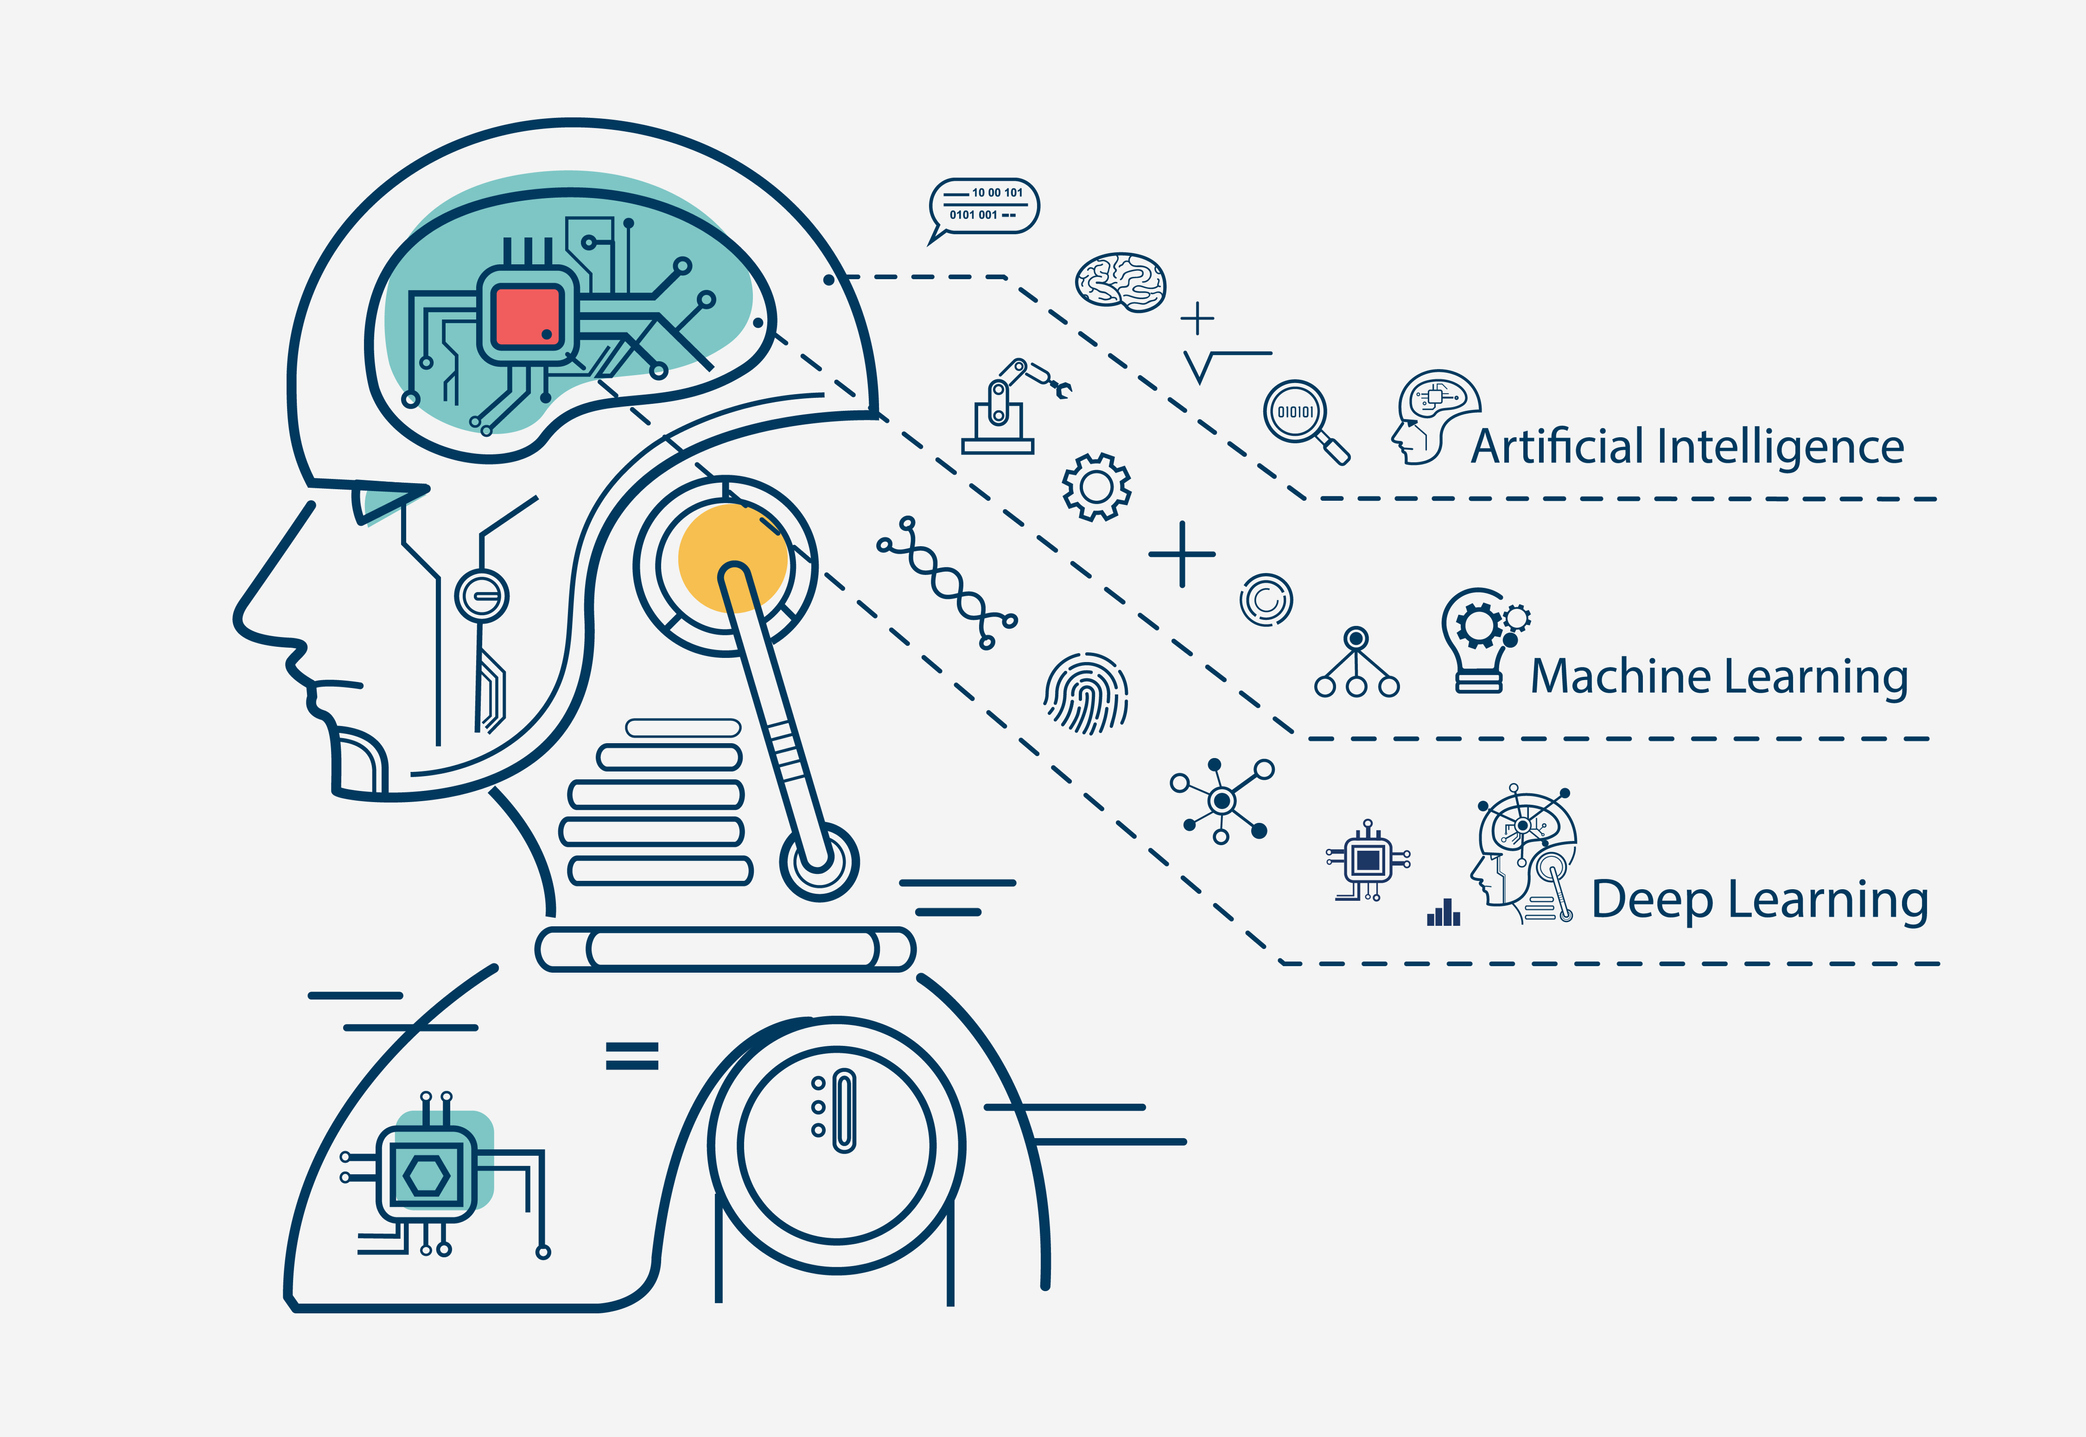
\includegraphics[width=1.0\textwidth]{./Images/deep_learning.jpg}
				\end{figure}
			\end{column}
		\end{columns}

	\end{frame}

	% --------- DETECTOR
	\section{The Detector}

	% ------ EXPERIMENT CONFIGURATION
	\begin{frame}
		\frametitle{The Detector}
		\framesubtitle{Experimental setup}

		\begin{columns}

			\begin{column}{0.55\framewidth}
				% --- DETECTOR FIGURE
				\vspace{-2.5em}
				\begin{center}
					\resizebox{!}{0.75\paperheight}{%
\begin{tikzpicture}

    % LOWER CHAMBER
    \foreach \i in {0,...,15}{
        \filldraw[color=black, fill=black!10, thick] (2*\i/3,     0*0.2) rectangle + (2*1/3, 0.2);
        \filldraw[color=black, fill=black!10, thick] (2*\i/3+1/3, 1*0.2) rectangle + (2*1/3, 0.2);
        \filldraw[color=black, fill=black!10, thick] (2*\i/3,     2*0.2) rectangle + (2*1/3, 0.2);
        \filldraw[color=black, fill=black!10, thick] (2*\i/3+1/3, 3*0.2) rectangle + (2*1/3, 0.2);
    }

    \filldraw[color=black, fill=black!10, thick] (0,      1*0.2) rectangle + (1/3, 0.2);
    \filldraw[color=black, fill=black!10, thick] (0,      3*0.2) rectangle + (1/3, 0.2);
    \filldraw[color=black, fill=black!10, thick] (2*16/3, 0*0.2) rectangle + (1/3, 0.2);
    \filldraw[color=black, fill=black!10, thick] (2*16/3, 2*0.2) rectangle + (1/3, 0.2);

    % LOWER SCINTILLATOR
    \filldraw[color=blue, fill=blue!10, thick] (17/3 - 2.5, 2.6) node[below left] {scintillator} rectangle + (5, 0.2);

    % ROTATED CHAMBER
    \foreach \i in {0,...,3}{
        \filldraw[color=black, fill=black!10, thick, opacity=0.7] (0, \i*0.2 + 2.9) rectangle + (2*1/3*16 + 1/3, 0.2);
    }

    % MIDDLE CHAMBER
    \foreach \i in {0,...,15}{
        \filldraw[color=black, fill=black!10, thick] (2*\i/3,     0*0.2 + 4.1) rectangle + (2*1/3, 0.2);
        \filldraw[color=black, fill=black!10, thick] (2*\i/3+1/3, 1*0.2 + 4.1) rectangle + (2*1/3, 0.2);
        \filldraw[color=black, fill=black!10, thick] (2*\i/3,     2*0.2 + 4.1) rectangle + (2*1/3, 0.2);
        \filldraw[color=black, fill=black!10, thick] (2*\i/3+1/3, 3*0.2 + 4.1) rectangle + (2*1/3, 0.2);
    }

    \filldraw[color=black, fill=black!10, thick] (0,      1*0.2 + 4.1) rectangle + (1/3, 0.2);
    \filldraw[color=black, fill=black!10, thick] (0,      3*0.2 + 4.1) rectangle + (1/3, 0.2);
    \filldraw[color=black, fill=black!10, thick] (2*16/3, 0*0.2 + 4.1) rectangle + (1/3, 0.2);
    \filldraw[color=black, fill=black!10, thick] (2*16/3, 2*0.2 + 4.1) rectangle + (1/3, 0.2);

    % UPPER SCINTILLATOR
    \filldraw[color=blue, fill=blue!10, thick] (17/3 - 2.5, 5) rectangle + (5, 0.2);

    % UPPER CHAMBER
    \foreach \i in {0,...,15}{
        \filldraw[color=black, fill=black!10, thick] (2*\i/3,     0*0.2 + 7) rectangle + (2*1/3, 0.2);
        \filldraw[color=black, fill=black!10, thick] (2*\i/3+1/3, 1*0.2 + 7) rectangle + (2*1/3, 0.2);
        \filldraw[color=black, fill=black!10, thick] (2*\i/3,     2*0.2 + 7) rectangle + (2*1/3, 0.2);
        \filldraw[color=black, fill=black!10, thick] (2*\i/3+1/3, 3*0.2 + 7) rectangle + (2*1/3, 0.2);
    }

    \filldraw[color=black, fill=black!10, thick] (0,      1*0.2 + 7) rectangle + (1/3, 0.2);
    \filldraw[color=black, fill=black!10, thick] (0,      3*0.2 + 7) rectangle + (1/3, 0.2);
    \filldraw[color=black, fill=black!10, thick] (2*16/3, 0*0.2 + 7) rectangle + (1/3, 0.2);
    \filldraw[color=black, fill=black!10, thick] (2*16/3, 2*0.2 + 7) rectangle + (1/3, 0.2);

    % ACTIVATED CELLS
    \filldraw[color=black, fill=red!40, thick] (2*7/3,      0*0.2) rectangle + (2/3, 0.2);
    \filldraw[color=black, fill=red!40, thick] (2*7/3+1/3,  1*0.2) rectangle + (2/3, 0.2);
    \filldraw[color=black, fill=red!40, thick] (2*7/3,      2*0.2) rectangle + (2/3, 0.2);
    \filldraw[color=black, fill=red!40, thick] (2*7/3+1/3,  3*0.2) rectangle + (2/3, 0.2);

    \filldraw[color=black, fill=red!40, thick] (2*8/3,      0*0.2 + 4.1) rectangle + (2/3, 0.2);
    \filldraw[color=black, fill=red!40, thick] (2*8/3+1/3,  1*0.2 + 4.1) rectangle + (2/3, 0.2);
    \filldraw[color=black, fill=red!40, thick] (2*8/3,      2*0.2 + 4.1) rectangle + (2/3, 0.2);
    \filldraw[color=black, fill=red!40, thick] (2*8/3+1/3,  3*0.2 + 4.1) rectangle + (2/3, 0.2);

    \filldraw[color=black, fill=red!40, thick] (2*9/3,      0*0.2 + 7) rectangle + (2/3, 0.2);
    \filldraw[color=black, fill=red!40, thick] (2*8/3+1/3,  1*0.2 + 7) rectangle + (2/3, 0.2);
    \filldraw[color=black, fill=red!40, thick] (2*9/3,      2*0.2 + 7) rectangle + (2/3, 0.2);
    \filldraw[color=black, fill=red!40, thick] (2*8/3+1/3,  3*0.2 + 7) rectangle + (2/3, 0.2);

    % MUON TRACK
    \draw[color=red, very thick] (17/3-0.6, -0.5) -- (17/3+0.7, 8.3) node[right] {muon track};


    \node(cell) at (17/3-2, -3) {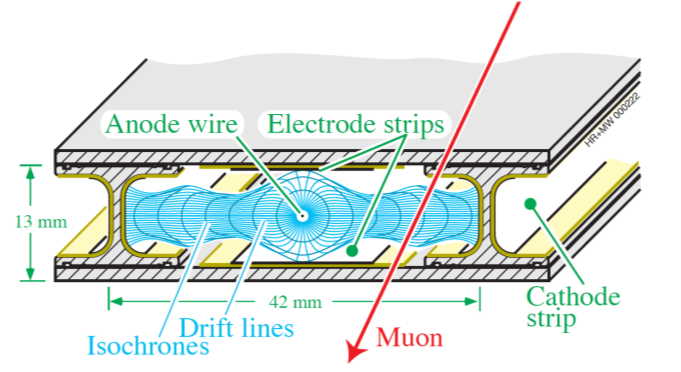
\includegraphics[width=1.4\textwidth]{./Images/cell.png}}; 
    
    \draw[bend left,<-, very thick, shorten <=2pt, shorten >=2pt] (cell) to node[midway,right] {drift tube} (1/3,0.1) ;

    \node(eq)[below right = -3cm and 0.5cm of cell, scale=2, rectangle, fill=yellow!50] {$x=\pm \,
    v_{\text{drift}}\,\underbrace{(t-t_0)}_{\text{\alert{drift time}}}$};
         
\end{tikzpicture}
}
				\end{center}

				% \vfill

			\end{column}

			\begin{column}{0.45\framewidth}
				\vspace{-5.5em}
				% --- BULLETPOINTS
				\begin{itemize}
					\setlength{\itemsep}{1em}
					\item 4 muon chambers (\alert{\textit{superlayers}})
					\item 4 staggered layers of 16 \alert{\textit{drift tubes}} each
					\item \alert{\textit{trigger-less}} data acquisition system
					\item 2 \alert{\textit{scintillator}} tiles		
				\end{itemize}
				% \vfill
			\end{column}
			
		\end{columns}

		
		
	\end{frame}

	% --------- DRIFT TIME
	\section{DriftTime}
	\begin{frame}
		\frametitle{The Drift Time Distribution}
		\framesubtitle{Main features of the time box}
		% --- BULLETPOINTS
		\begin{alertblock}{}
			Collection of the times that the electrons take to reach the anodic wire in the center of the cell
		\end{alertblock}
		The external trigger 
		\begin{itemize}
			\item allows to discriminate \alert{\textit{muon hits}} from background noise
			\item provides a \alert{\textit{timing reference} $t_0$} for computing the drift time
		\end{itemize}

		\begin{columns}
			% LEFT COLUMN
			\begin{column}{0.5\textwidth}
				\begin{figure}
					\centering 
					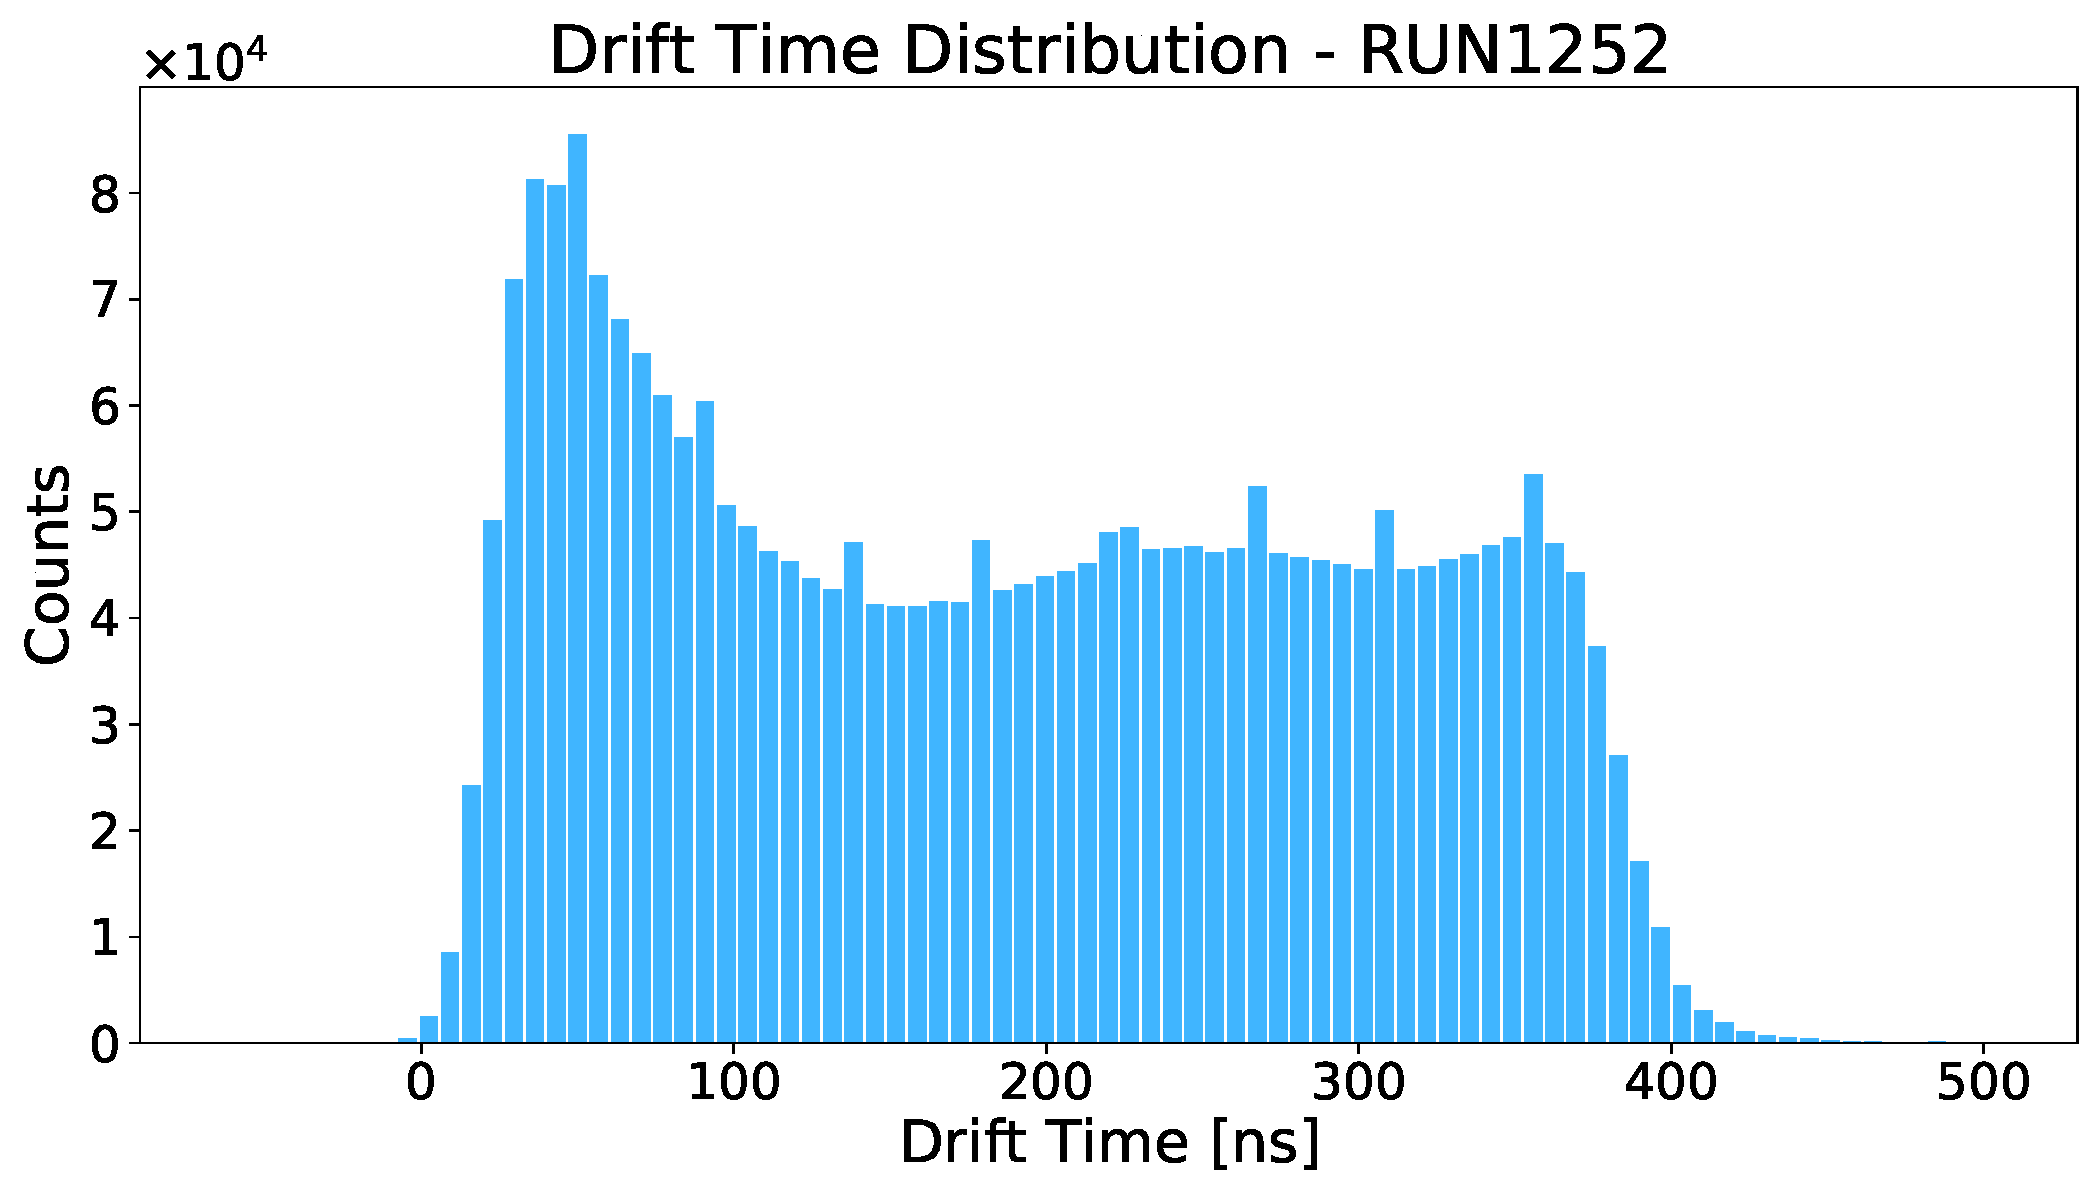
\includegraphics[width=1.0\textwidth]{../PLOTS/DRIFT_TIME/thesis/run1252_shifted.pdf}
				\end{figure}
			\end{column}
			% RIGHT COLUMN
			\begin{column}{0.5\textwidth}
				Time box shape:
				\begin{itemize}
					\item approximately \alert{\textit{uniform}}
					\item $\sim$\alert{$400\,\si{\nano\second}$} width
				\end{itemize}
			\end{column}
		\end{columns}
	\end{frame}

	% --------- THE DEEP LEARNING ALGORITHM
	\section{The Deep Learning Algorithm}
	\begin{frame}
		\frametitle{The Deep Learning Algorithm}
		\framesubtitle{A brief overview}
		% --- SUMMARY FIGURE
		\tikzset{circ/.style={circle, inner sep=0pt, minimum size=0.8cm, fill=blue!50, draw=black, text=white, align=center}}


\resizebox{\framewidth}{!}{%
\begin{tikzpicture}
 
    % MAIN RECTANGLE
    \node(main)[label={[label distance=1cm]above:\bfseries NEURAL NETWORK}] 
    {\tikz {\filldraw[thick,rounded corners=15pt,fill=orange!50] (-3,-2) rectangle (3,2);}};
        

    % INSIDE
    \node(first-circle)[circ, minimum size=1.4cm, thick] at (-0.5,1.1) {model \\ $w$};
    \node(second-circle)[circ, minimum size=1.4cm, thick] at (-0.5,-1.1) {model \\ $\hat{w}$};

    \draw[bend right,->, very thick, shorten <=2pt, shorten >=2pt]  (first-circle) to node [auto] 
    {\bfseries training $\mathbfcal{D}$ vs $\mathbfcal{R}$} (second-circle);

    \draw[thick] (-2.0,1.1) -- (first-circle);
    \node(point-1)[circ, minimum size=0.1cm, fill=black, label=left:{$\boldsymbol{x}$}] at (-2.0,1.1) {};

    \draw[thick] (first-circle) -- (1.0,1.1);
    \node(point-2)[circ, minimum size=0.1cm, fill=black, label=right:{$\boldsymbol{f(x;\,w)}$}] at (1.0,1.1) {};

    \draw[thick] (-2.0,-1.1) -- (second-circle);
    \node(point-3)[circ, minimum size=0.1cm, fill=black, label=left:{$\boldsymbol{x}$}] at (-2.0,-1.1) {};

    \draw[thick] (second-circle) -- (1.0,-1.1);
    \node(point-4)[circ, minimum size=0.1cm, fill=black, label=right:{$\boldsymbol{f(x;\,\hat{w})}$}] at (1.0,-1.1) {};


    % UPPER LEFT
    \node(ref)[above left = -1cm and 0cm of main, label={[label distance=-0.4cm]above:\bfseries reference sample $\mathbfcal{R}$}] 
    {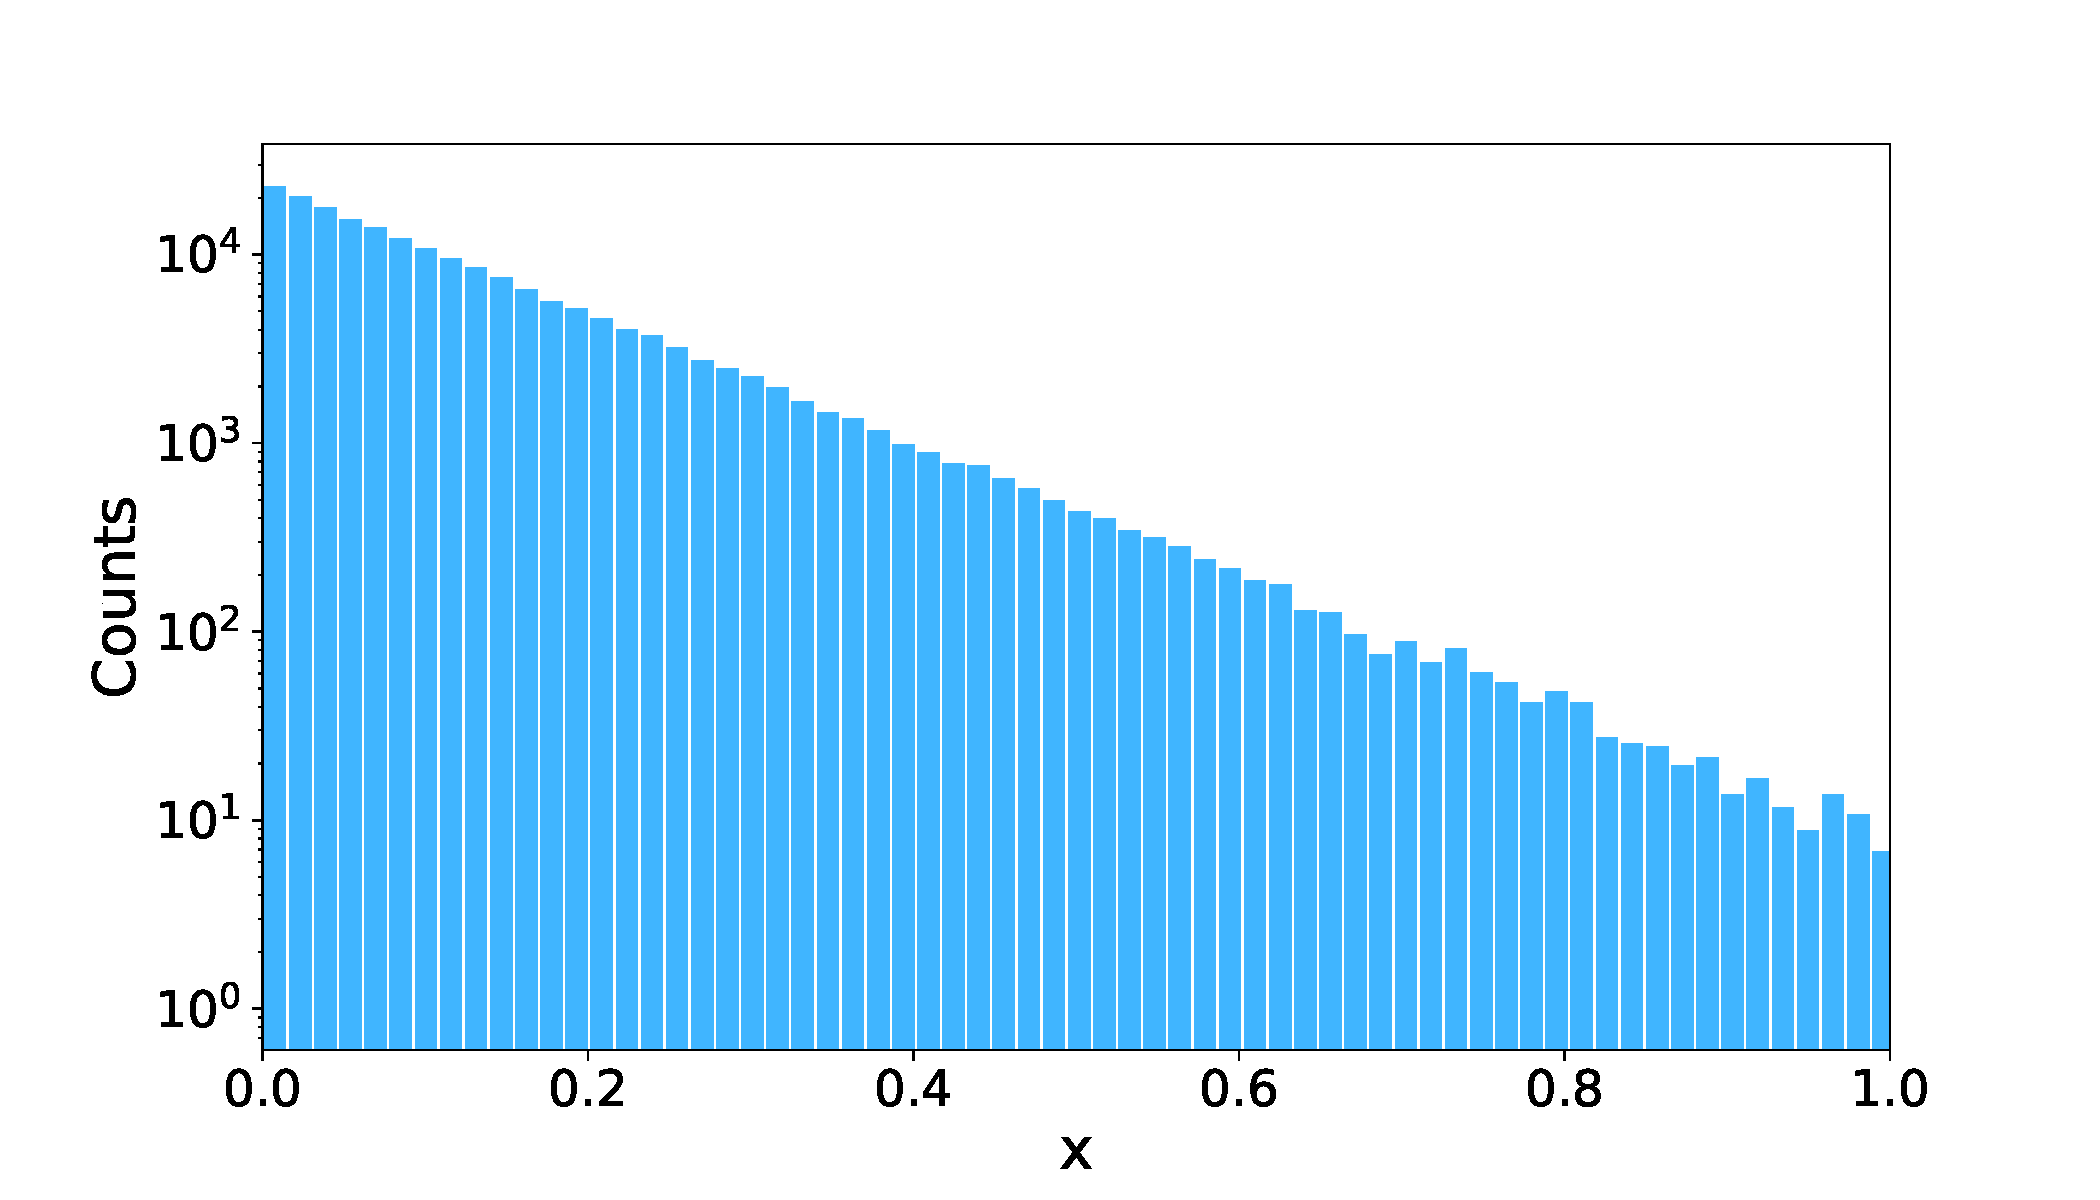
\includegraphics[width=.3\textwidth]{../PLOTS/DISTRIBUTIONS/ref.pdf}};
    \draw[bend left,->, very thick, shorten <=2pt, shorten >=2pt]  (ref) to node [auto] 
    {} (main);


    % LOWER LEFT
    \node(exp)[below left = -1cm and 0cm of main, label={[label distance=-0.4cm]above:\bfseries  data sample $\mathbfcal{D}$}]  
    {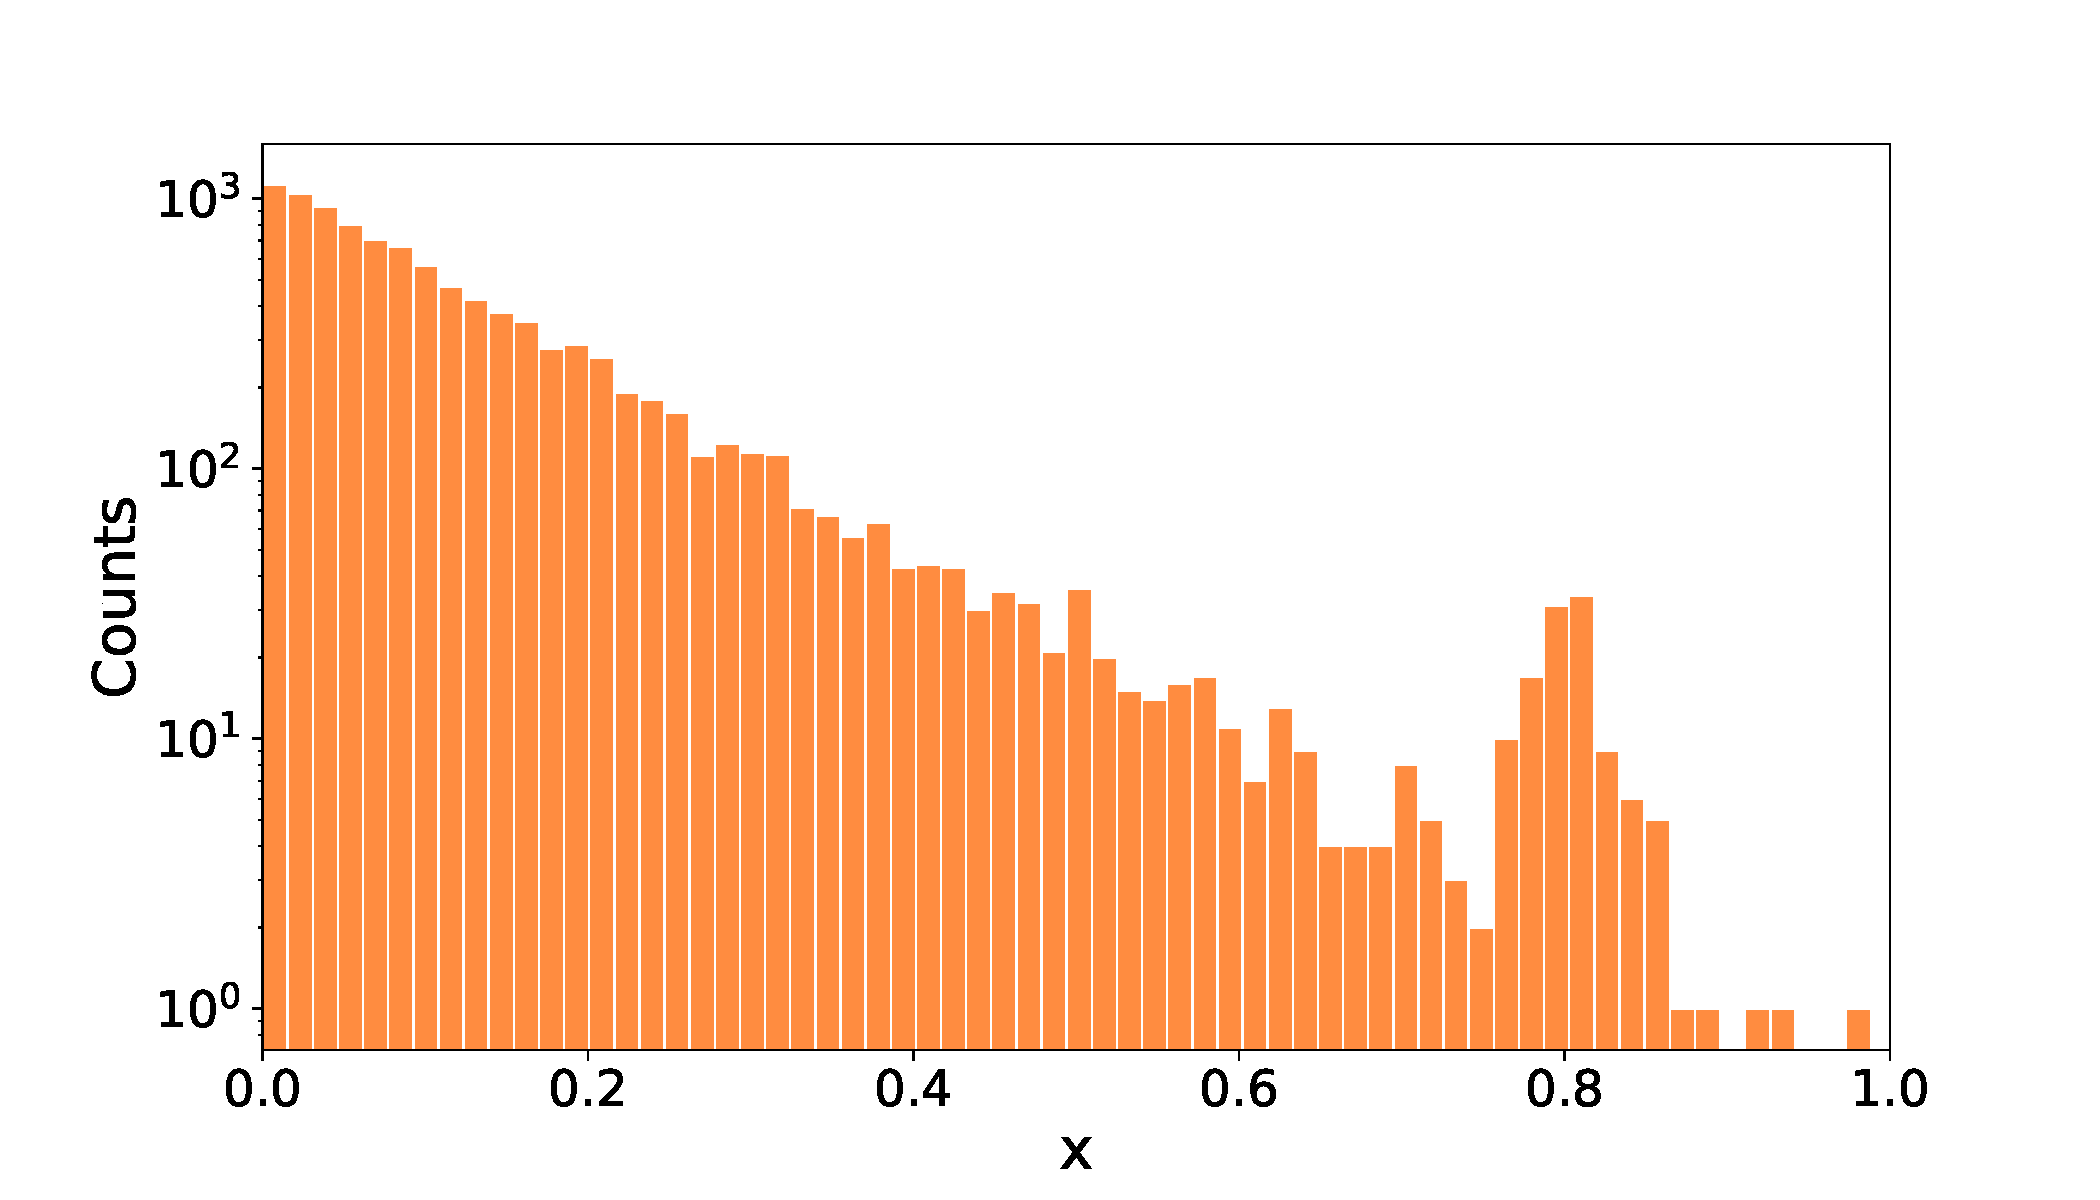
\includegraphics[width=.3\textwidth]{../PLOTS/DISTRIBUTIONS/exp.pdf}};
    \draw[bend right,->, very thick, shorten <=2pt, shorten >=2pt]  (exp) to node [auto] 
    {} (main);

    % UPPER RIGHT
    \node(log)[above right = -1cm and 0cm of main, label={[align=center, label distance=-0.4cm]above:\bfseries  log-ratio distribution \\ 
    $f(x;\,\hat{w})\approx \log\left[\frac{n(x\,|\,\mathbfcal{T})}{n(x\,|\,\mathbfcal{R})}\right]$}] 
    {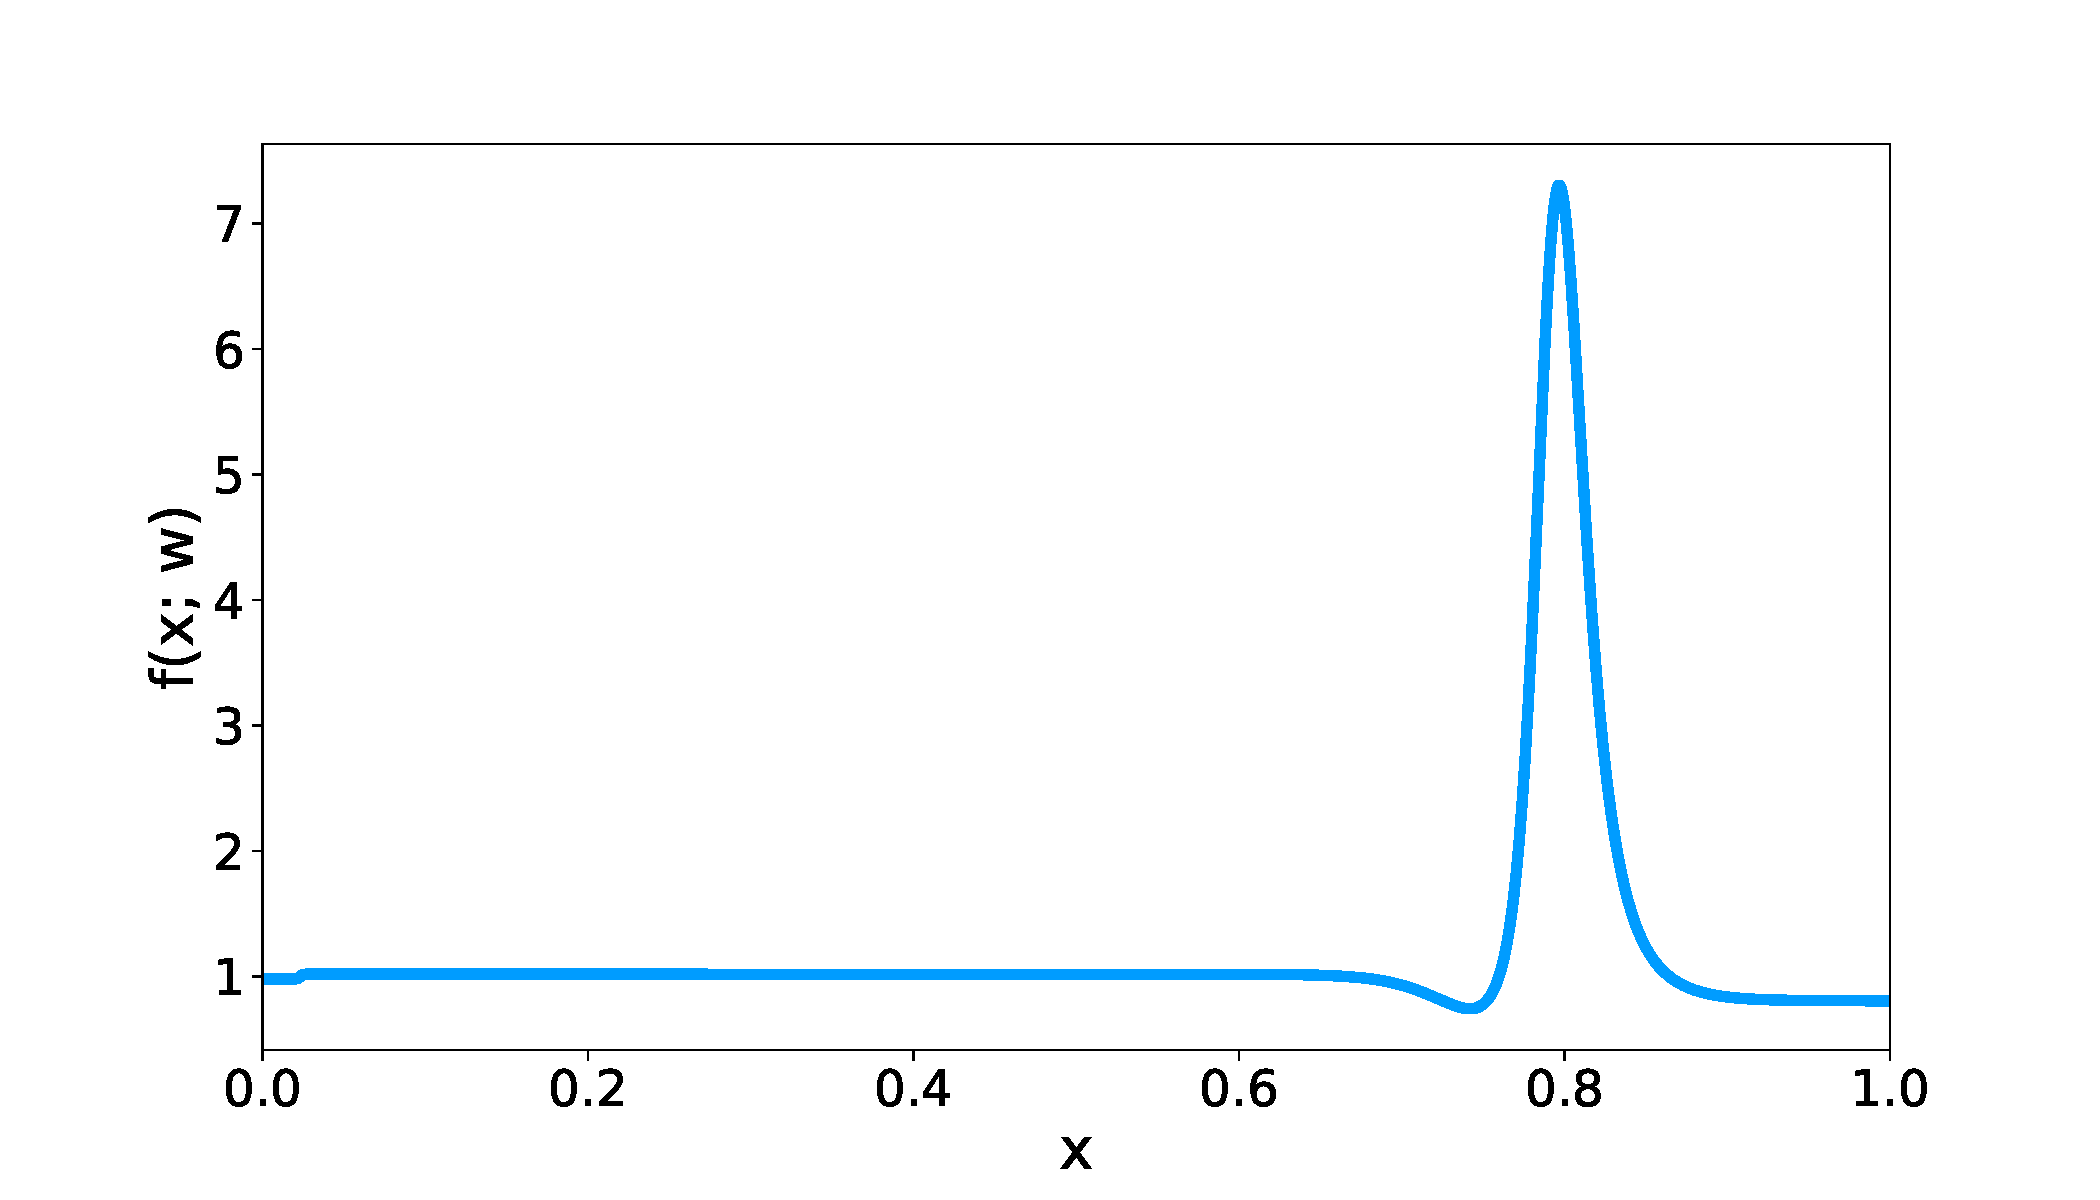
\includegraphics[width=.3\textwidth]{../PLOTS/DISTRIBUTIONS/log_ratio_47.pdf}};
    \draw[bend left,->, very thick, shorten <=2pt, shorten >=2pt]  (main) to node [auto] 
    {} (log);


    % LOWER RIGHT
    \node(t)[below right = -1cm and 0cm of main, label={[align=center, label distance=-0.4cm]above:\bfseries $\boldsymbol{t}$ distribution \\
    $t(\mathbfcal{D})=-2\,\min_w L[f]$}]  
    {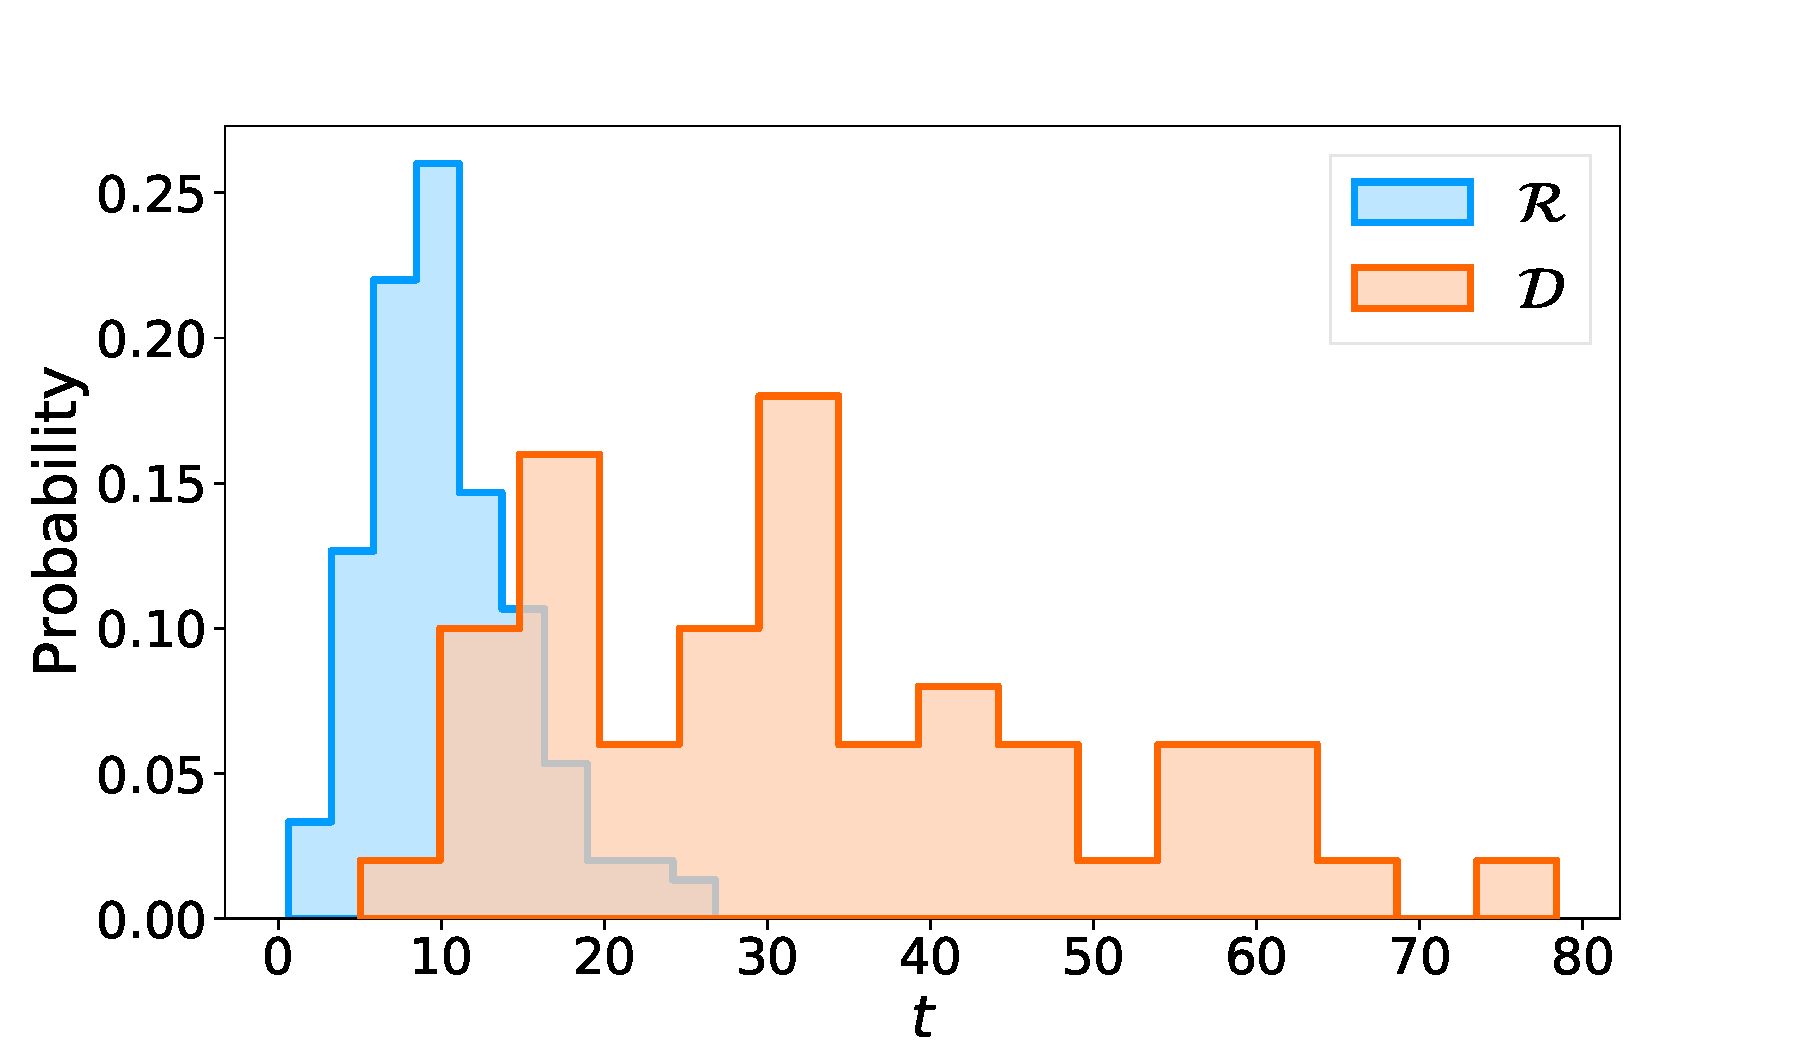
\includegraphics[width=.3\textwidth]{../PLOTS/DISTRIBUTIONS/summary_distribution.pdf}};
    \draw[bend right,->, very thick, shorten <=2pt, shorten >=2pt]  (main) to node [auto] 
    {} (t);

    % INPUT
    \node(in)[above = 1.5cm of ref]{\bfseries INPUT};

    % OUTPUT
    \node(out)[above = 1.5cm of log]{\bfseries OUTPUT};

\end{tikzpicture}}
	\end{frame}

	% --------- PROCEDURE

	% ------ TUNING
	\begin{frame}
		\frametitle{Tuning the Neural Network}
		\framesubtitle{Training the network on the reference dataset}

		\begin{columns}
			% LEFT COLUMN
			\begin{column}{0.5\textwidth}
				\begin{alertblock}{Reference sample $\mathbfcal{R}$}
					\begin{figure}
						\centering 
						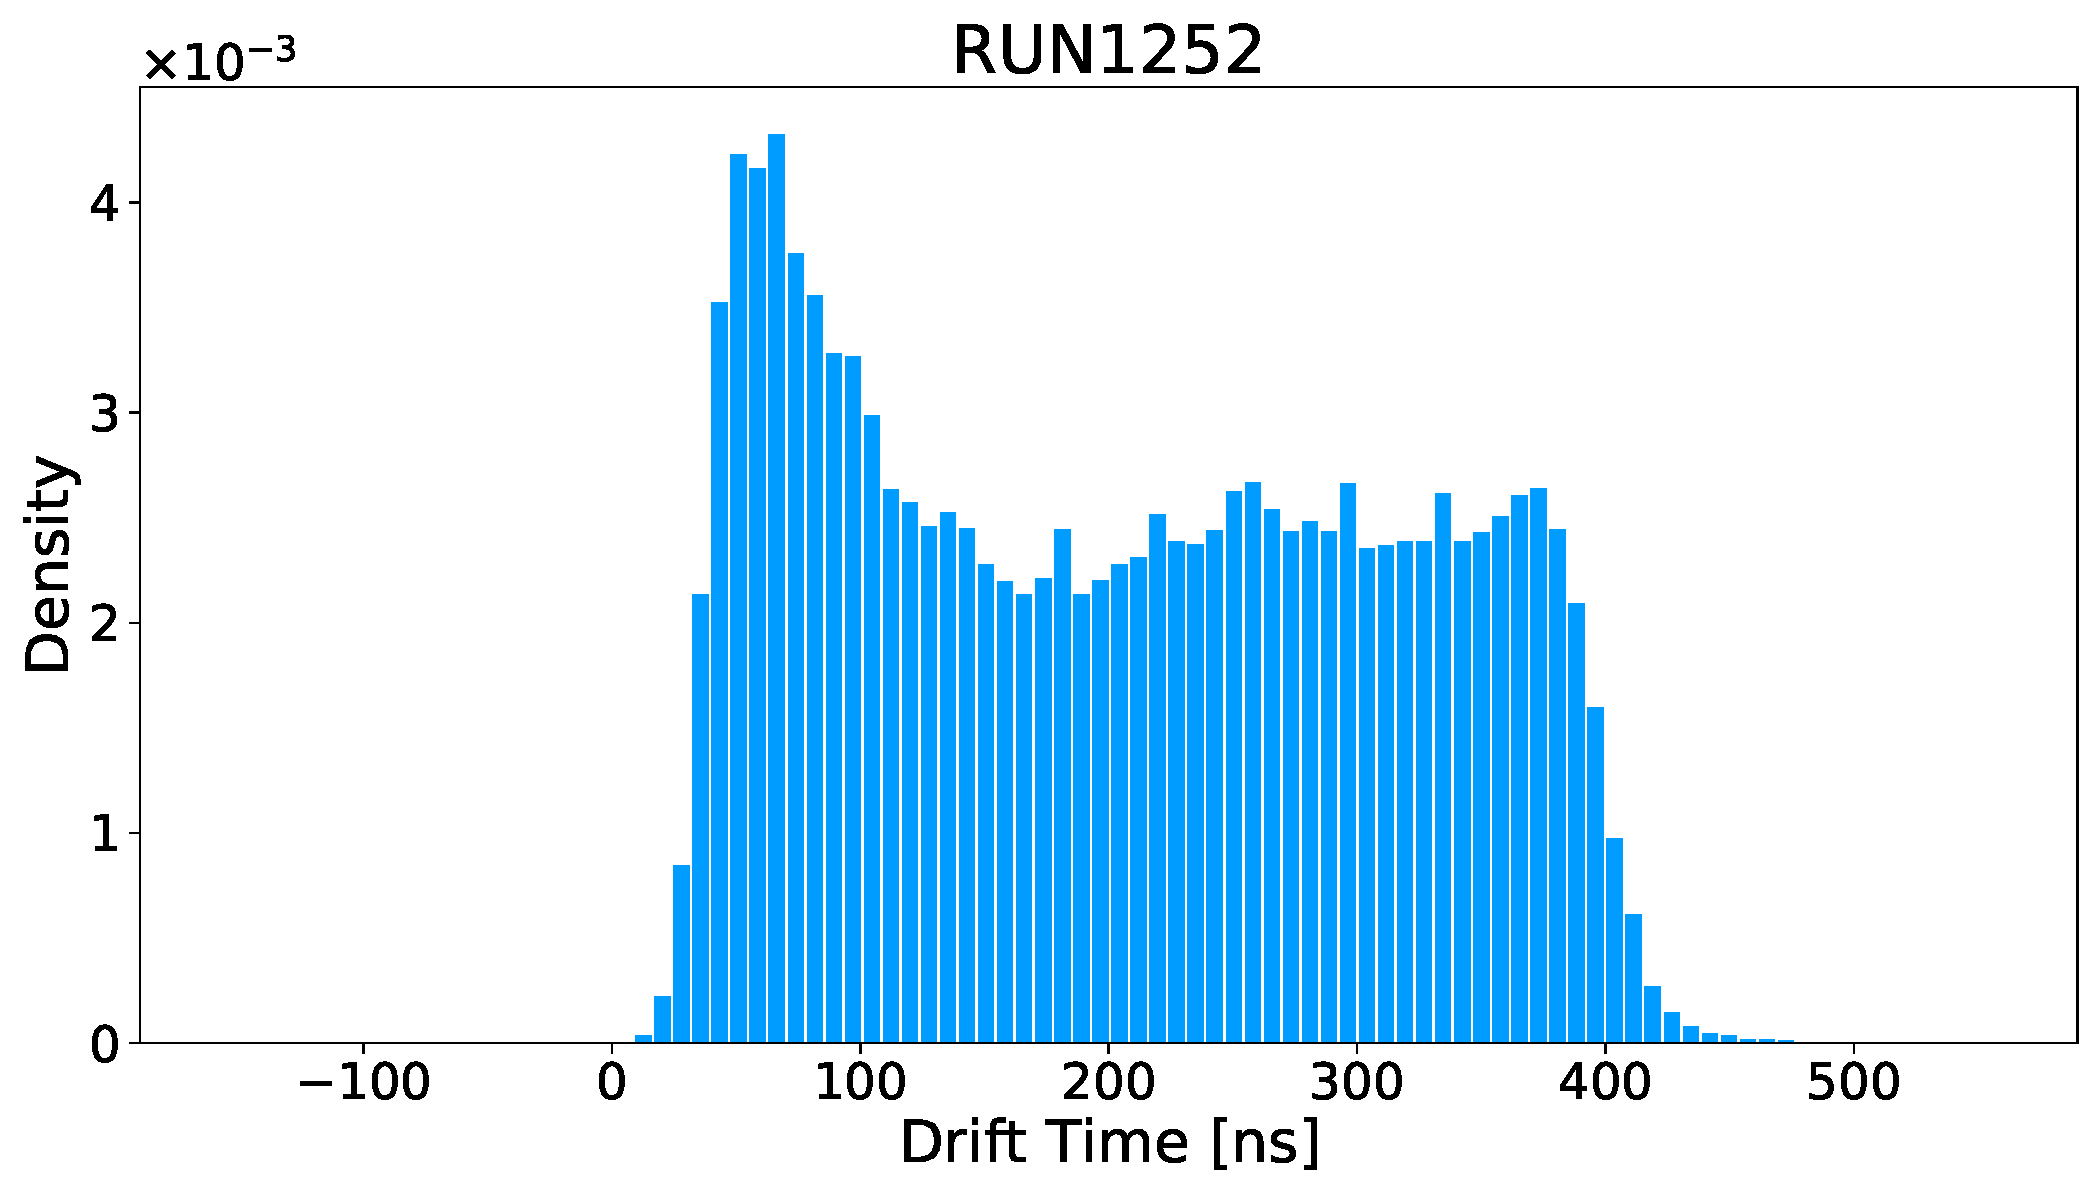
\includegraphics[width=1.0\textwidth]{./Images/reference.pdf}
					\end{figure}
					$\mathcal{N}_{\mathbfcal{R}}=200000$
				\end{alertblock}
			\end{column}
			% RIGHT COLUMN
			\begin{column}{0.5\textwidth}
				\begin{alertblock}{Data sample $\mathbfcal{D}$}
					\begin{figure}
						\centering 
						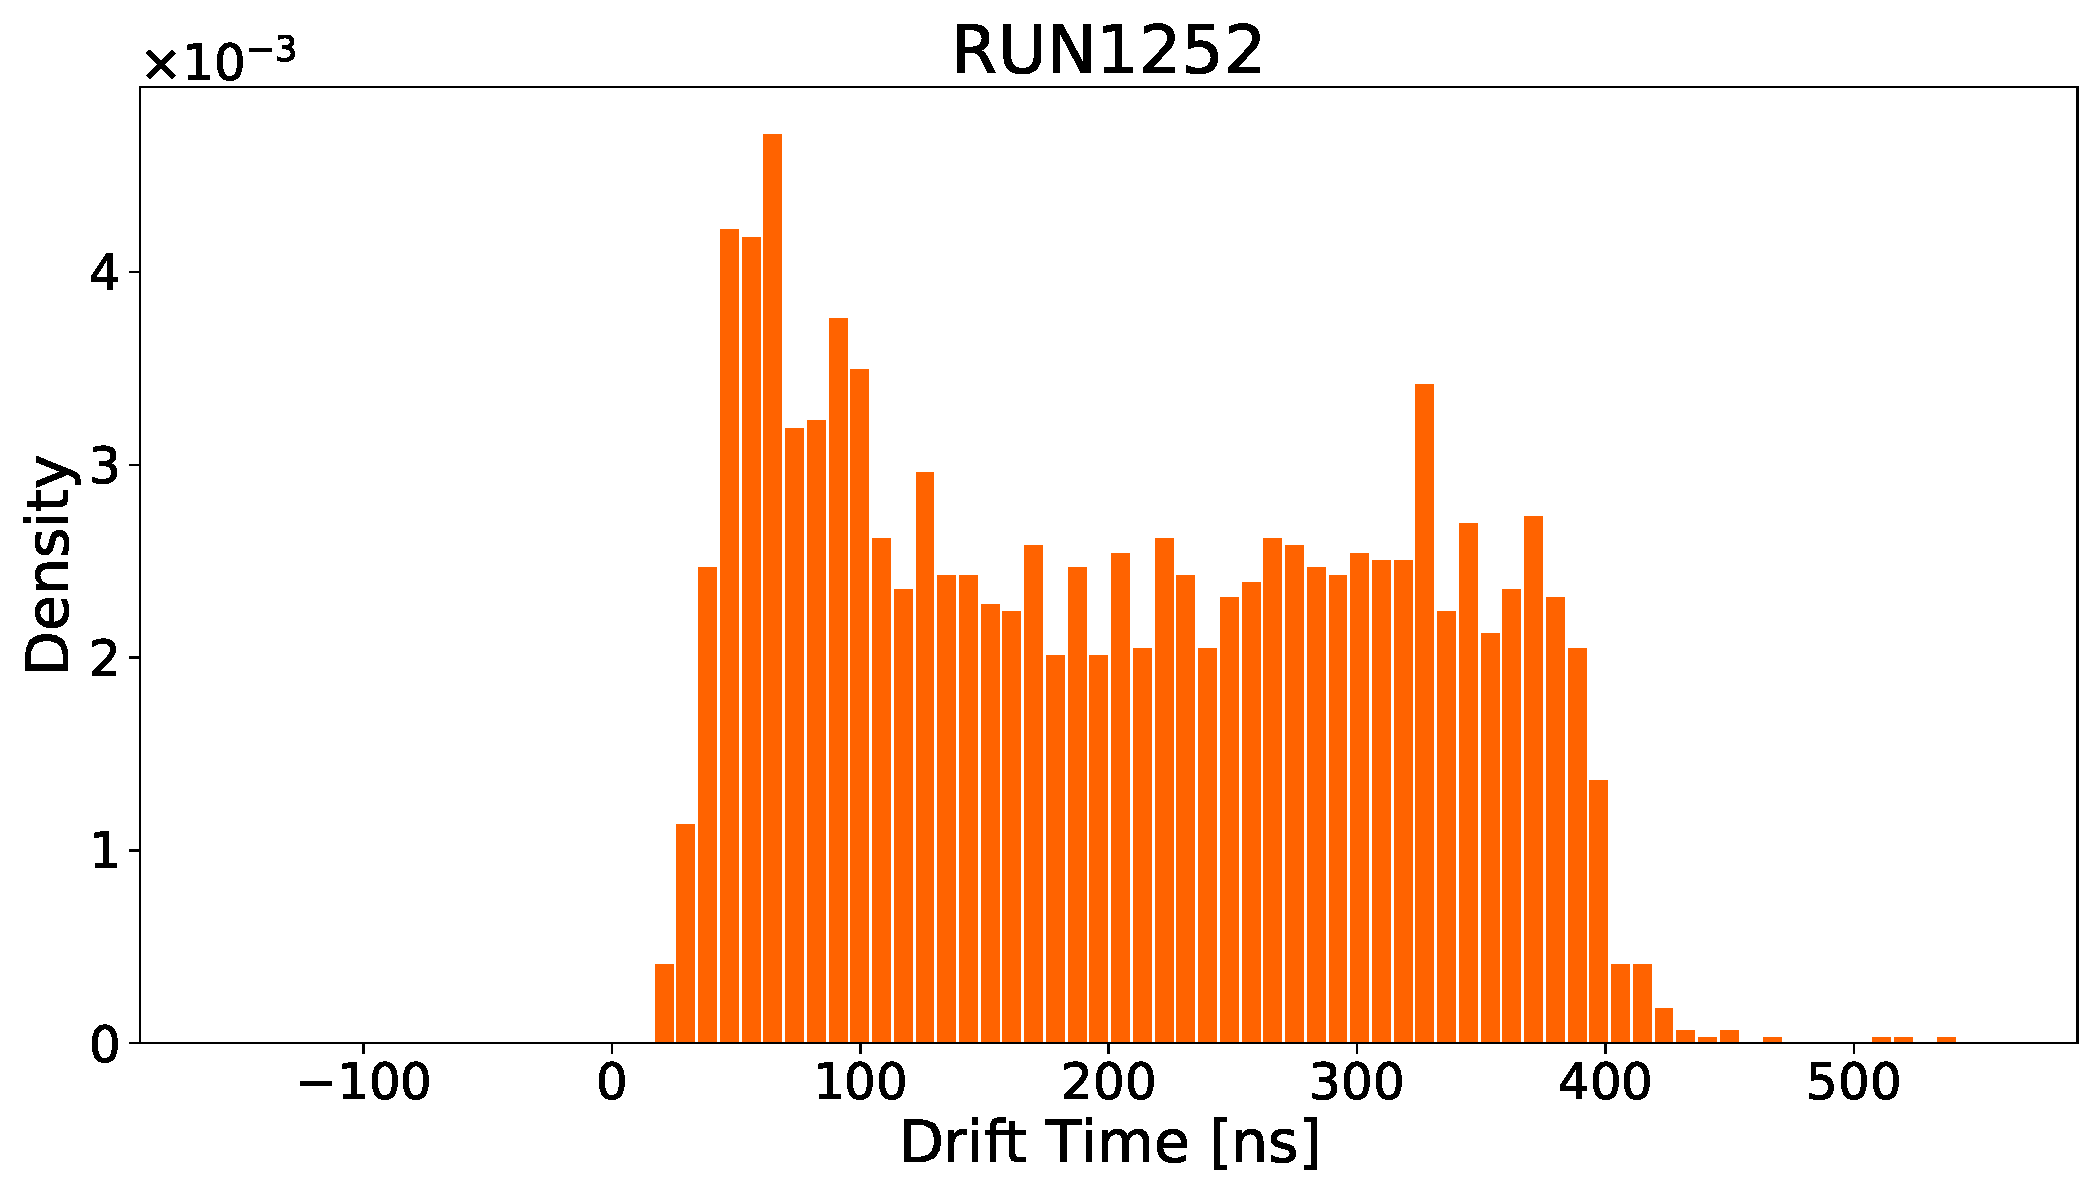
\includegraphics[width=1.0\textwidth]{./Images/sampled_ref.pdf}
					\end{figure}
					$\mathcal{N}_{\mathbfcal{D}}=3000$ sampled from $\mathbfcal{R}$
				\end{alertblock}
			\end{column}
		\end{columns}
	\end{frame}	

	

	% ------ TUNING
	\begin{frame}
		\frametitle{Tuning the Neural Network}
		\framesubtitle{Optimal weight clipping}

		\begin{columns}
			% LEFT COLUMN
			\begin{column}{0.5\textwidth}
				\begin{alertblock}{Test statistic distribution}
					\begin{figure}
						\centering 
						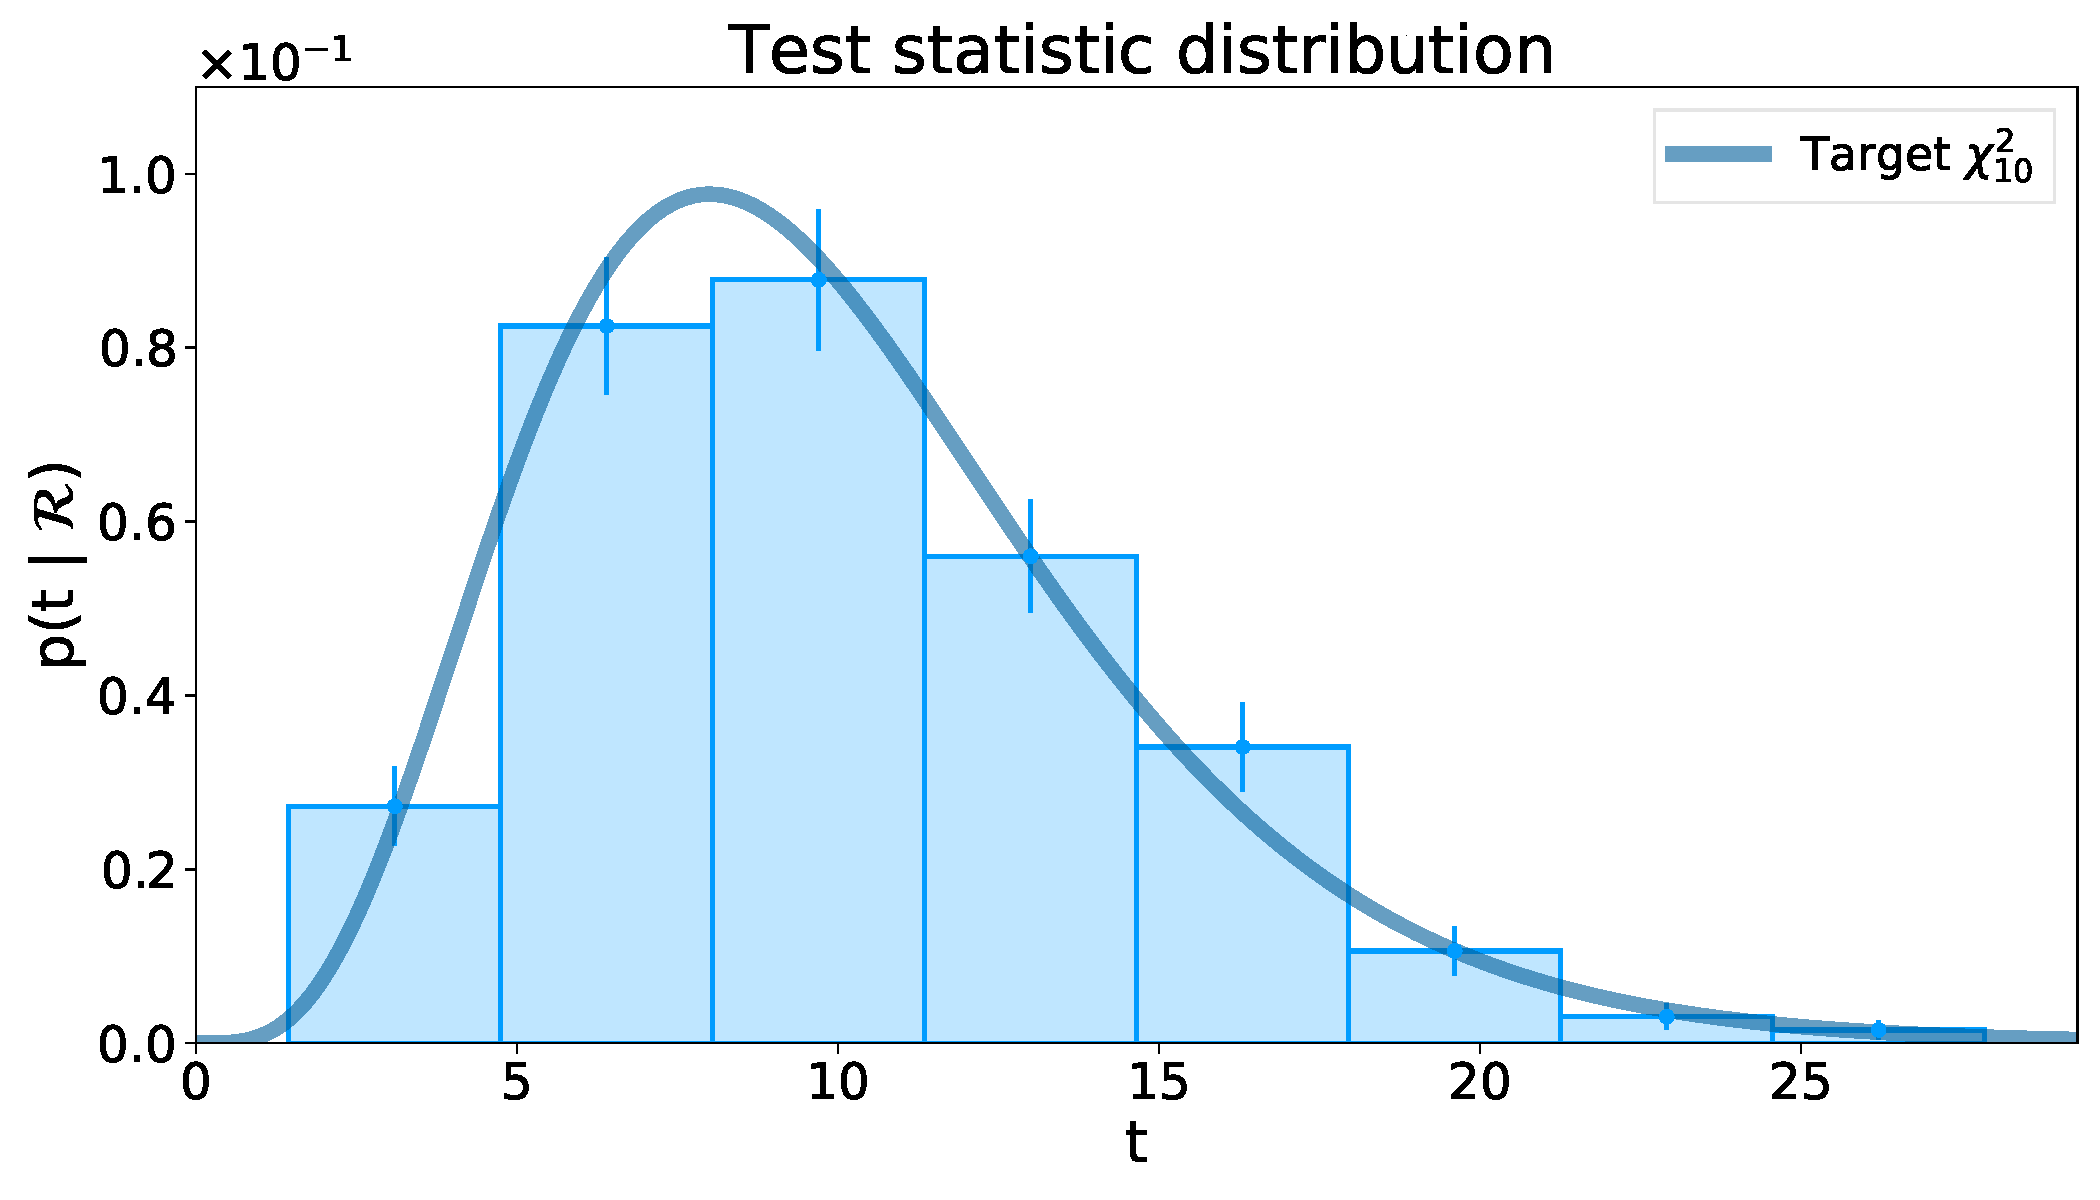
\includegraphics[width=1.0\textwidth]{../PLOTS/DRIFT_TIME/thesis/t_reference.pdf}
					\end{figure}
				\end{alertblock}	
			\end{column}
			% RIGHT COLUMN
			\begin{column}{0.5\textwidth}
				\begin{alertblock}{Quantiles evolution}
					\begin{figure}
						\centering 
						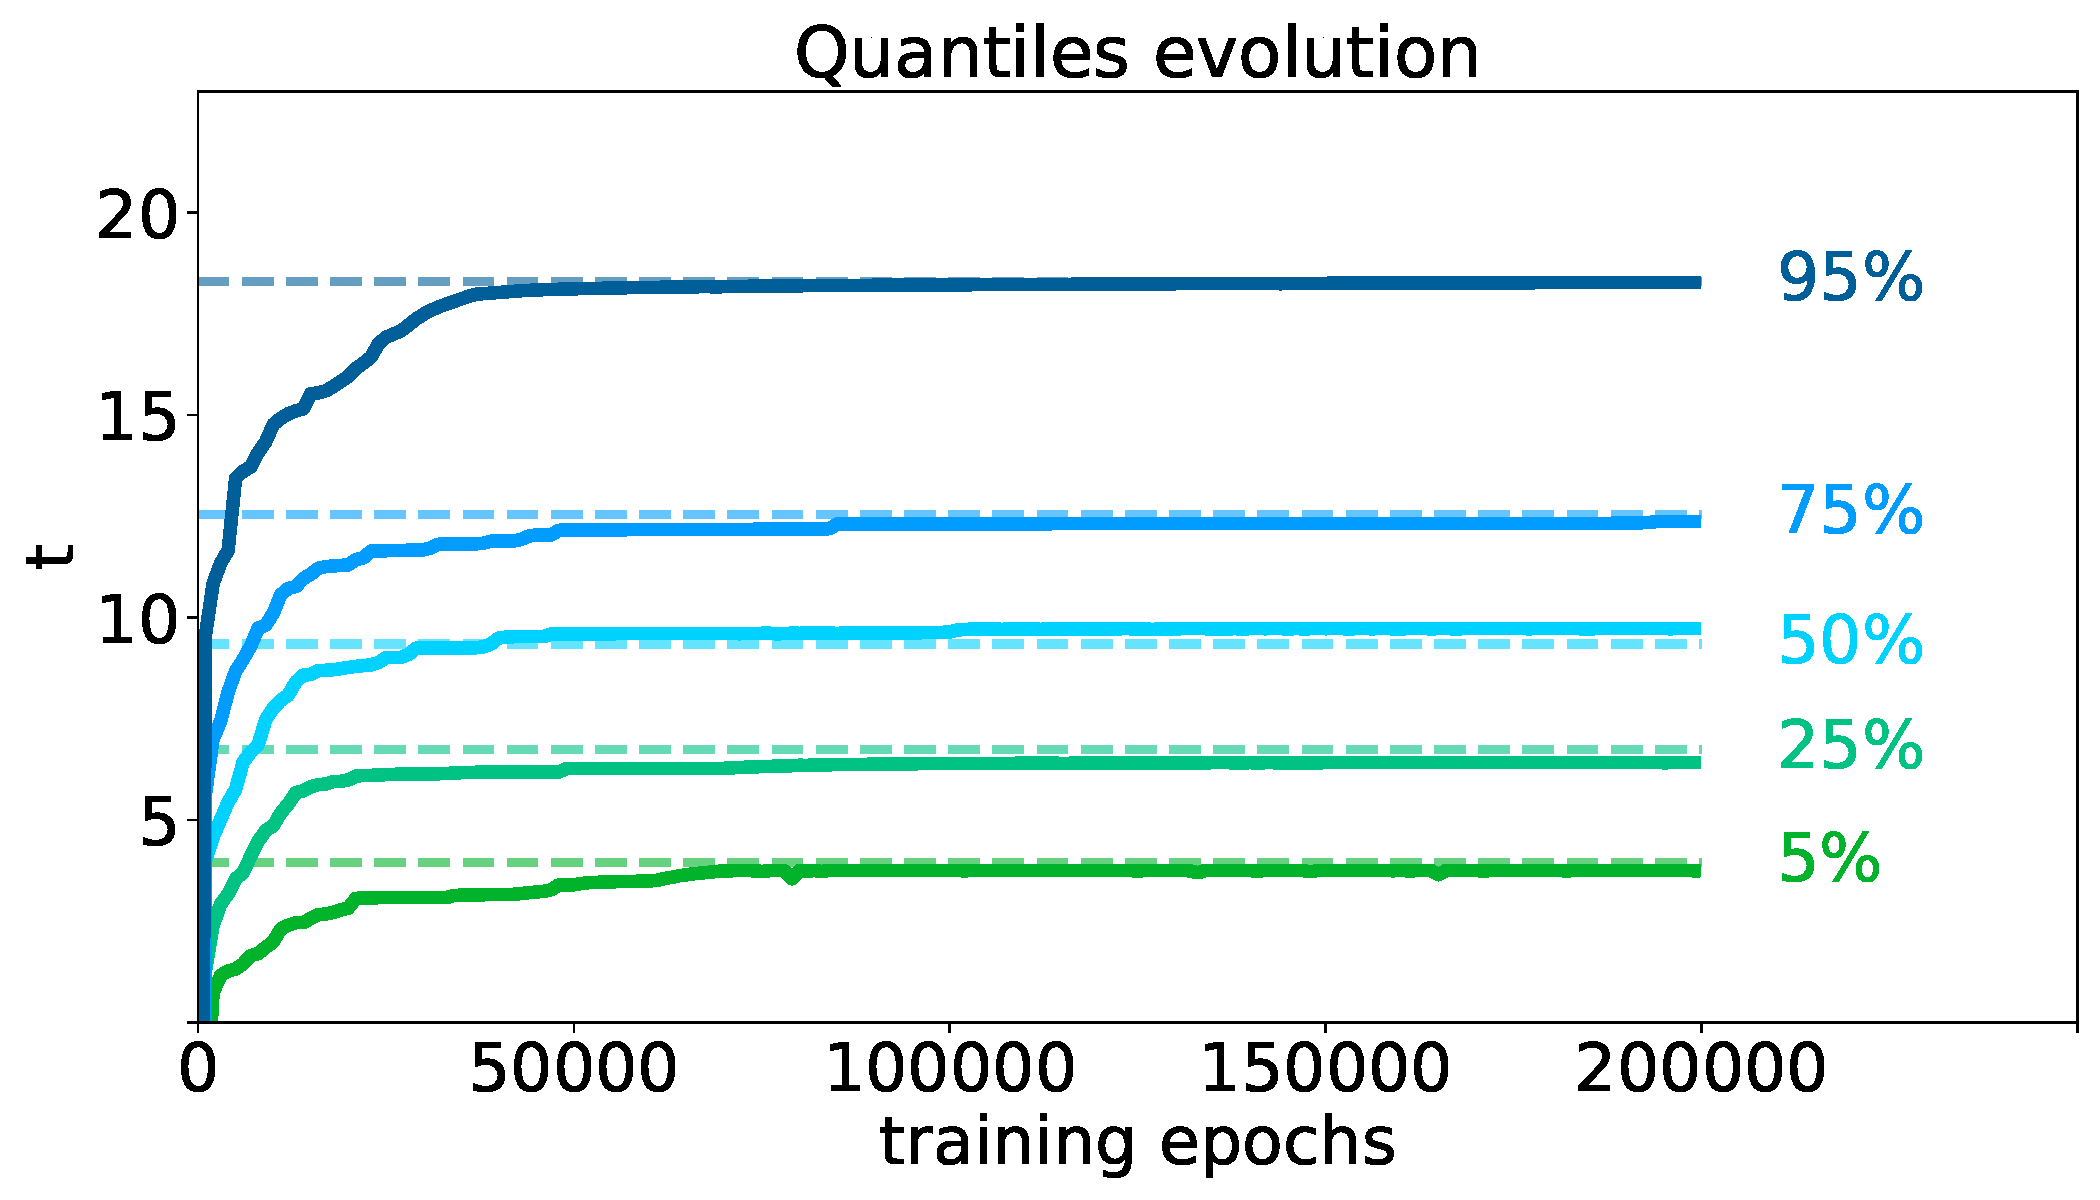
\includegraphics[width=1.0\textwidth]{../PLOTS/DRIFT_TIME/thesis/a_reference_quantiles.pdf}
					\end{figure}
				\end{alertblock}
			\end{column}
		\end{columns}

		\vfill
		400 samples of $\mathcal{N}_{\mathbfcal{D}}=3000$ each 

	\end{frame}


	% ------ DISTRIBUTIONS
	\begin{frame}
		\frametitle{Testing the algorithm performance}
		\framesubtitle{Drift time distributions}

		\vspace{-1.5em}

		\only{
			\begin{columns}%[onlytextwidth]

			% LEFT COLUMN
			\begin{column}{0.5\textwidth}

					\begin{figure}
						\centering 
						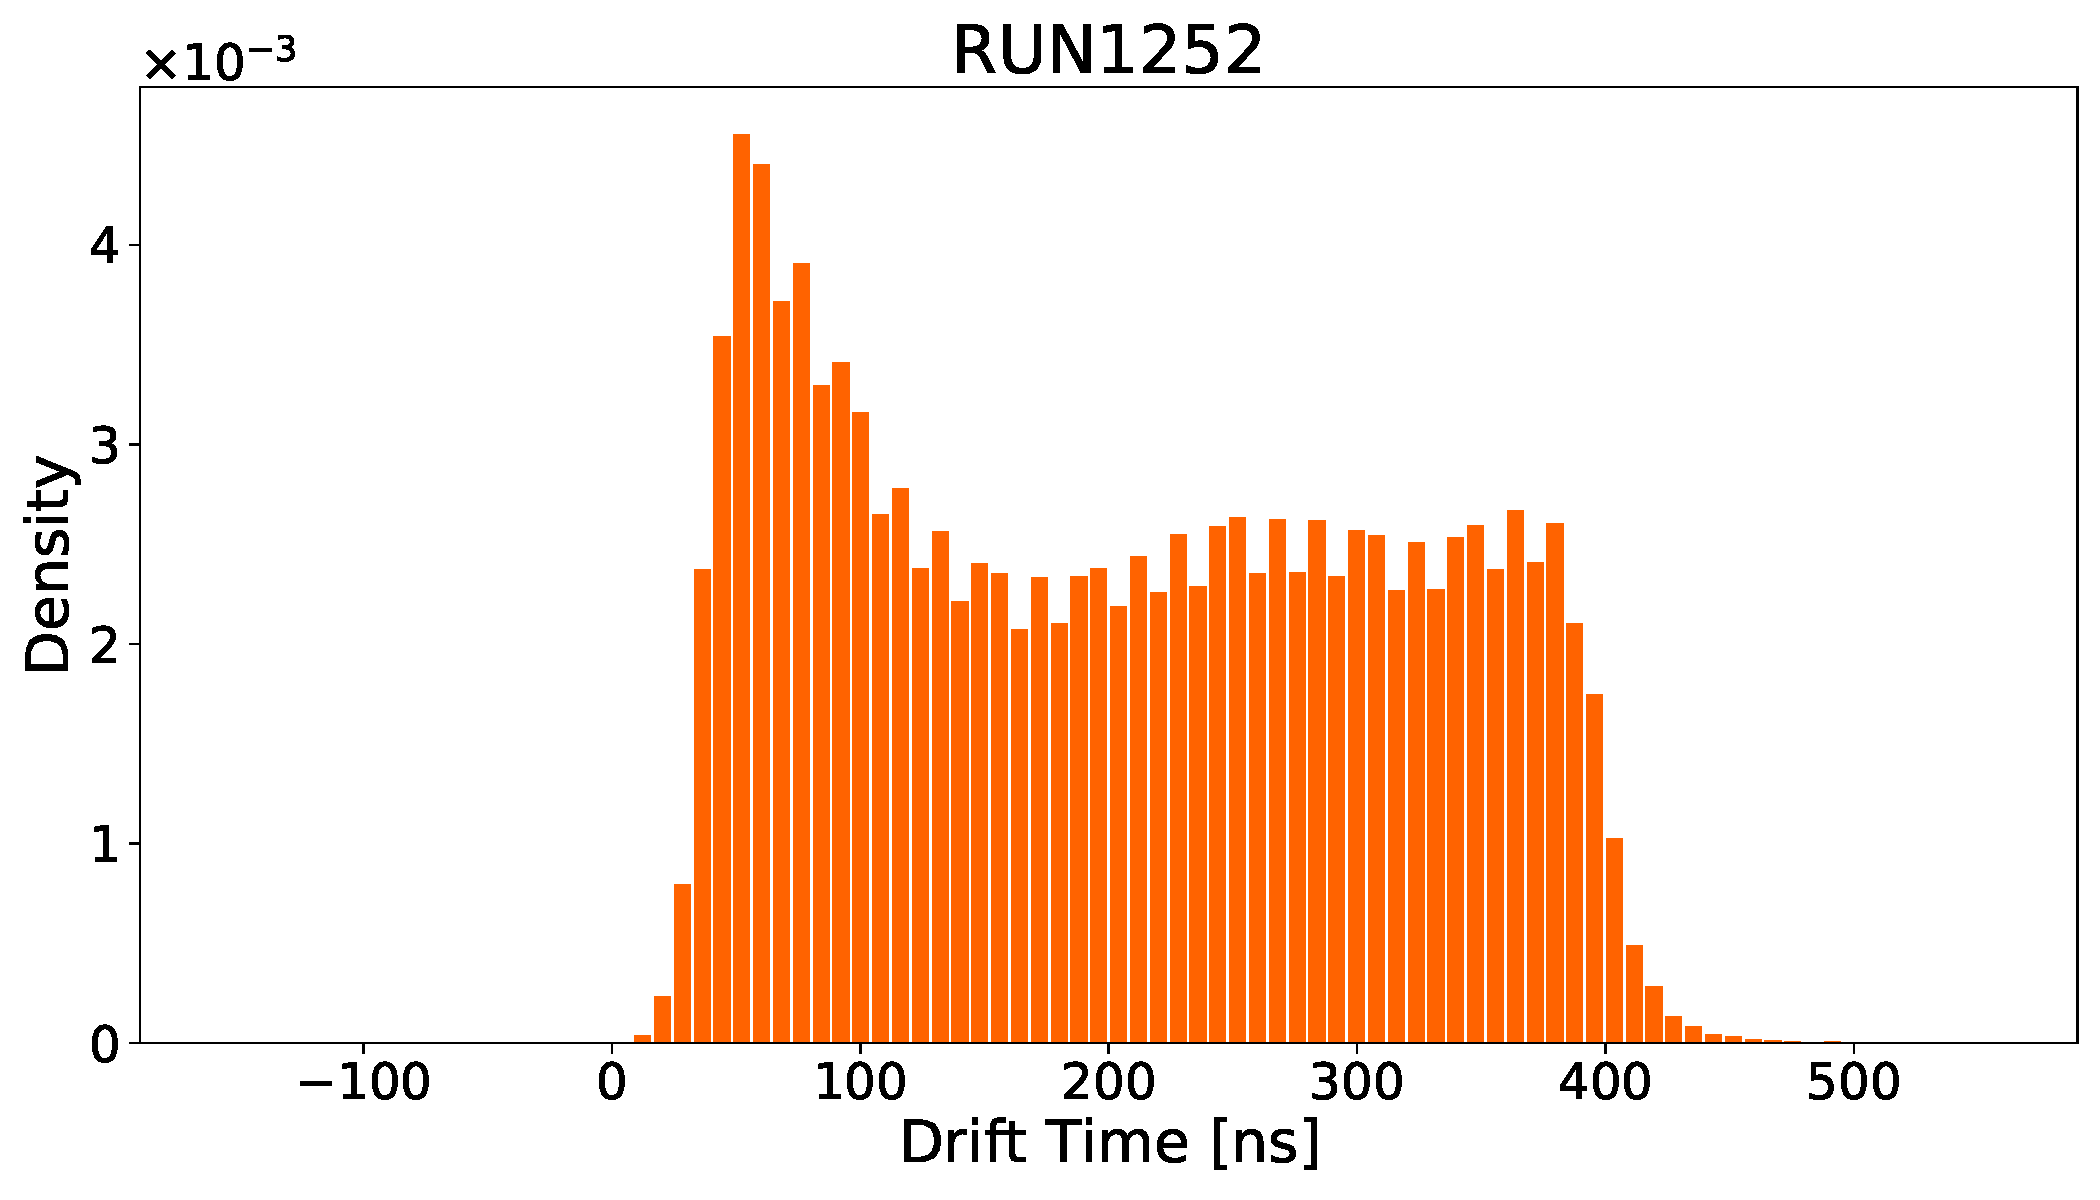
\includegraphics[width=1.0\textwidth]	{./Images/reference_orange.pdf}
						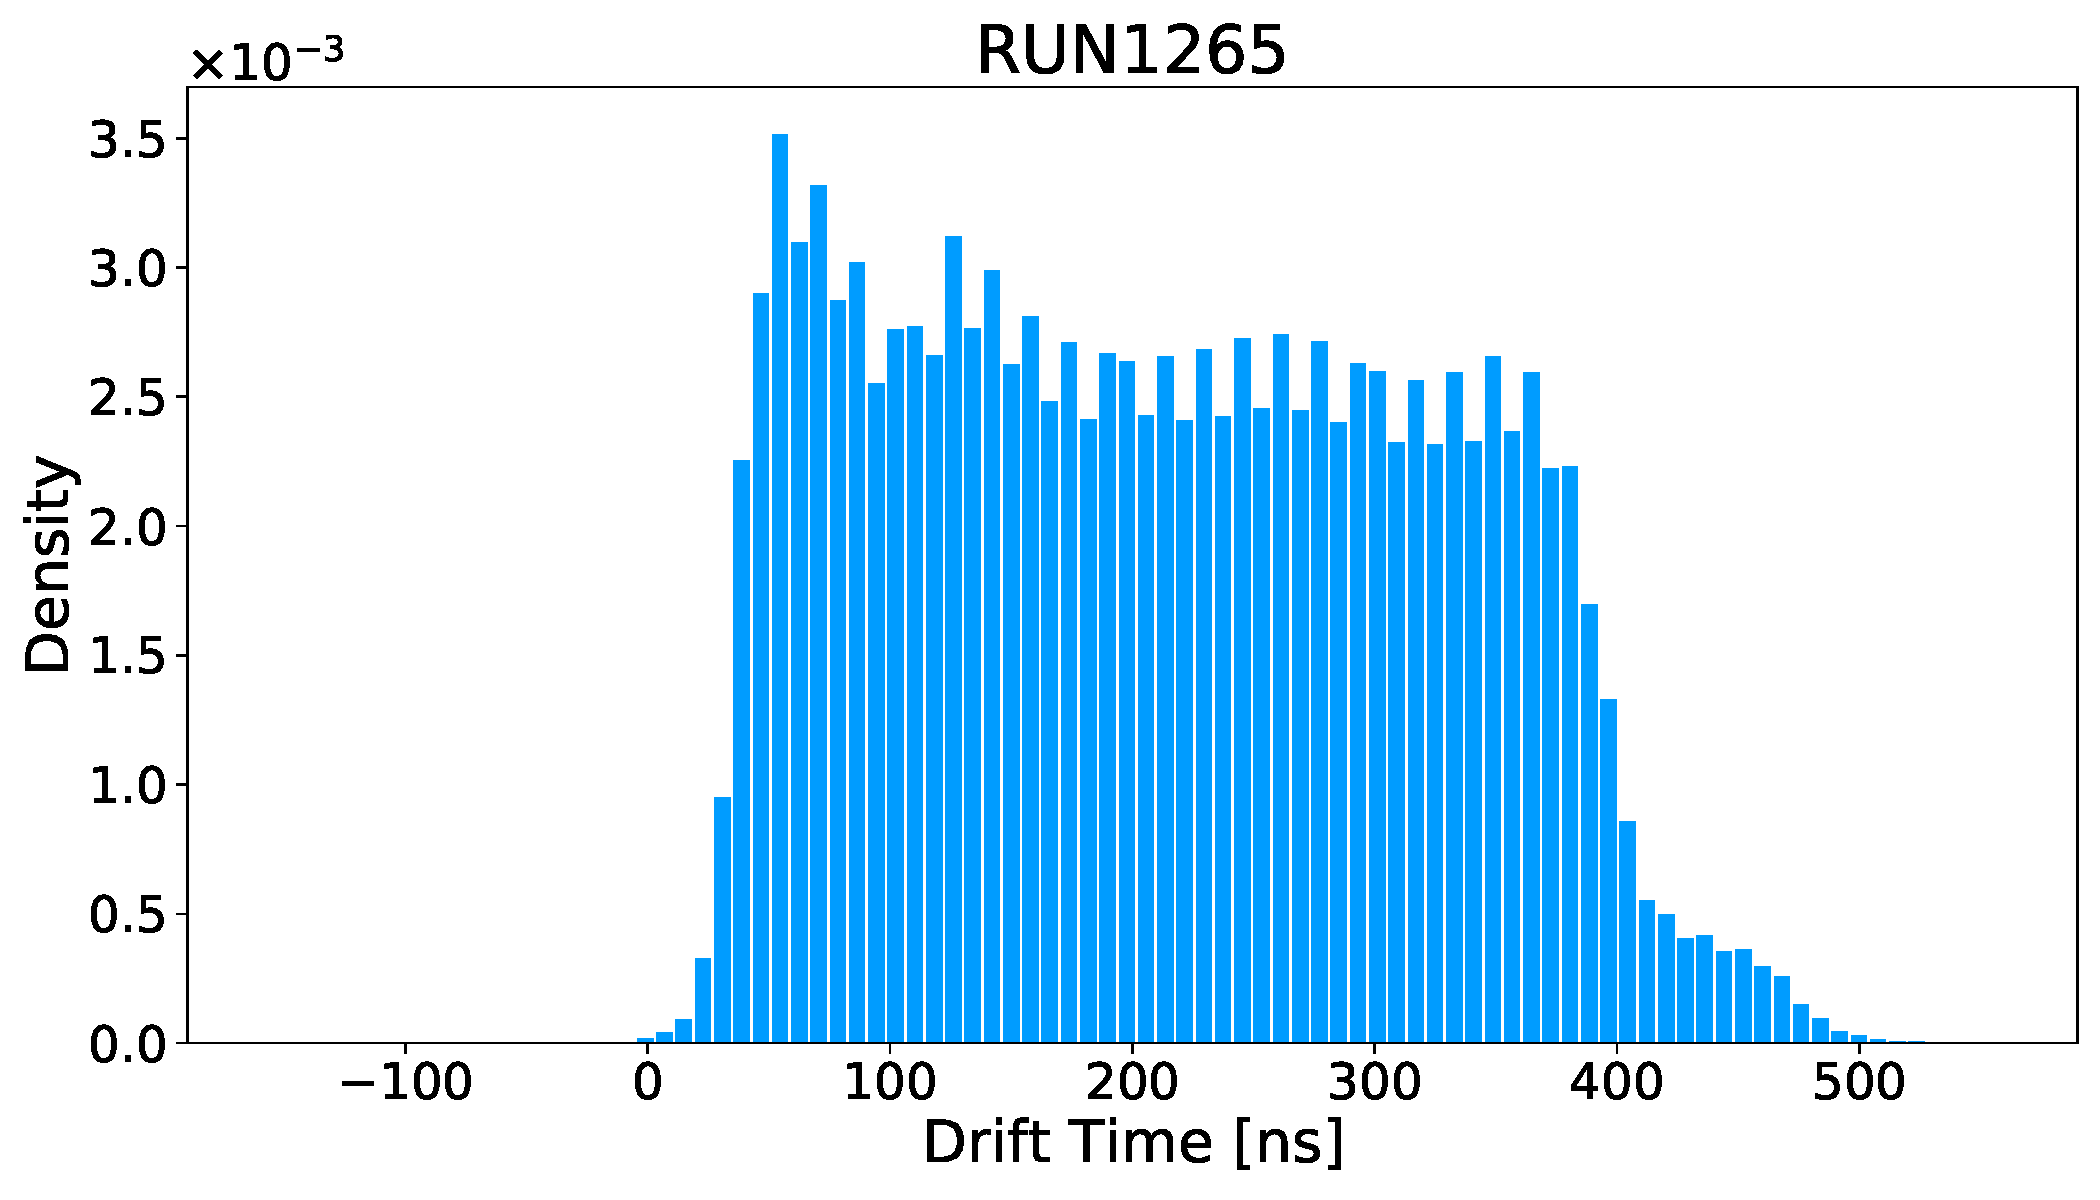
\includegraphics[width=1.0\textwidth]{./Images/1265_blue.pdf}
					\end{figure}

			\end{column}


			% RIGHT COLUMN
			\begin{column}{0.5\textwidth}

					\begin{figure}
						\centering 
						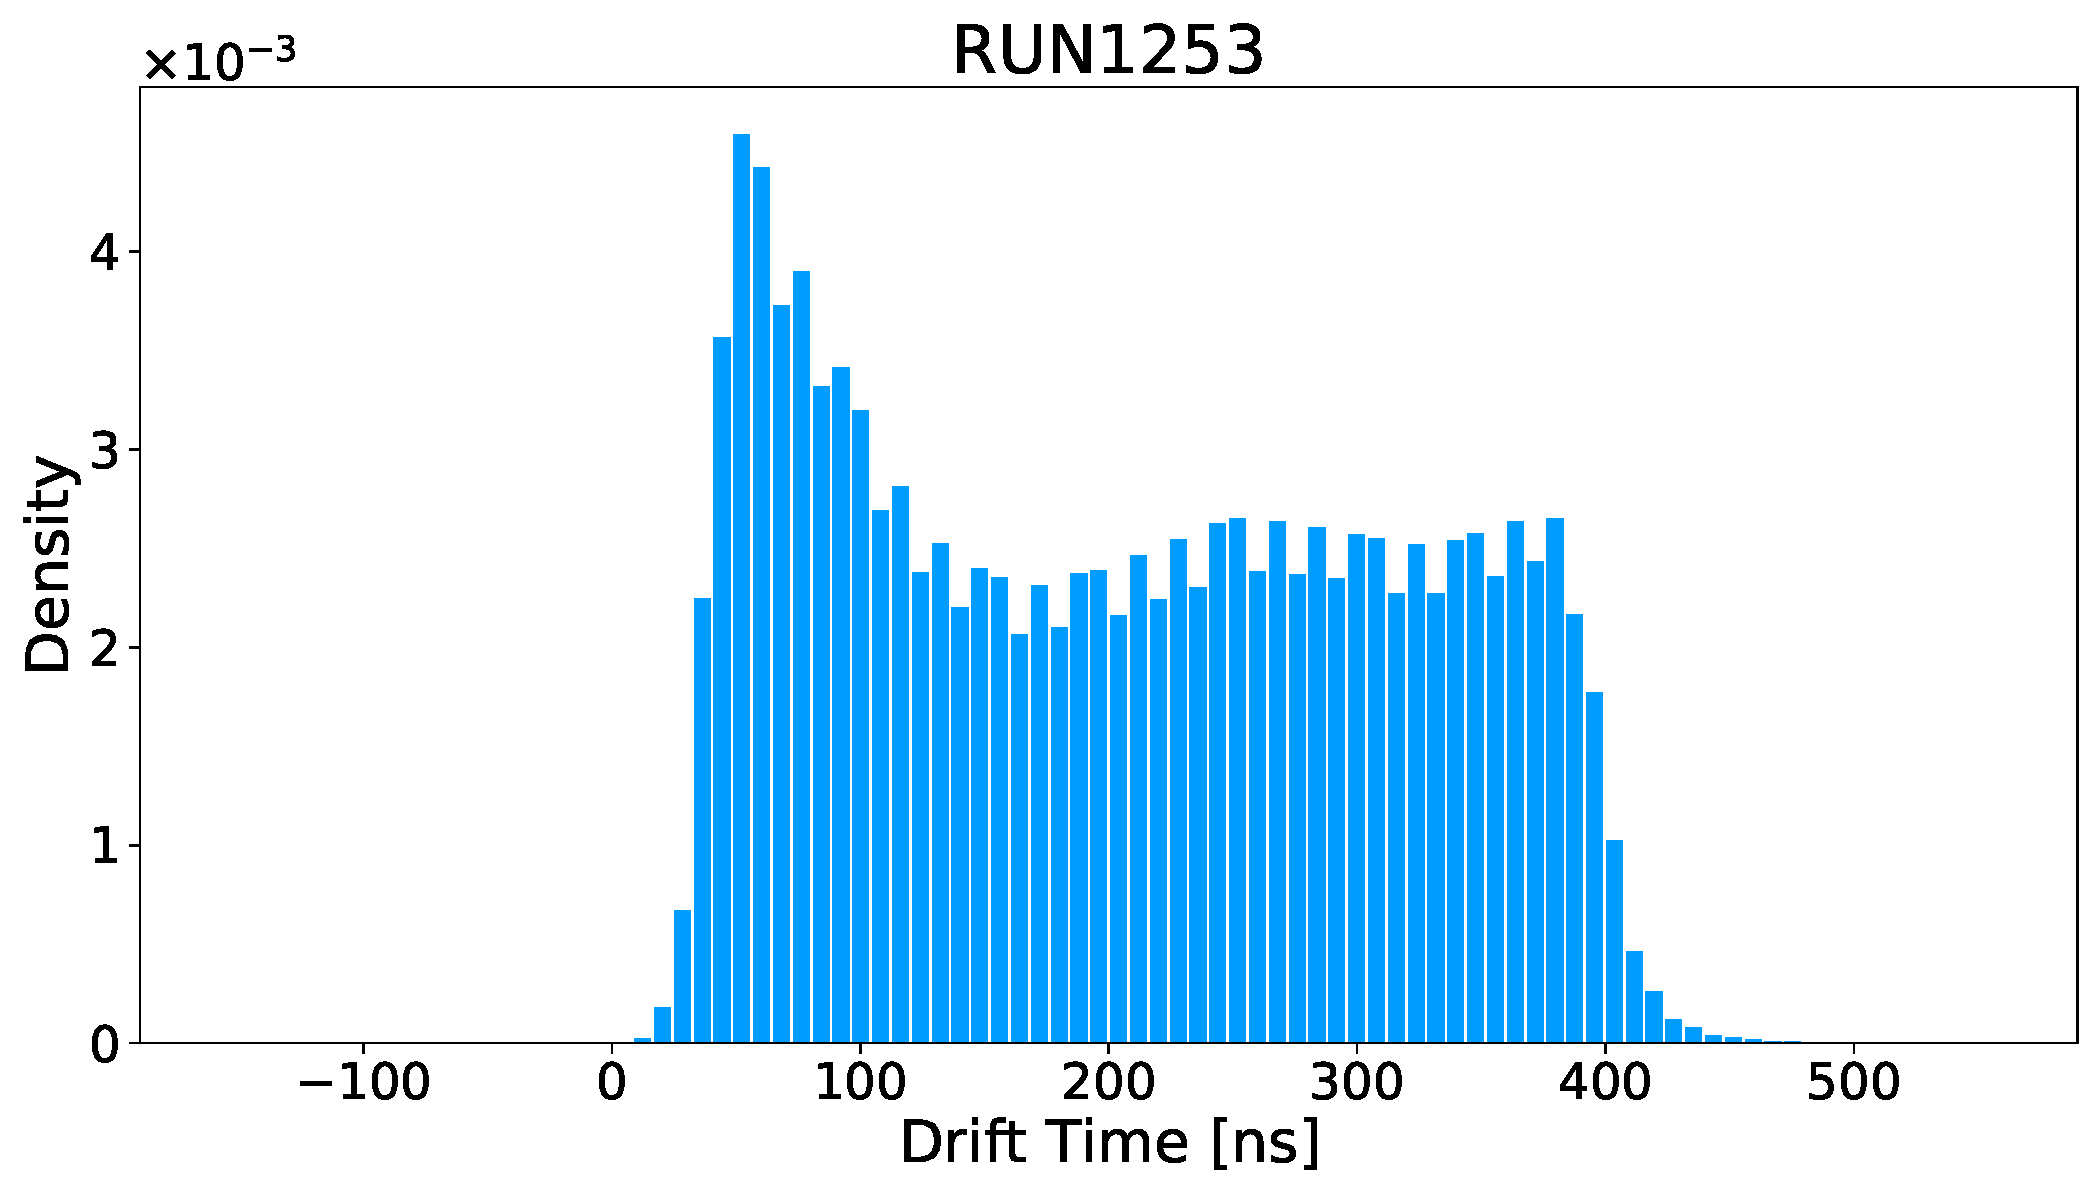
\includegraphics[width=1.0\textwidth]{./Images/1253_blue.pdf}
						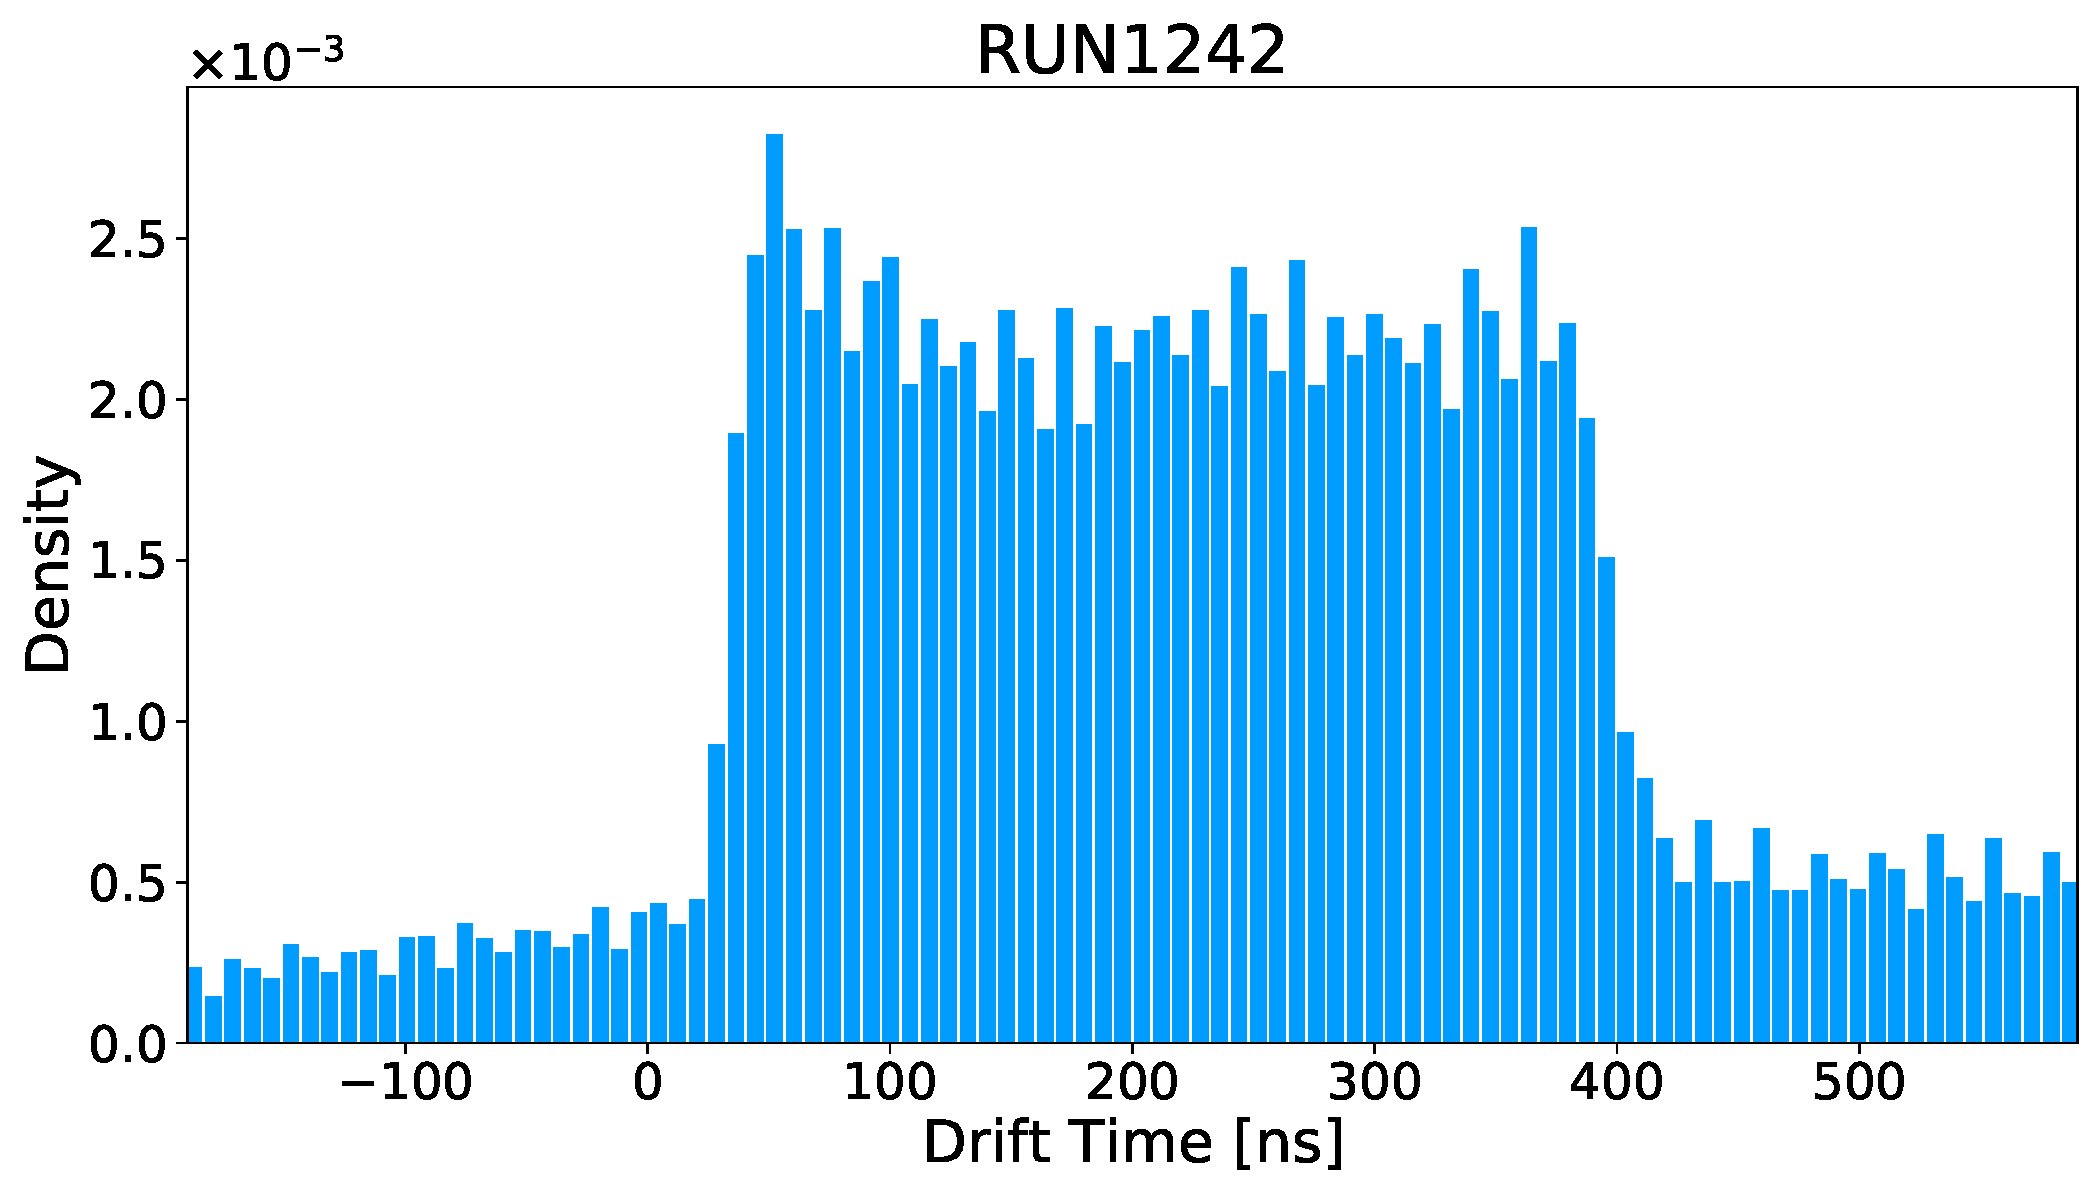
\includegraphics[width=1.0\textwidth]{./Images/1242_blue.pdf}
					\end{figure}

			\end{column}
		\end{columns}
		}<1>

		\only{
			\begin{columns}%[onlytextwidth]

			% LEFT COLUMN
			\begin{column}{0.5\textwidth}

					\begin{figure}
						\centering 
						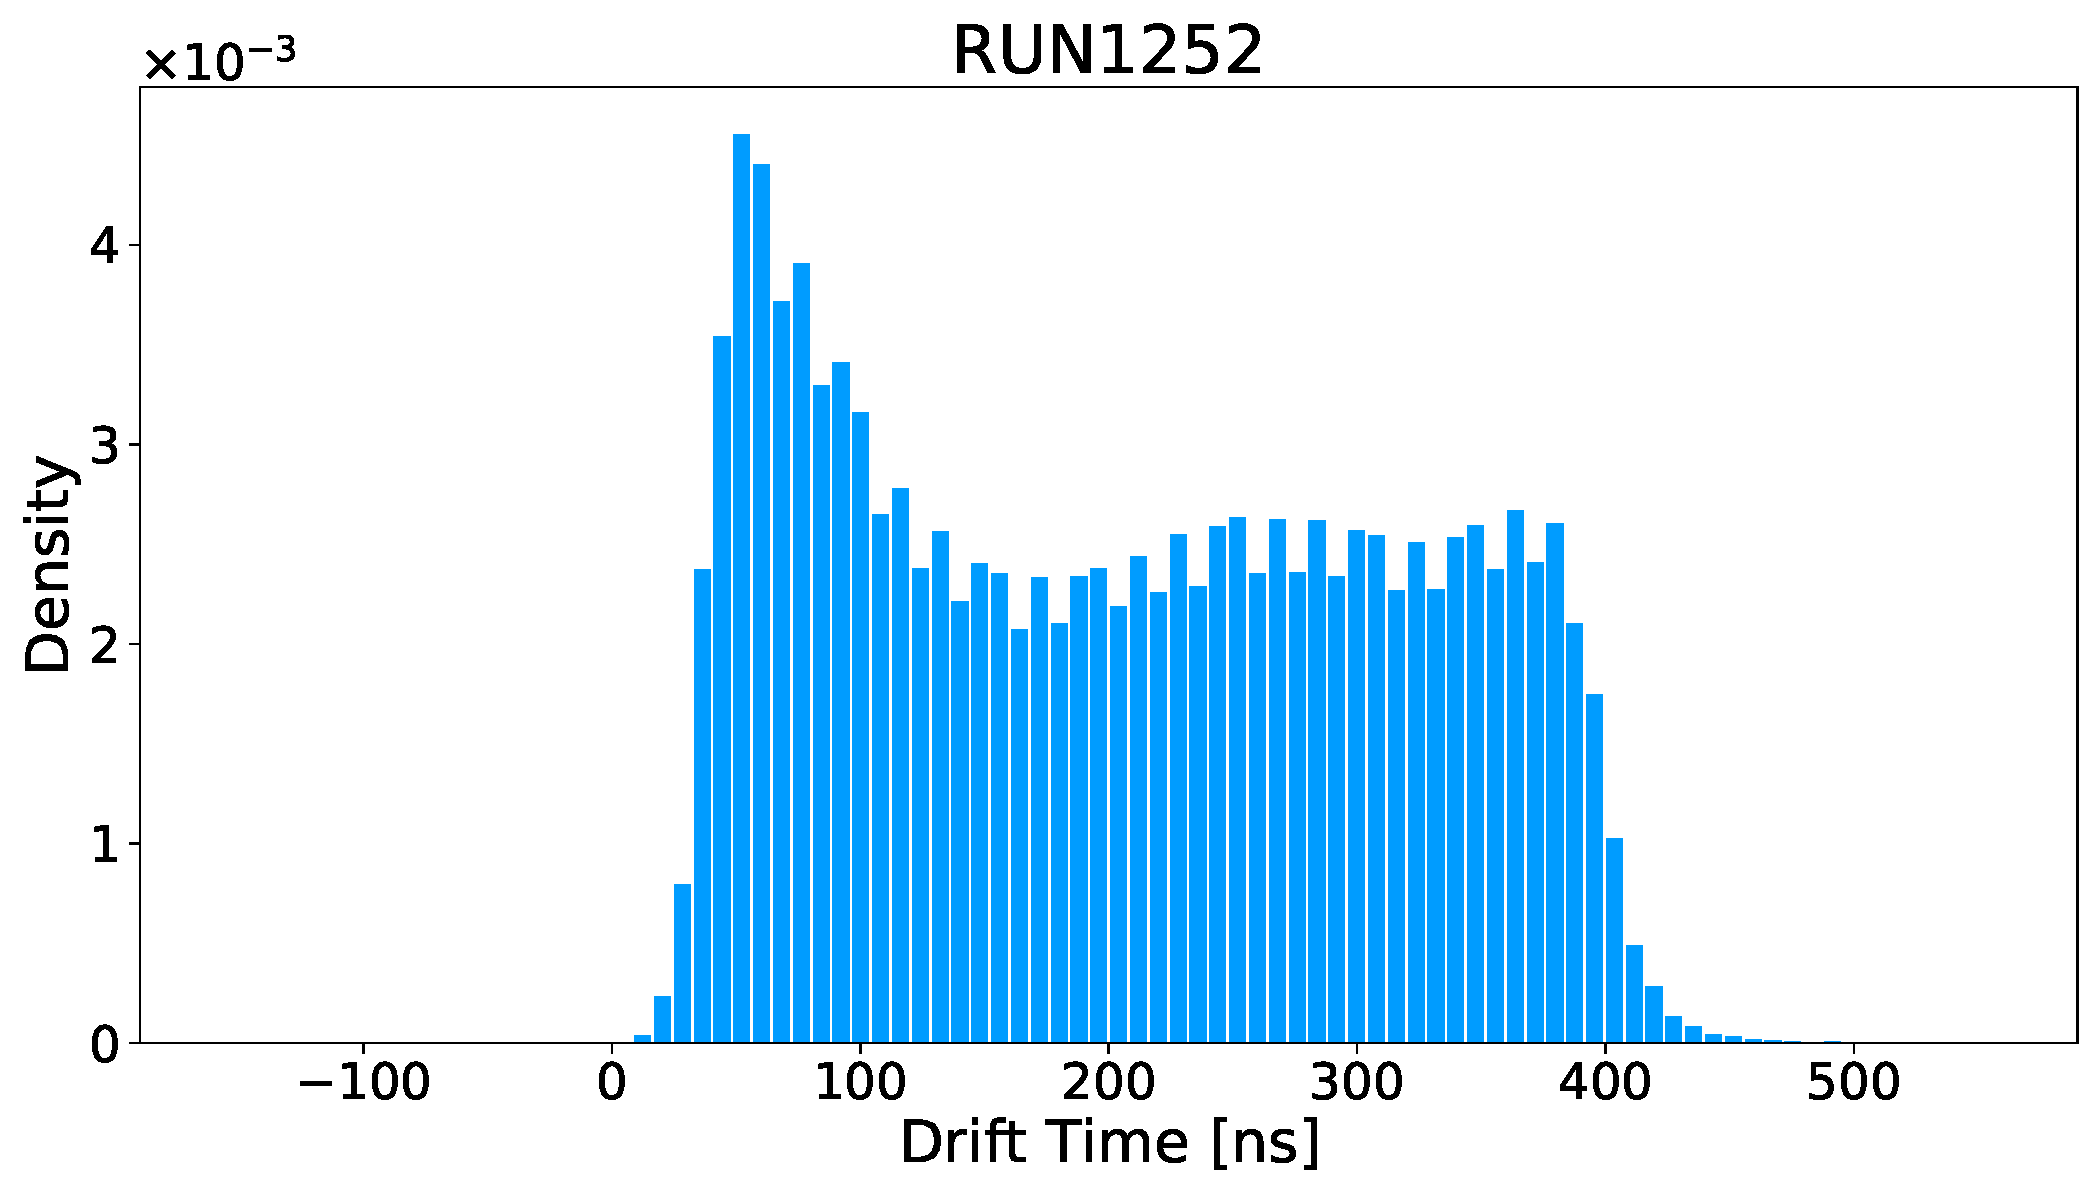
\includegraphics[width=1.0\textwidth]{./Images/reference_blue.pdf}
						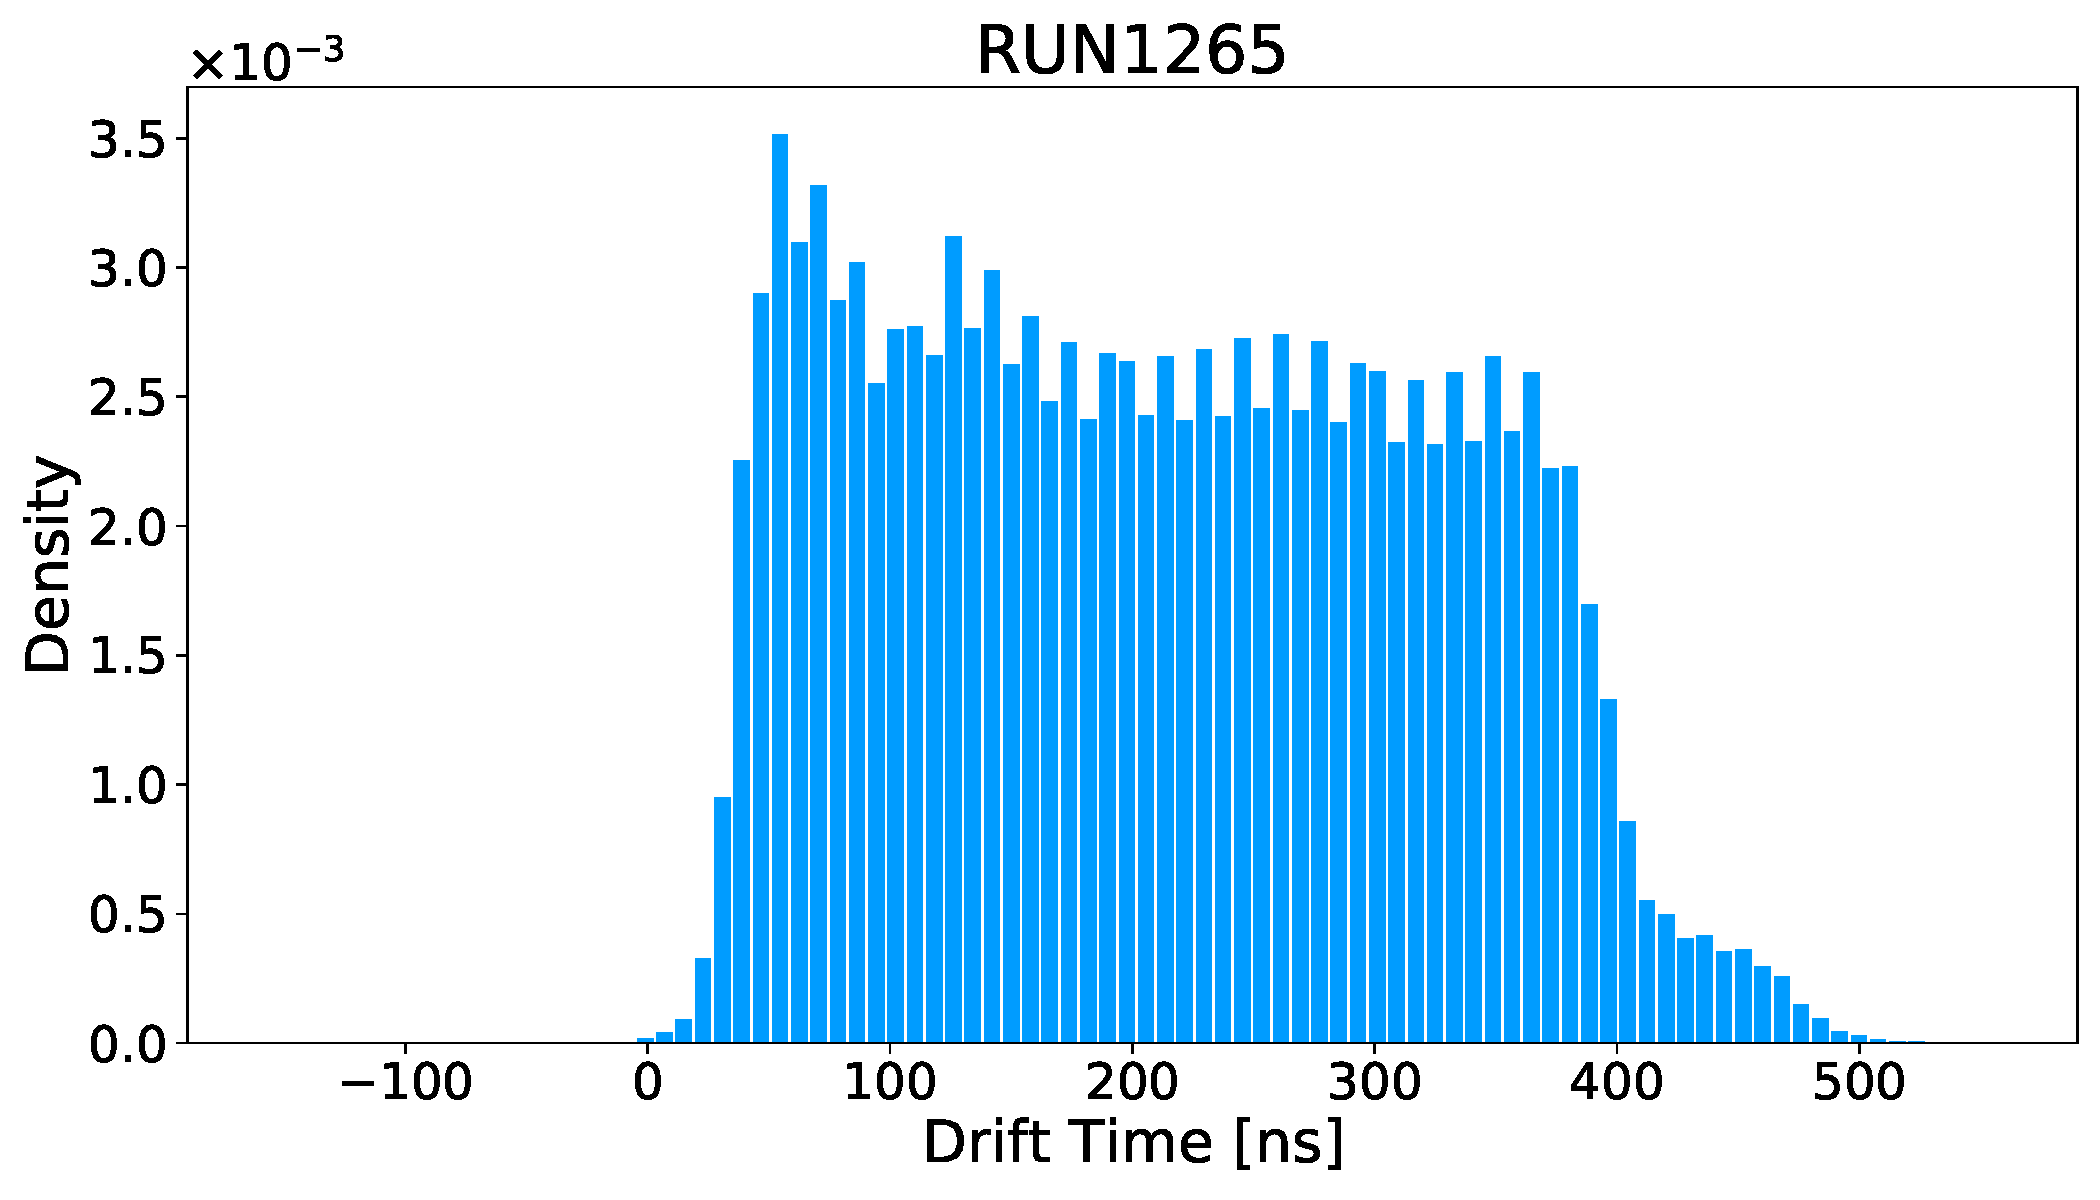
\includegraphics[width=1.0\textwidth]{./Images/1265_blue.pdf}
					\end{figure}

			\end{column}


			% RIGHT COLUMN
			\begin{column}{0.5\textwidth}

					\begin{figure}
						\centering 
						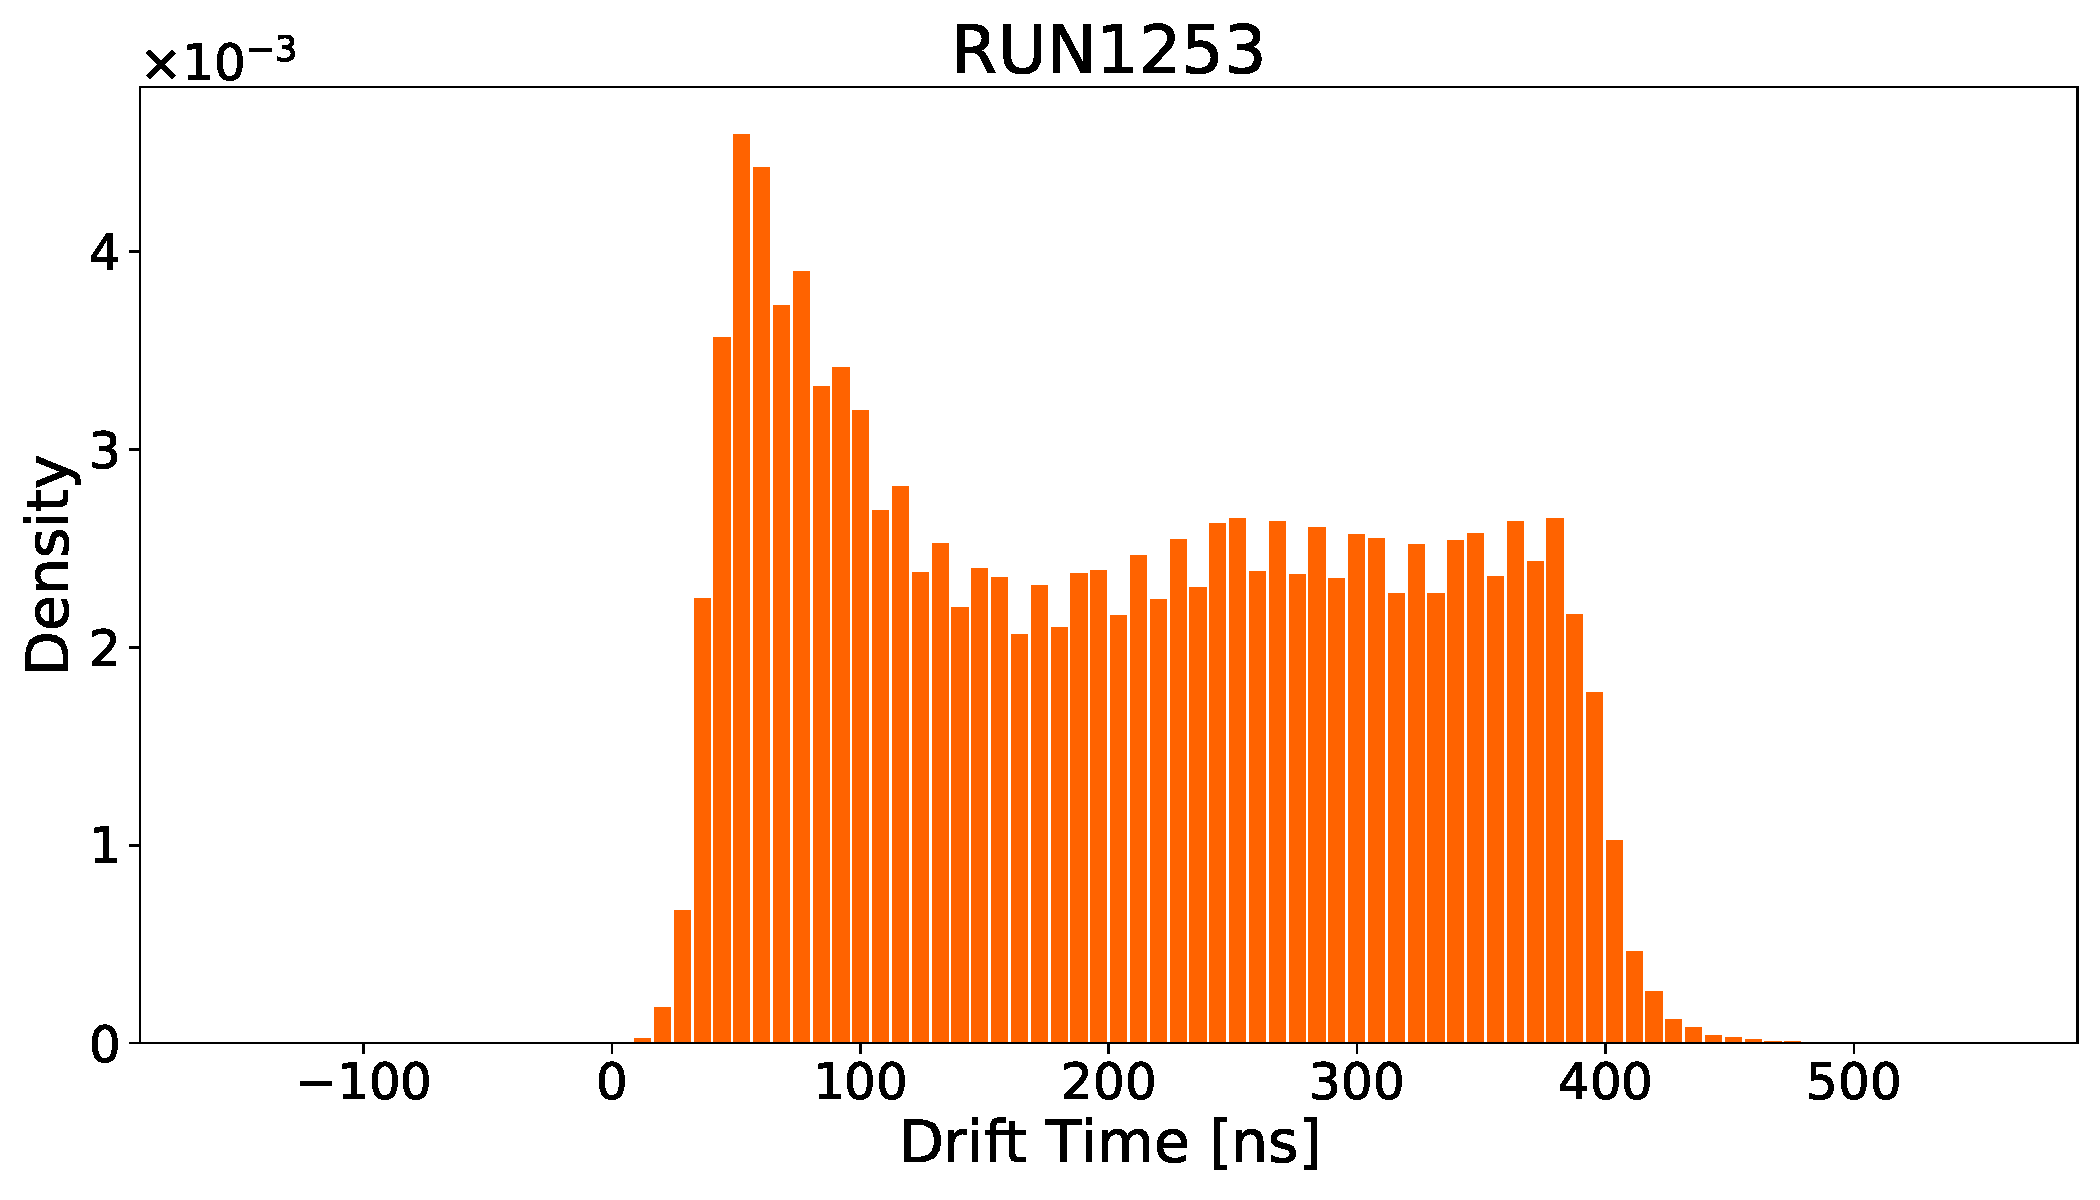
\includegraphics[width=1.0\textwidth]	{./Images/1253_orange.pdf}
						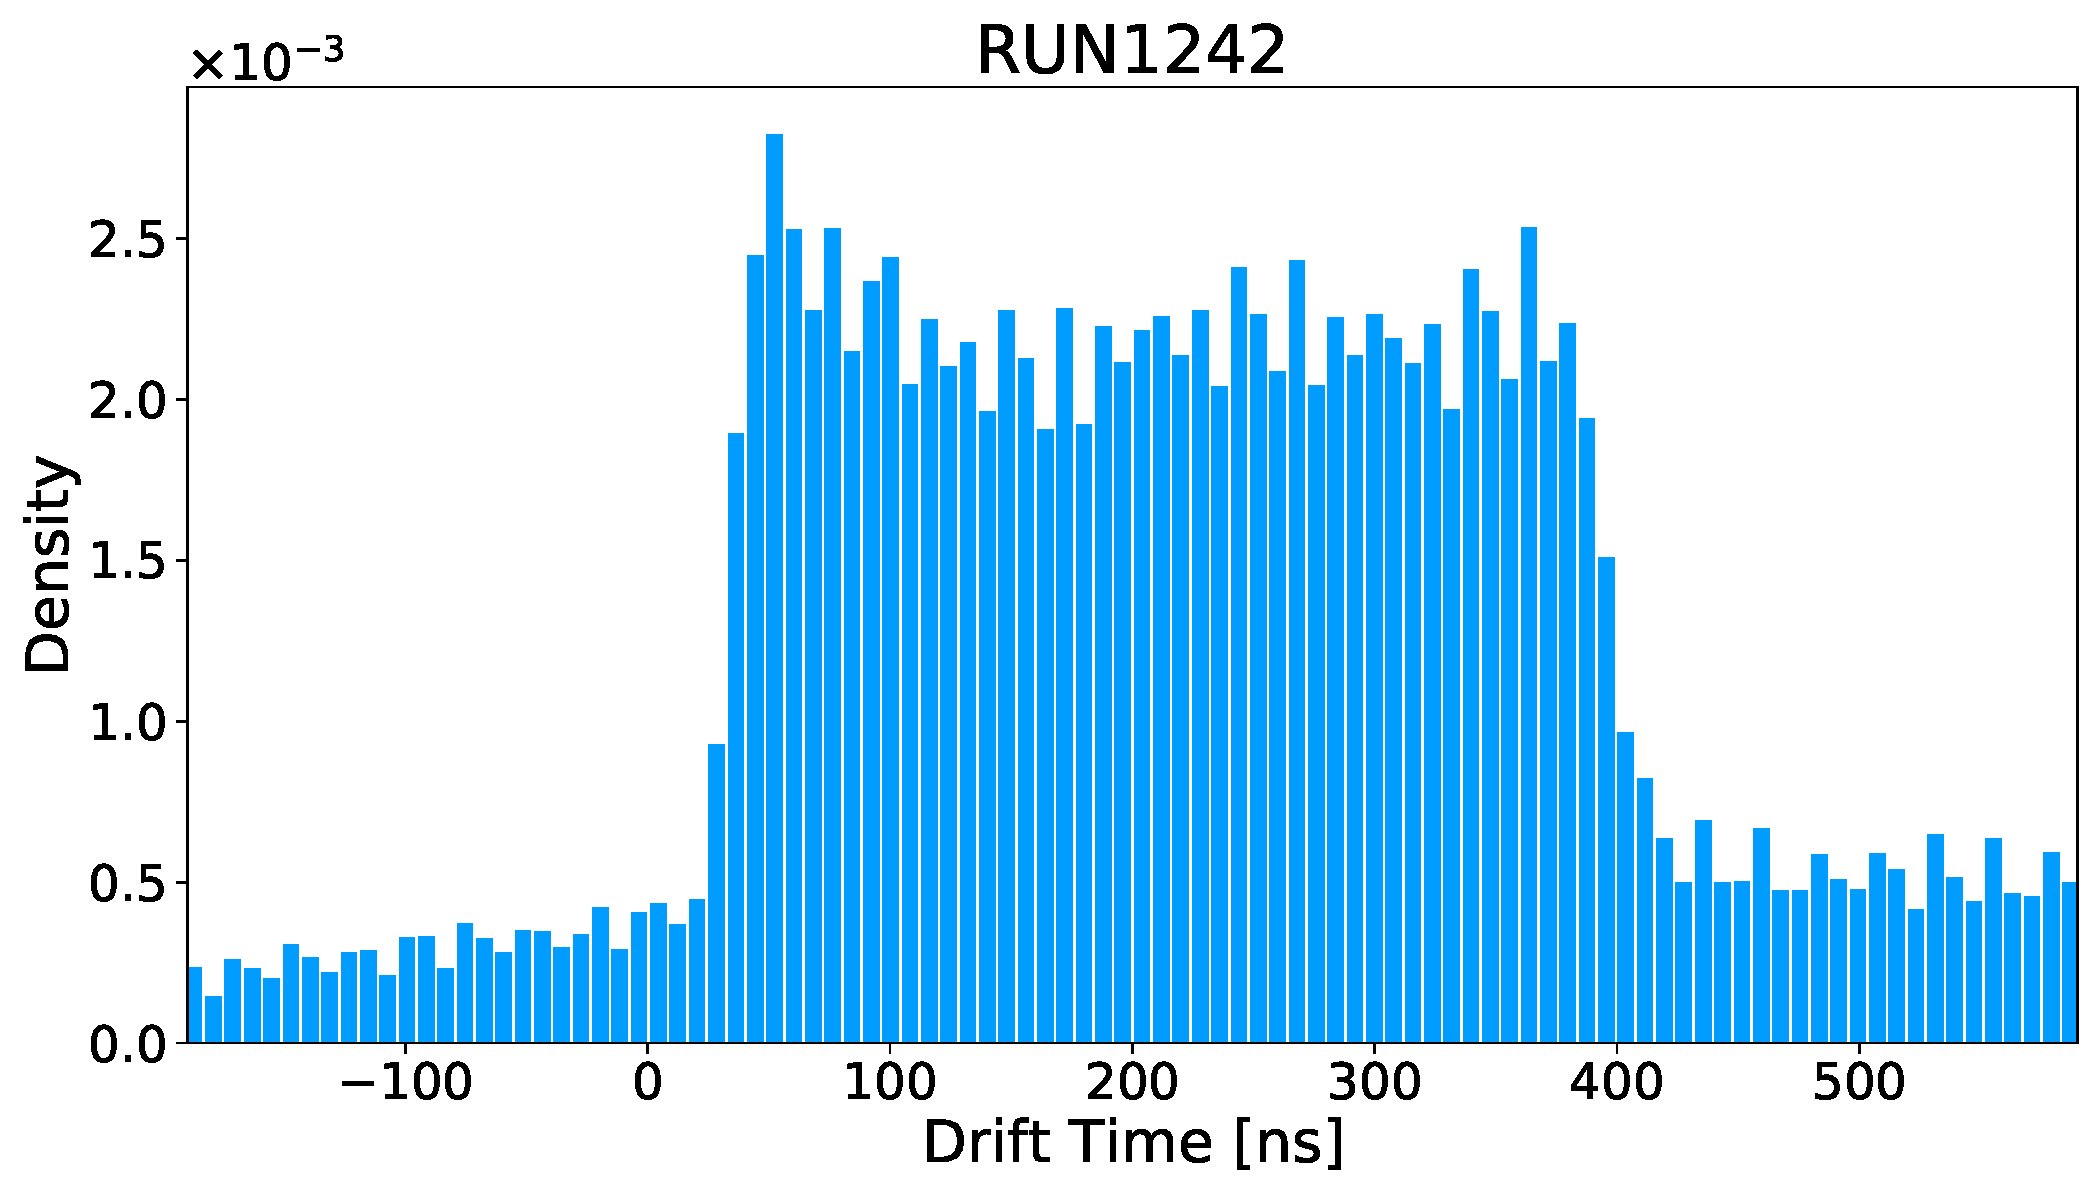
\includegraphics[width=1.0\textwidth]{./Images/1242_blue.pdf}
					\end{figure}

			\end{column}
		\end{columns}
		}<2>

		\only{
			\begin{columns}%[onlytextwidth]

			% LEFT COLUMN
			\begin{column}{0.5\textwidth}

					\begin{figure}
						\centering 
						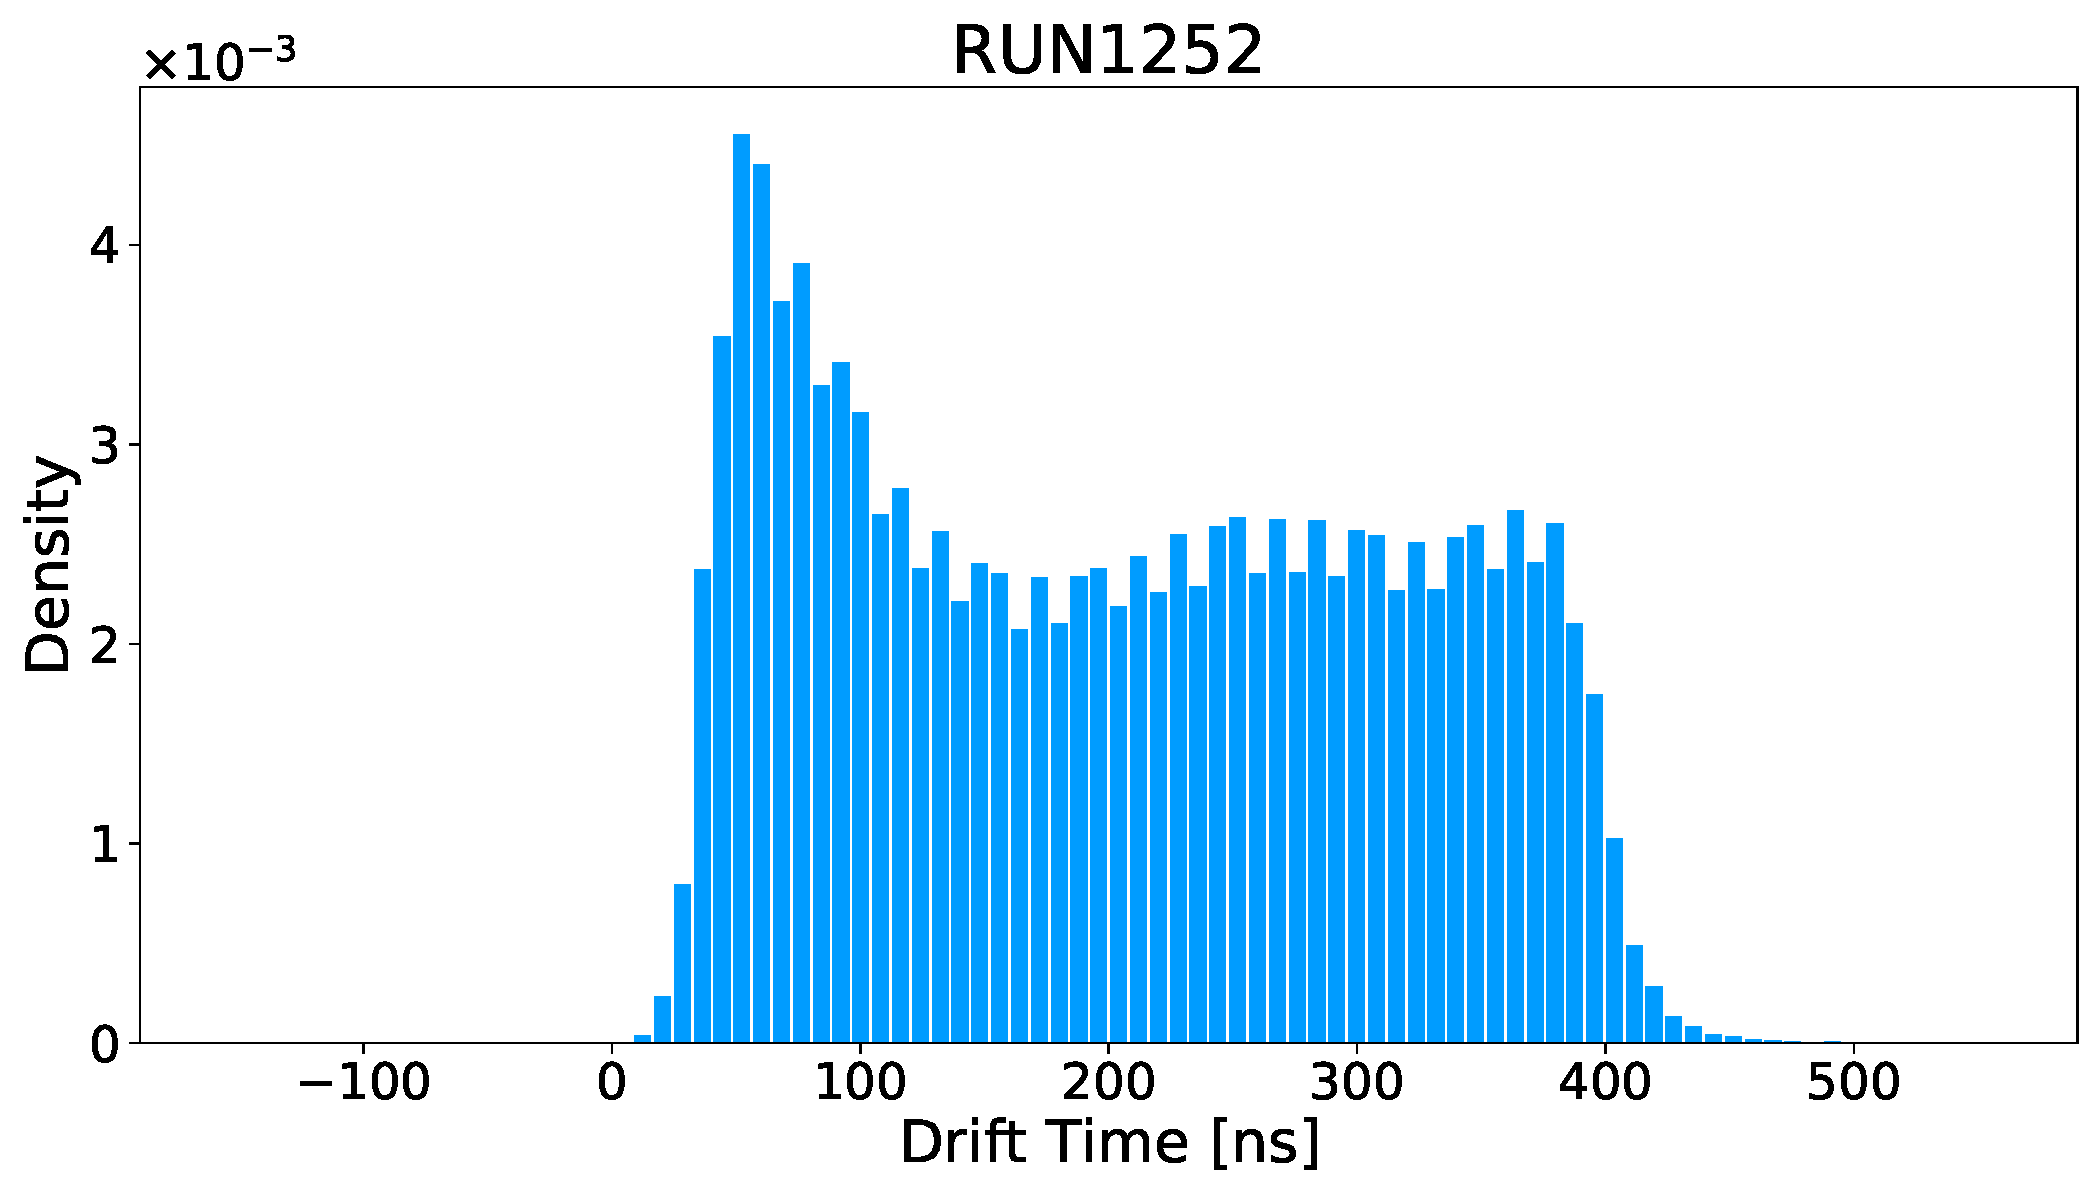
\includegraphics[width=1.0\textwidth]{./Images/reference_blue.pdf}
						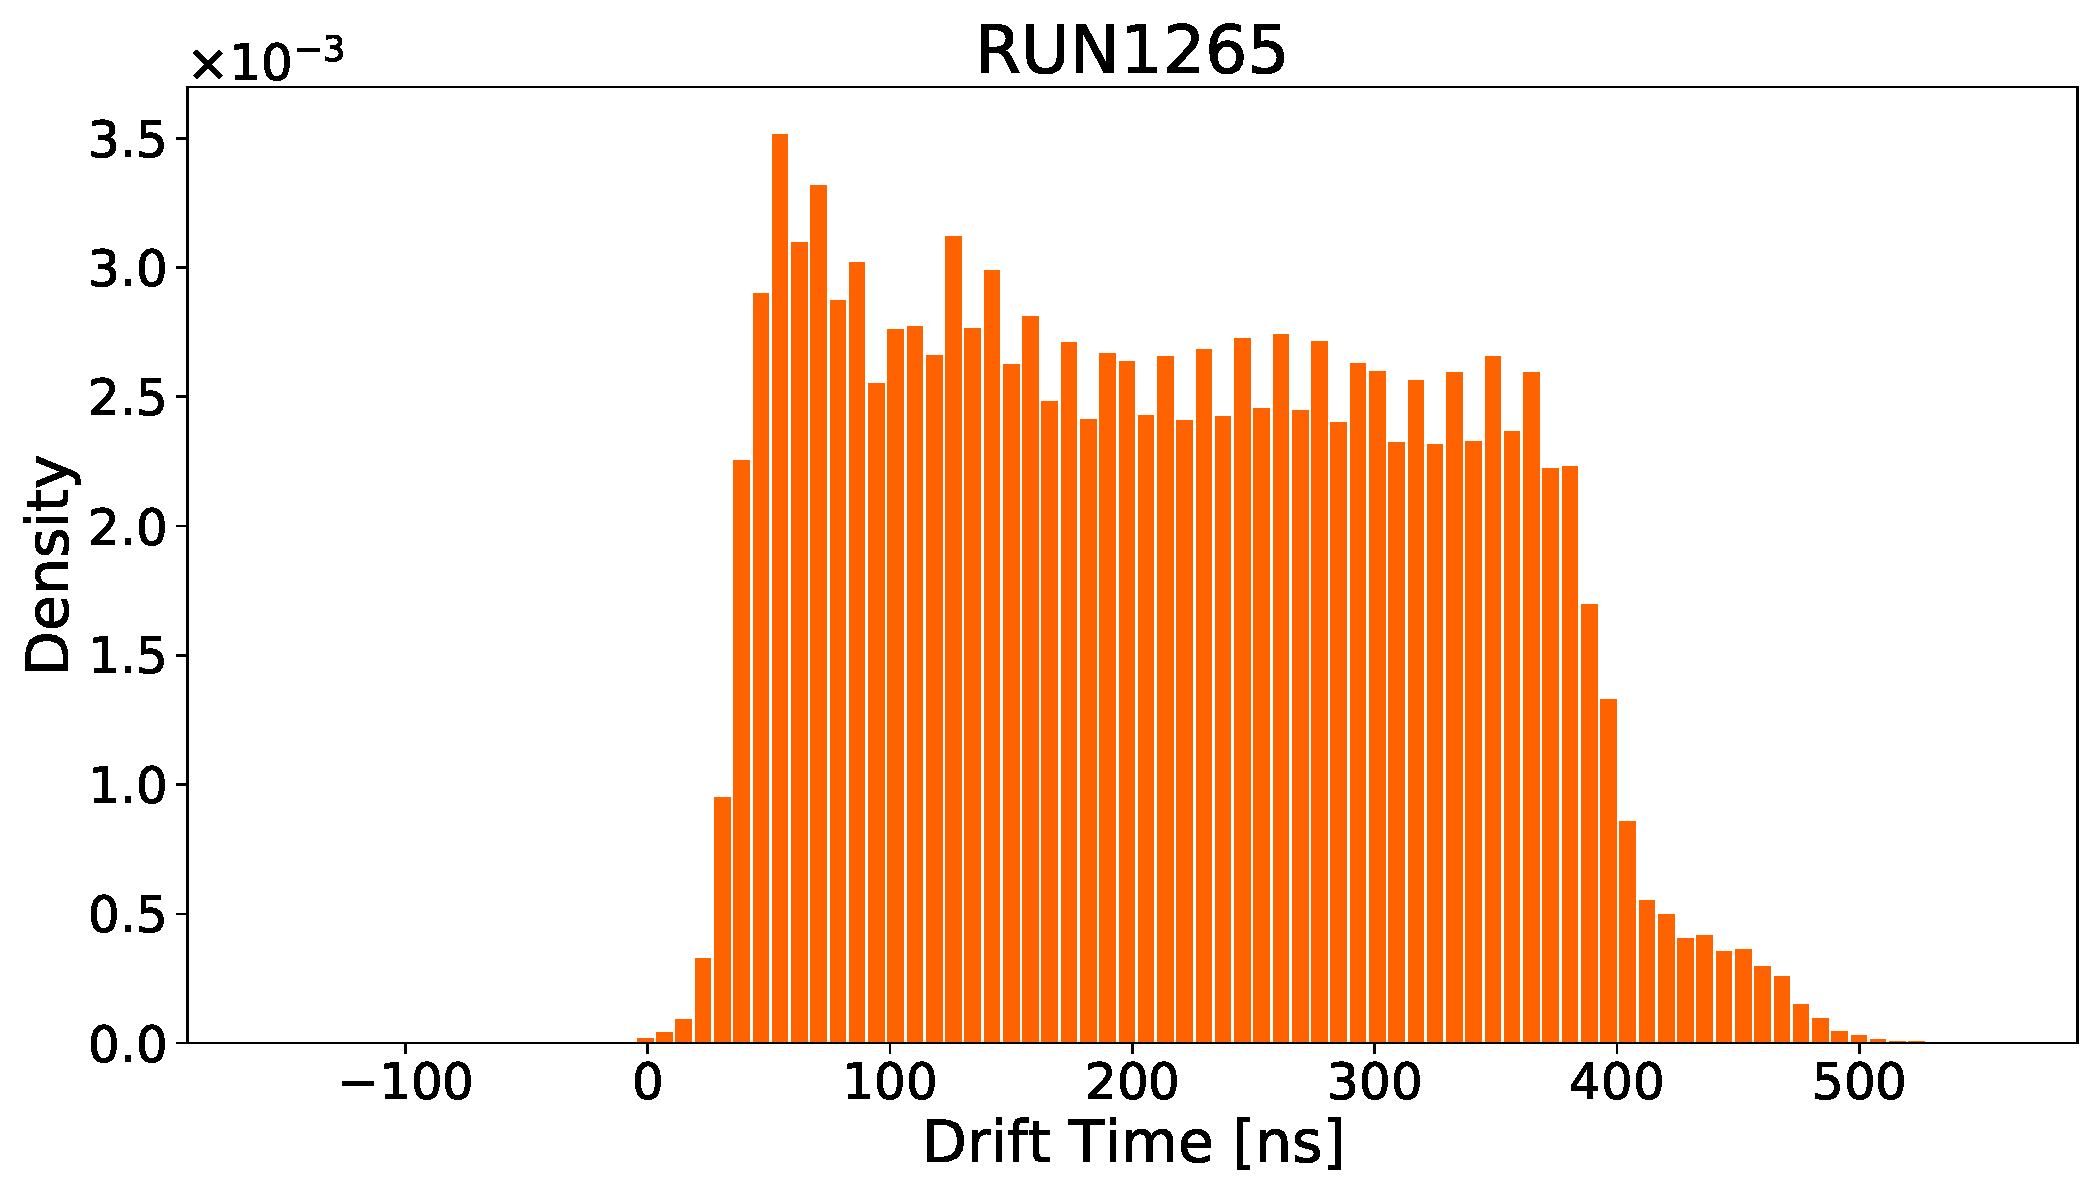
\includegraphics[width=1.0\textwidth]	{./Images/1265_orange.pdf}
					\end{figure}

			\end{column}


			% RIGHT COLUMN
			\begin{column}{0.5\textwidth}

					\begin{figure}
						\centering 
						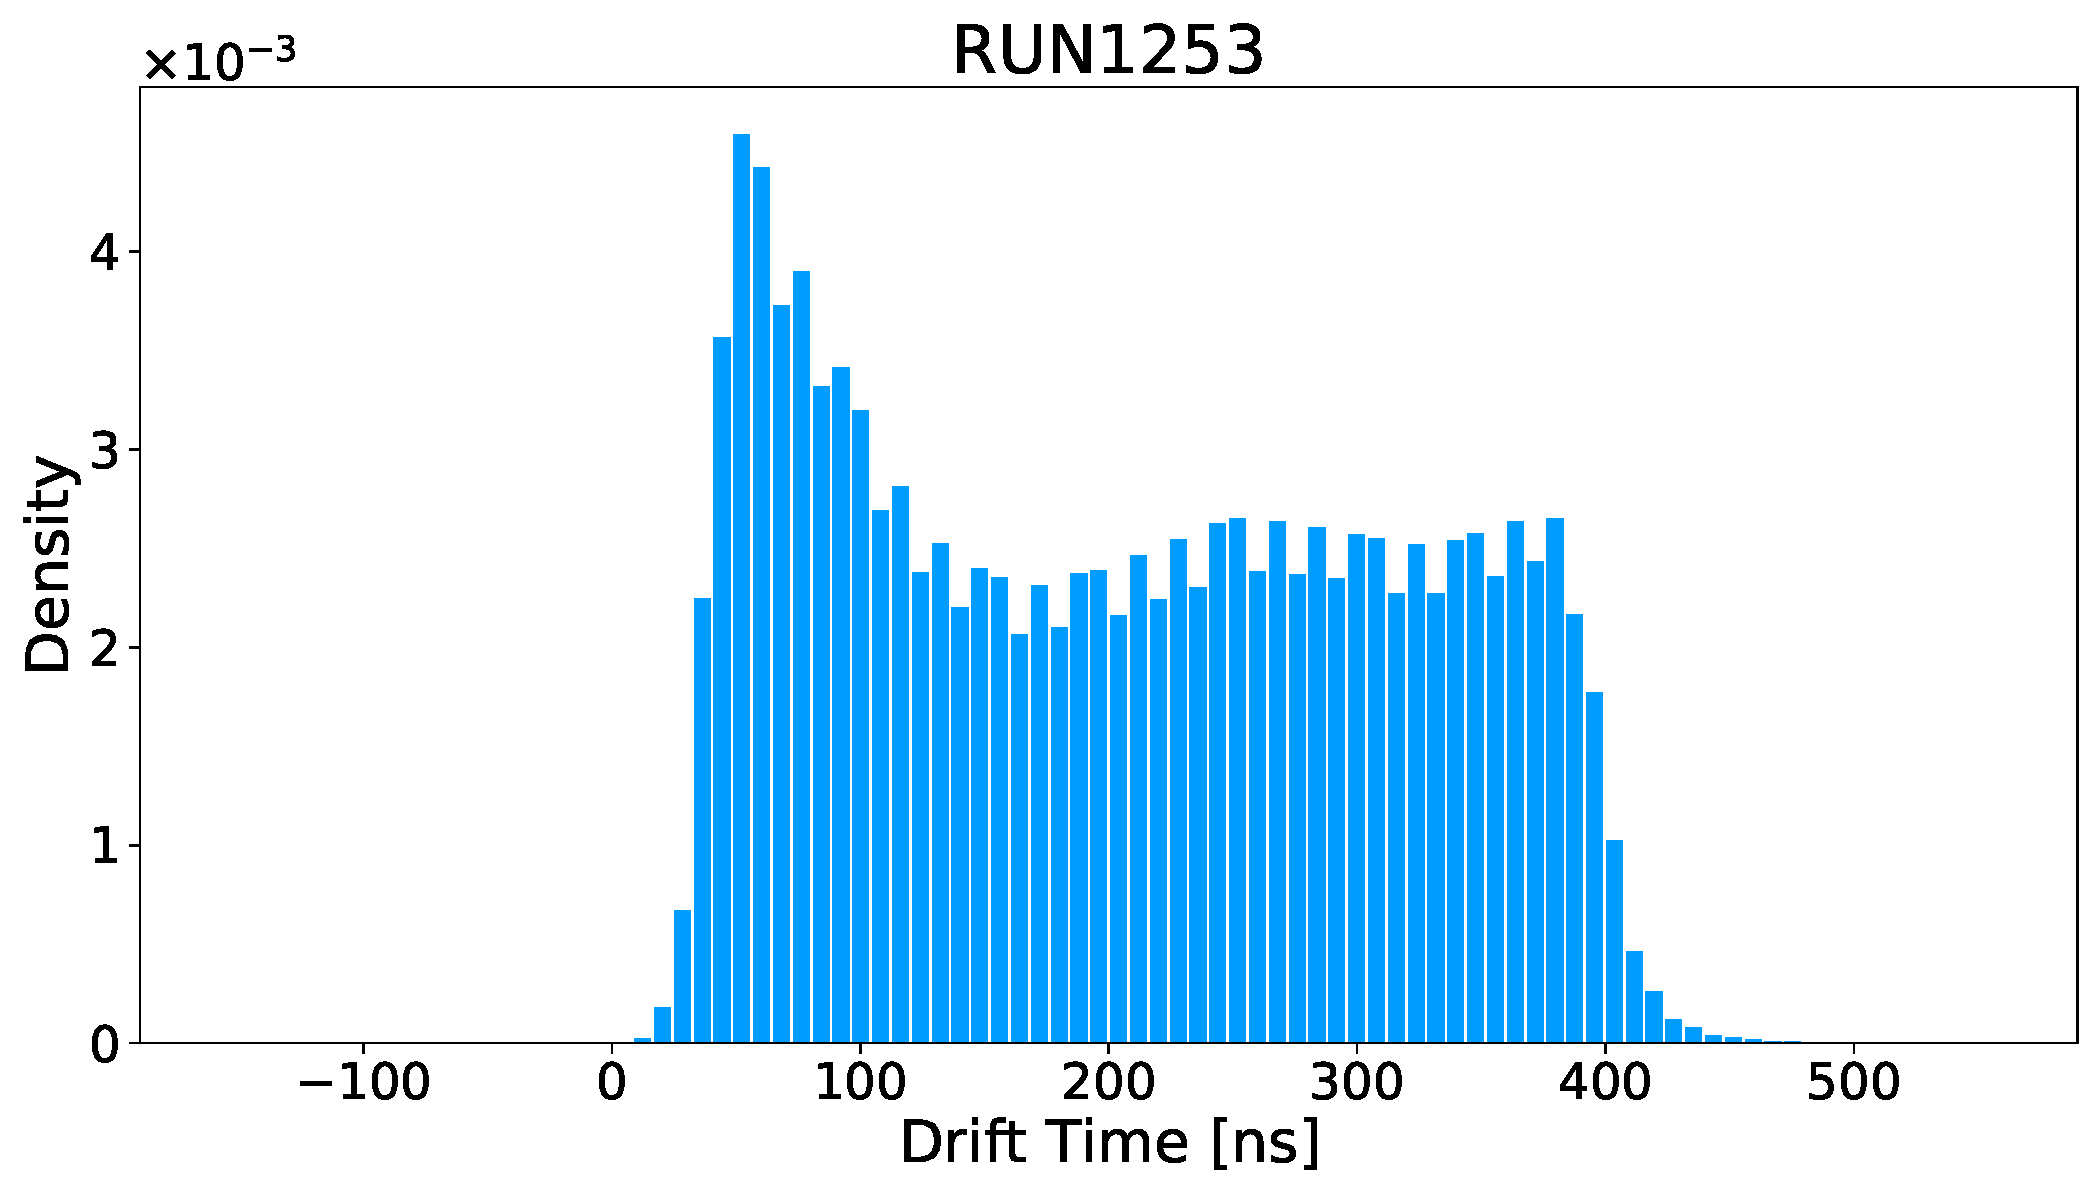
\includegraphics[width=1.0\textwidth]{./Images/1253_blue.pdf}
						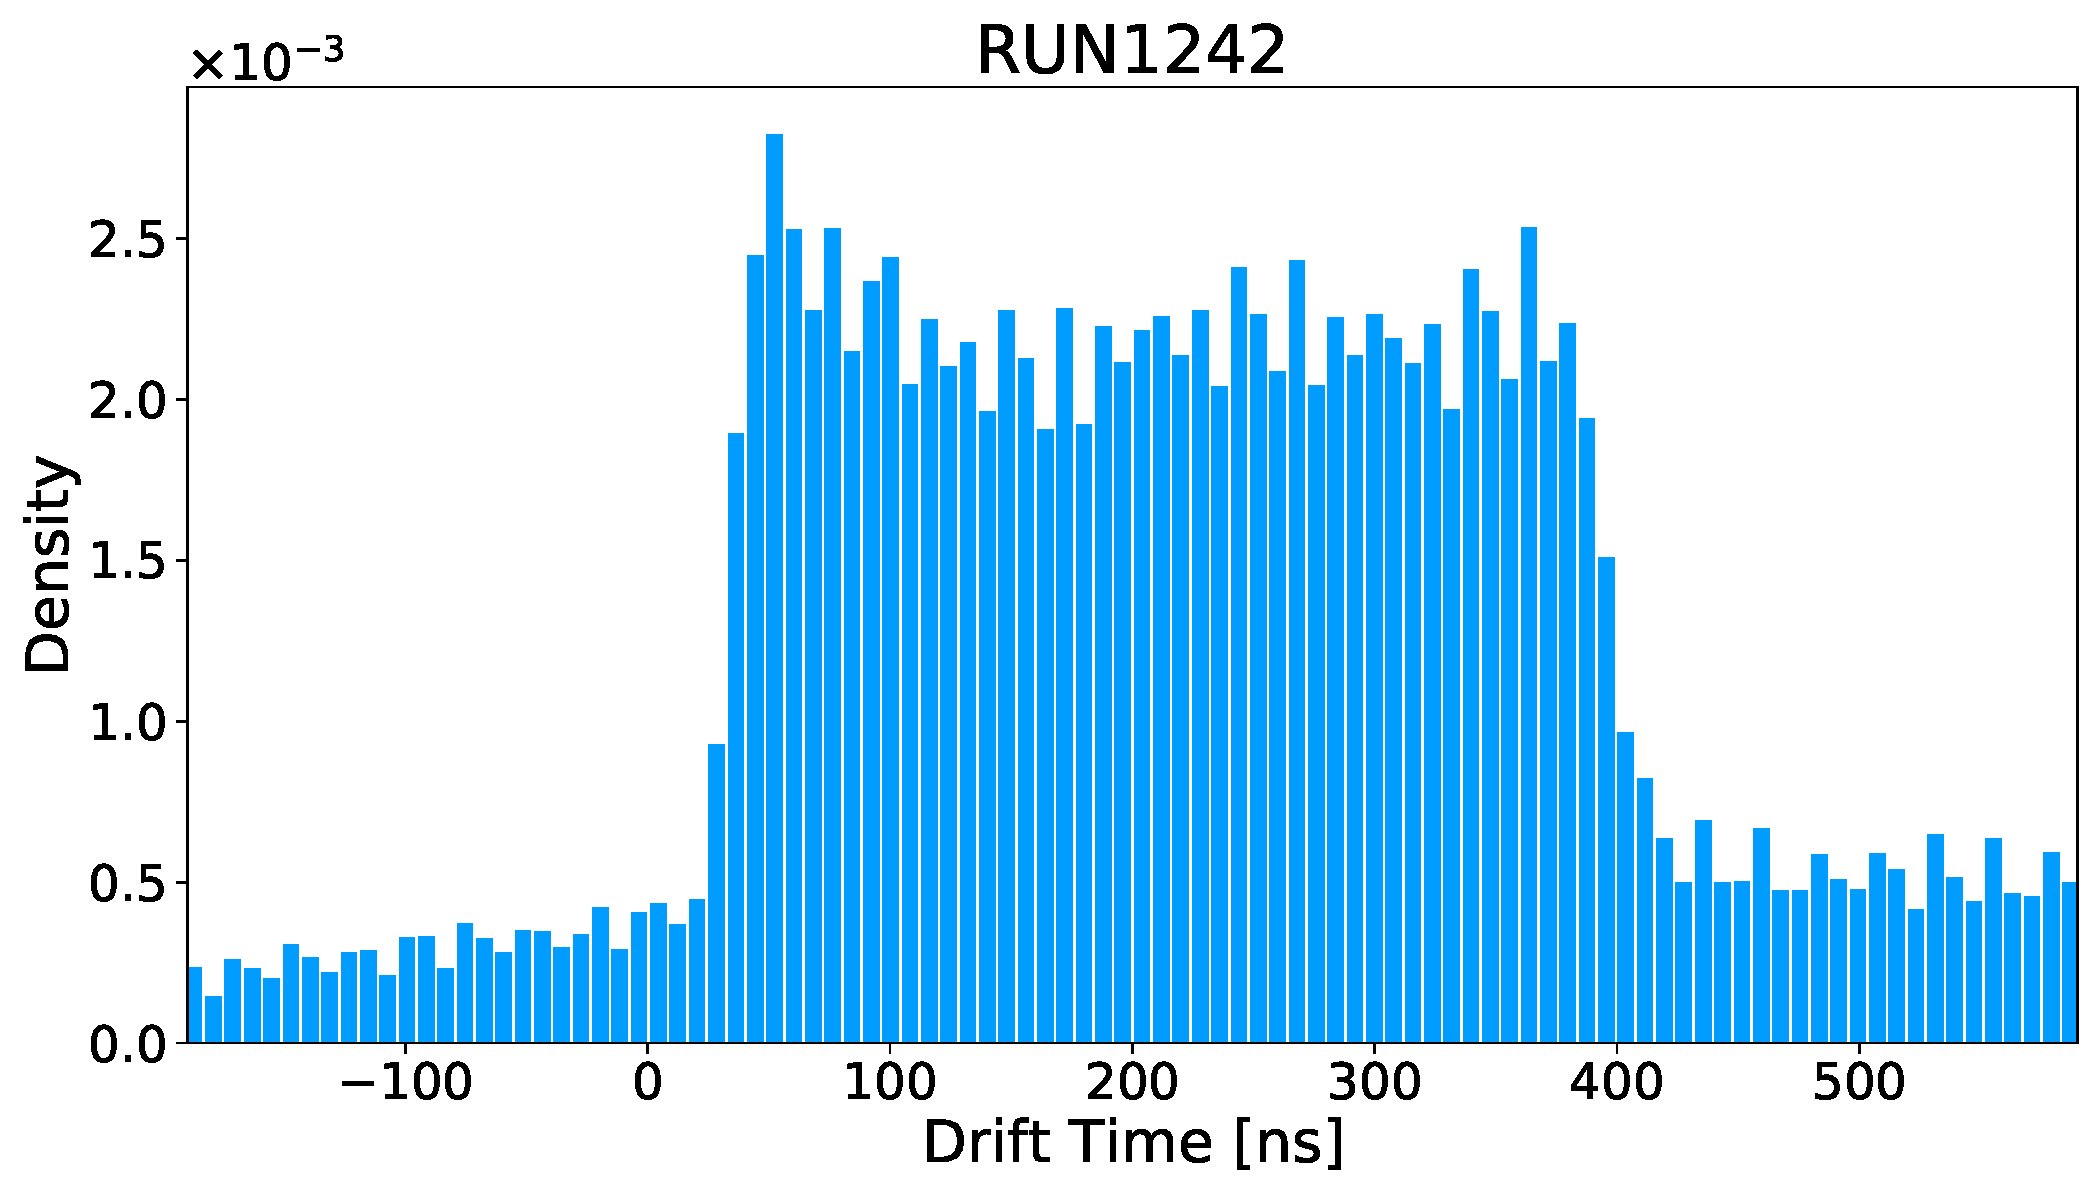
\includegraphics[width=1.0\textwidth]{./Images/1242_blue.pdf}
					\end{figure}

			\end{column}
		\end{columns}
		}<3>

		\only{
			\begin{columns}%[onlytextwidth]

			% LEFT COLUMN
			\begin{column}{0.5\textwidth}

					\begin{figure}
						\centering 
						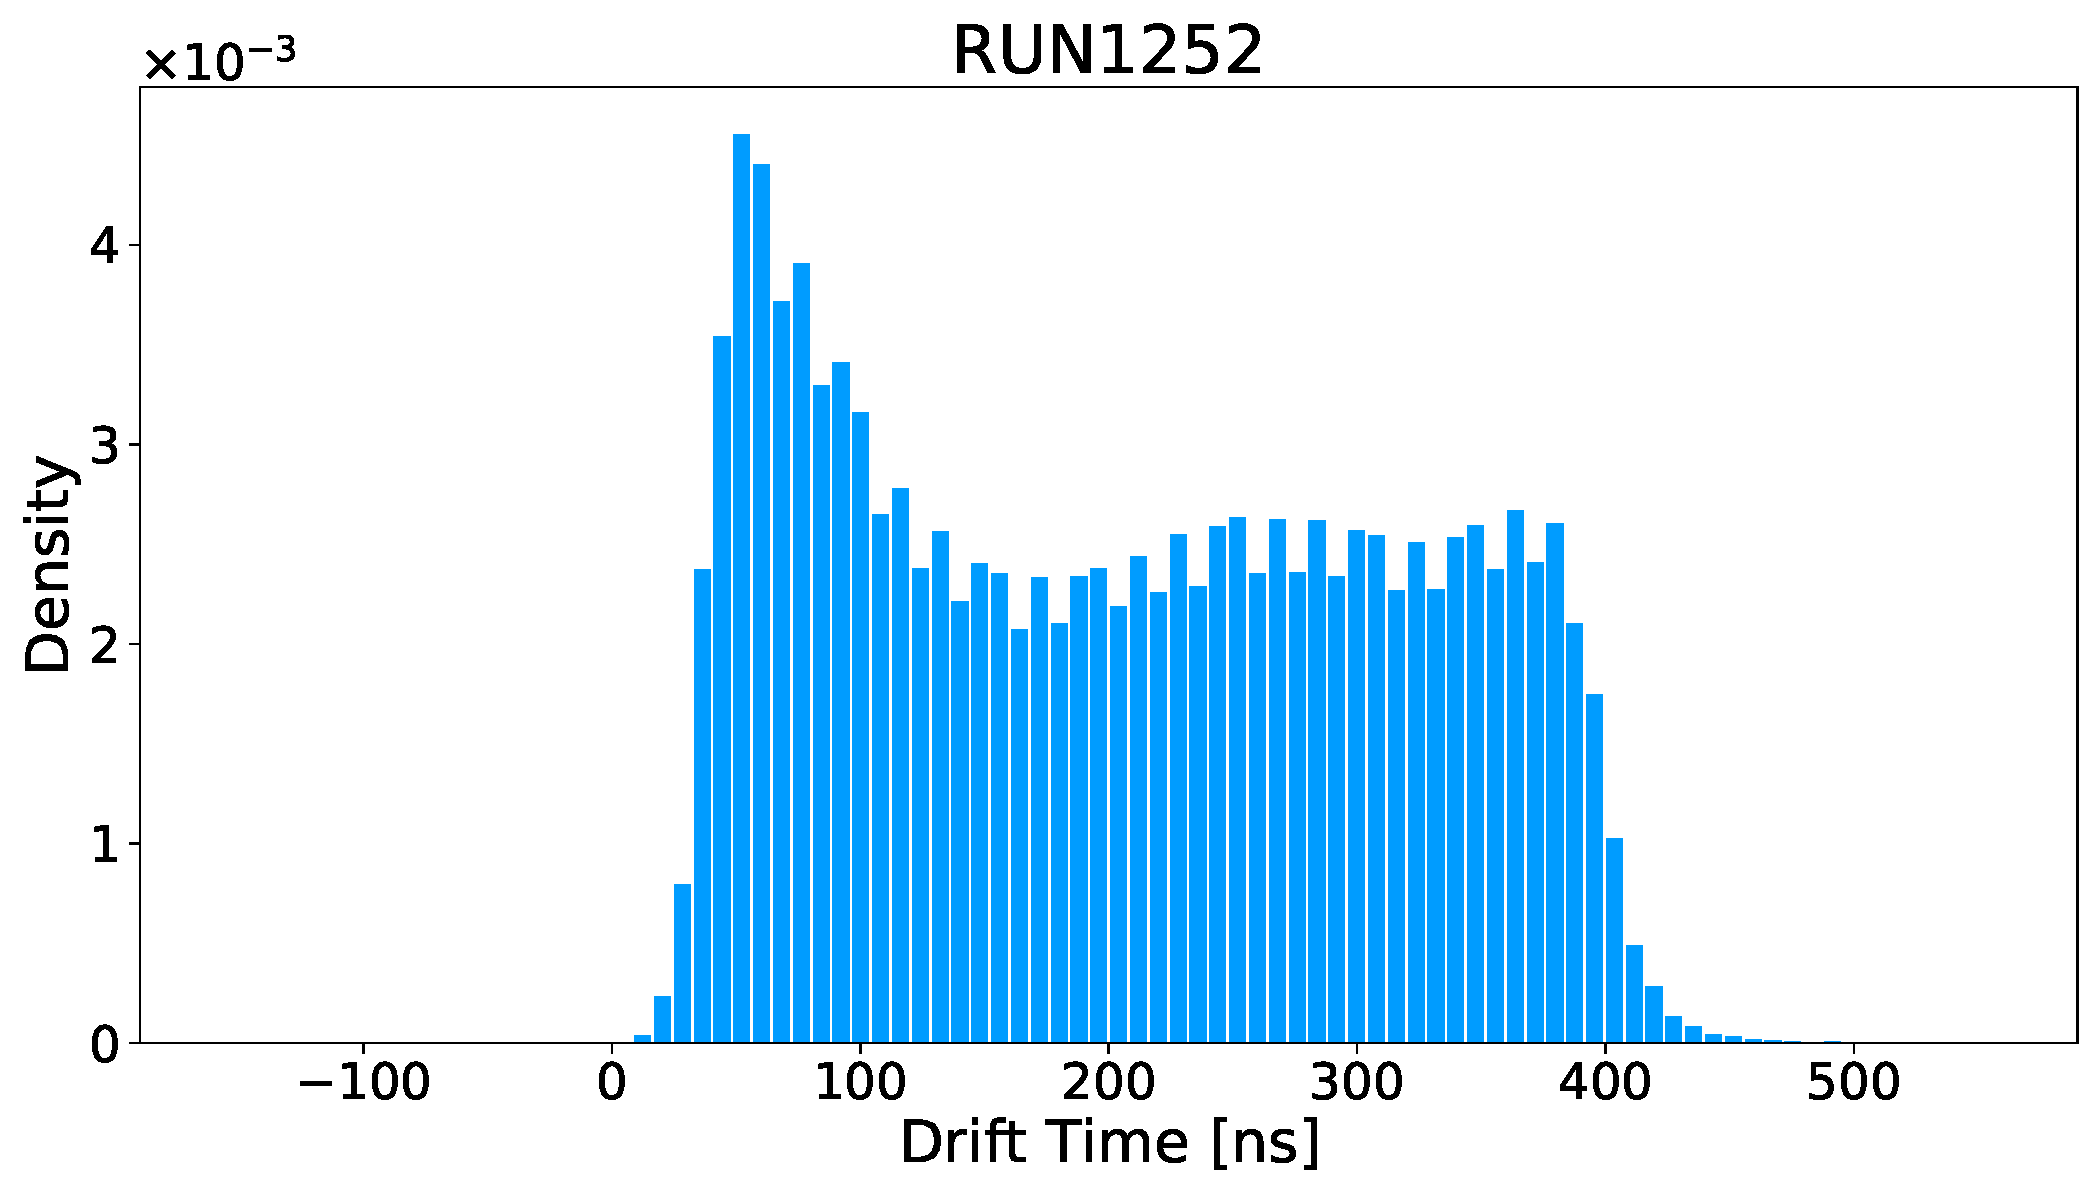
\includegraphics[width=1.0\textwidth]{./Images/reference_blue.pdf}
						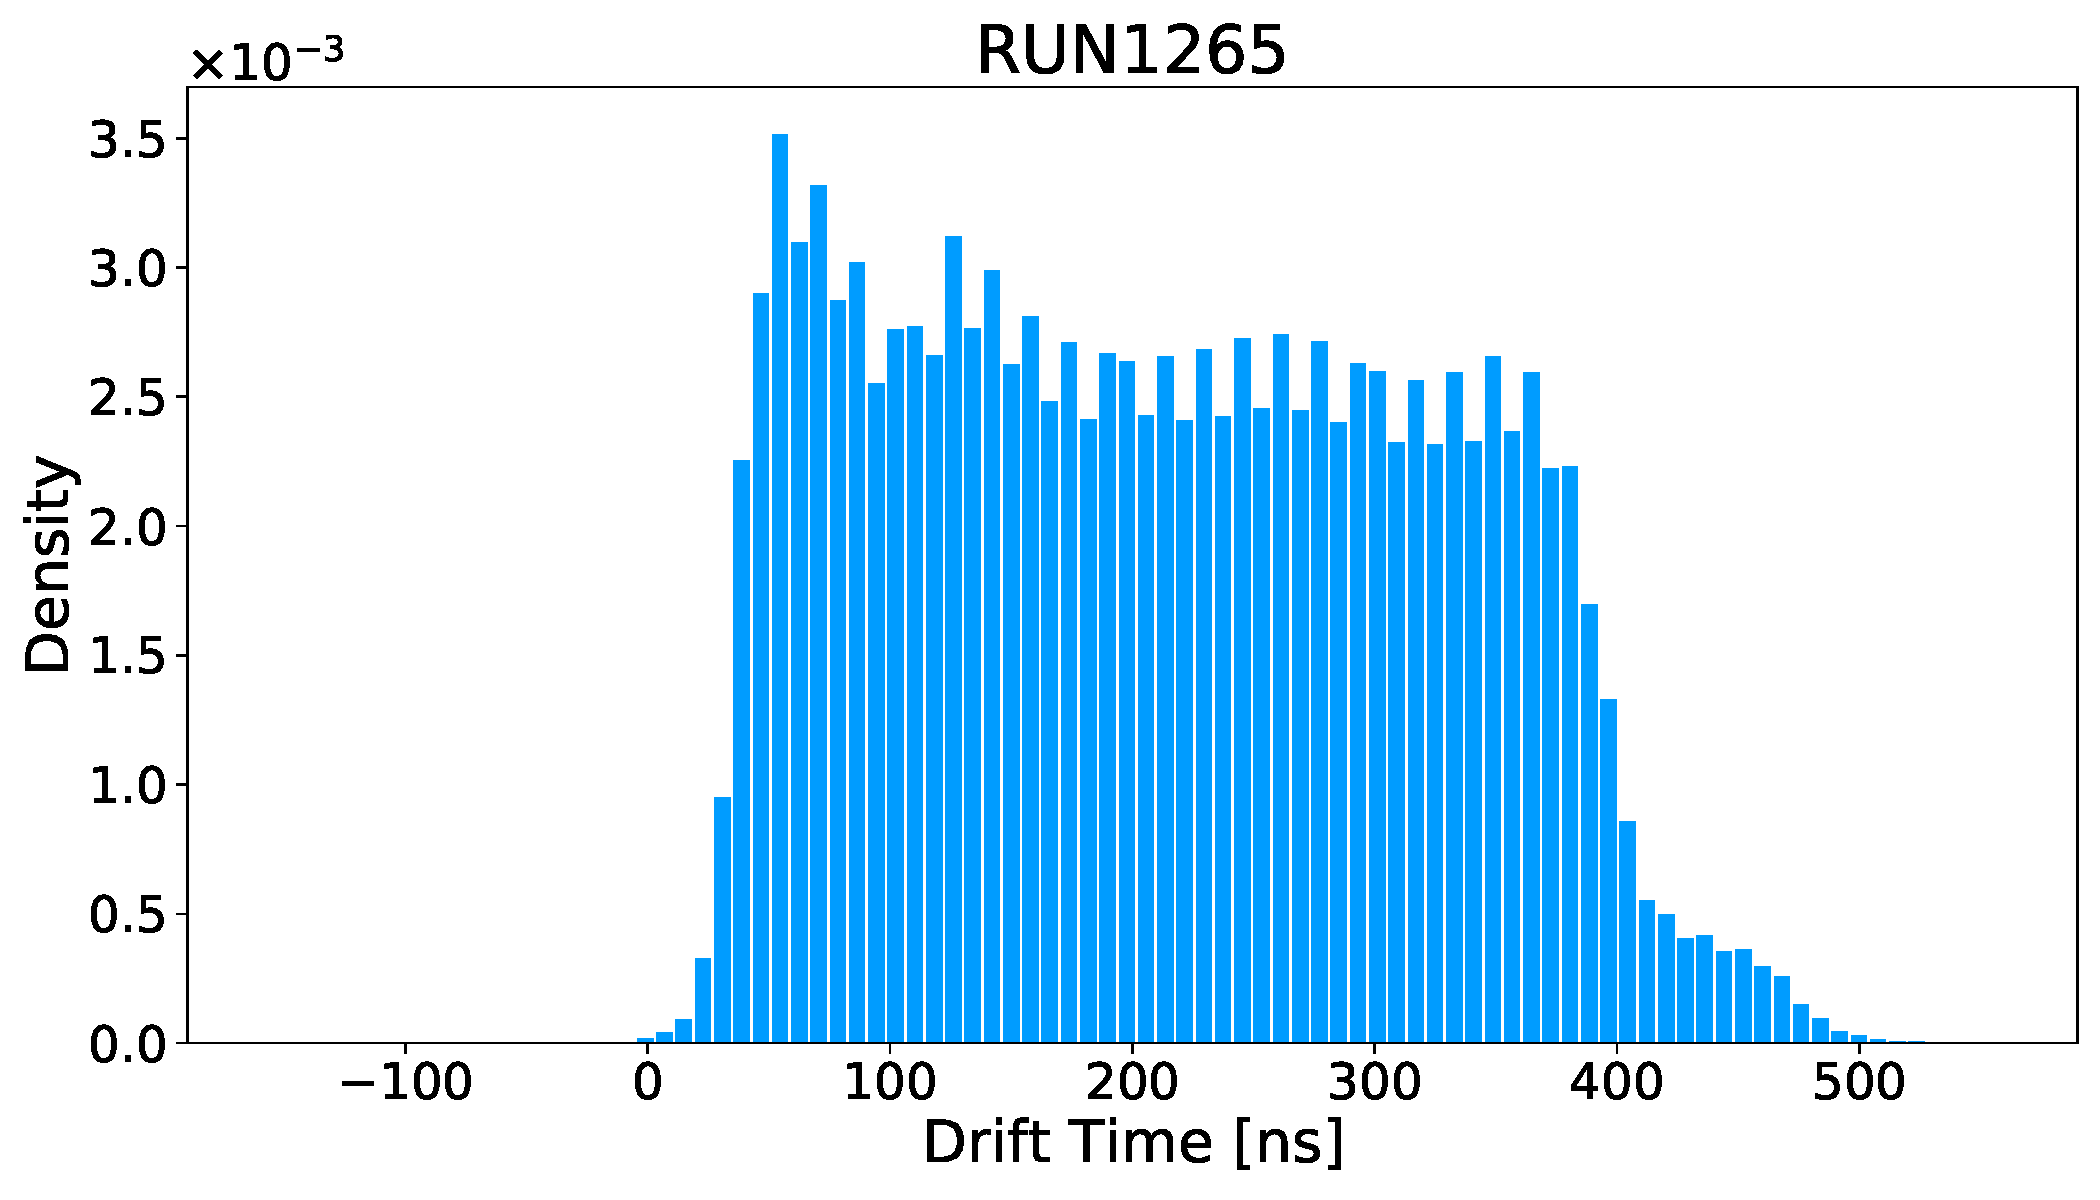
\includegraphics[width=1.0\textwidth]{./Images/1265_blue.pdf}
					\end{figure}

			\end{column}


			% RIGHT COLUMN
			\begin{column}{0.5\textwidth}

					\begin{figure}
						\centering 
						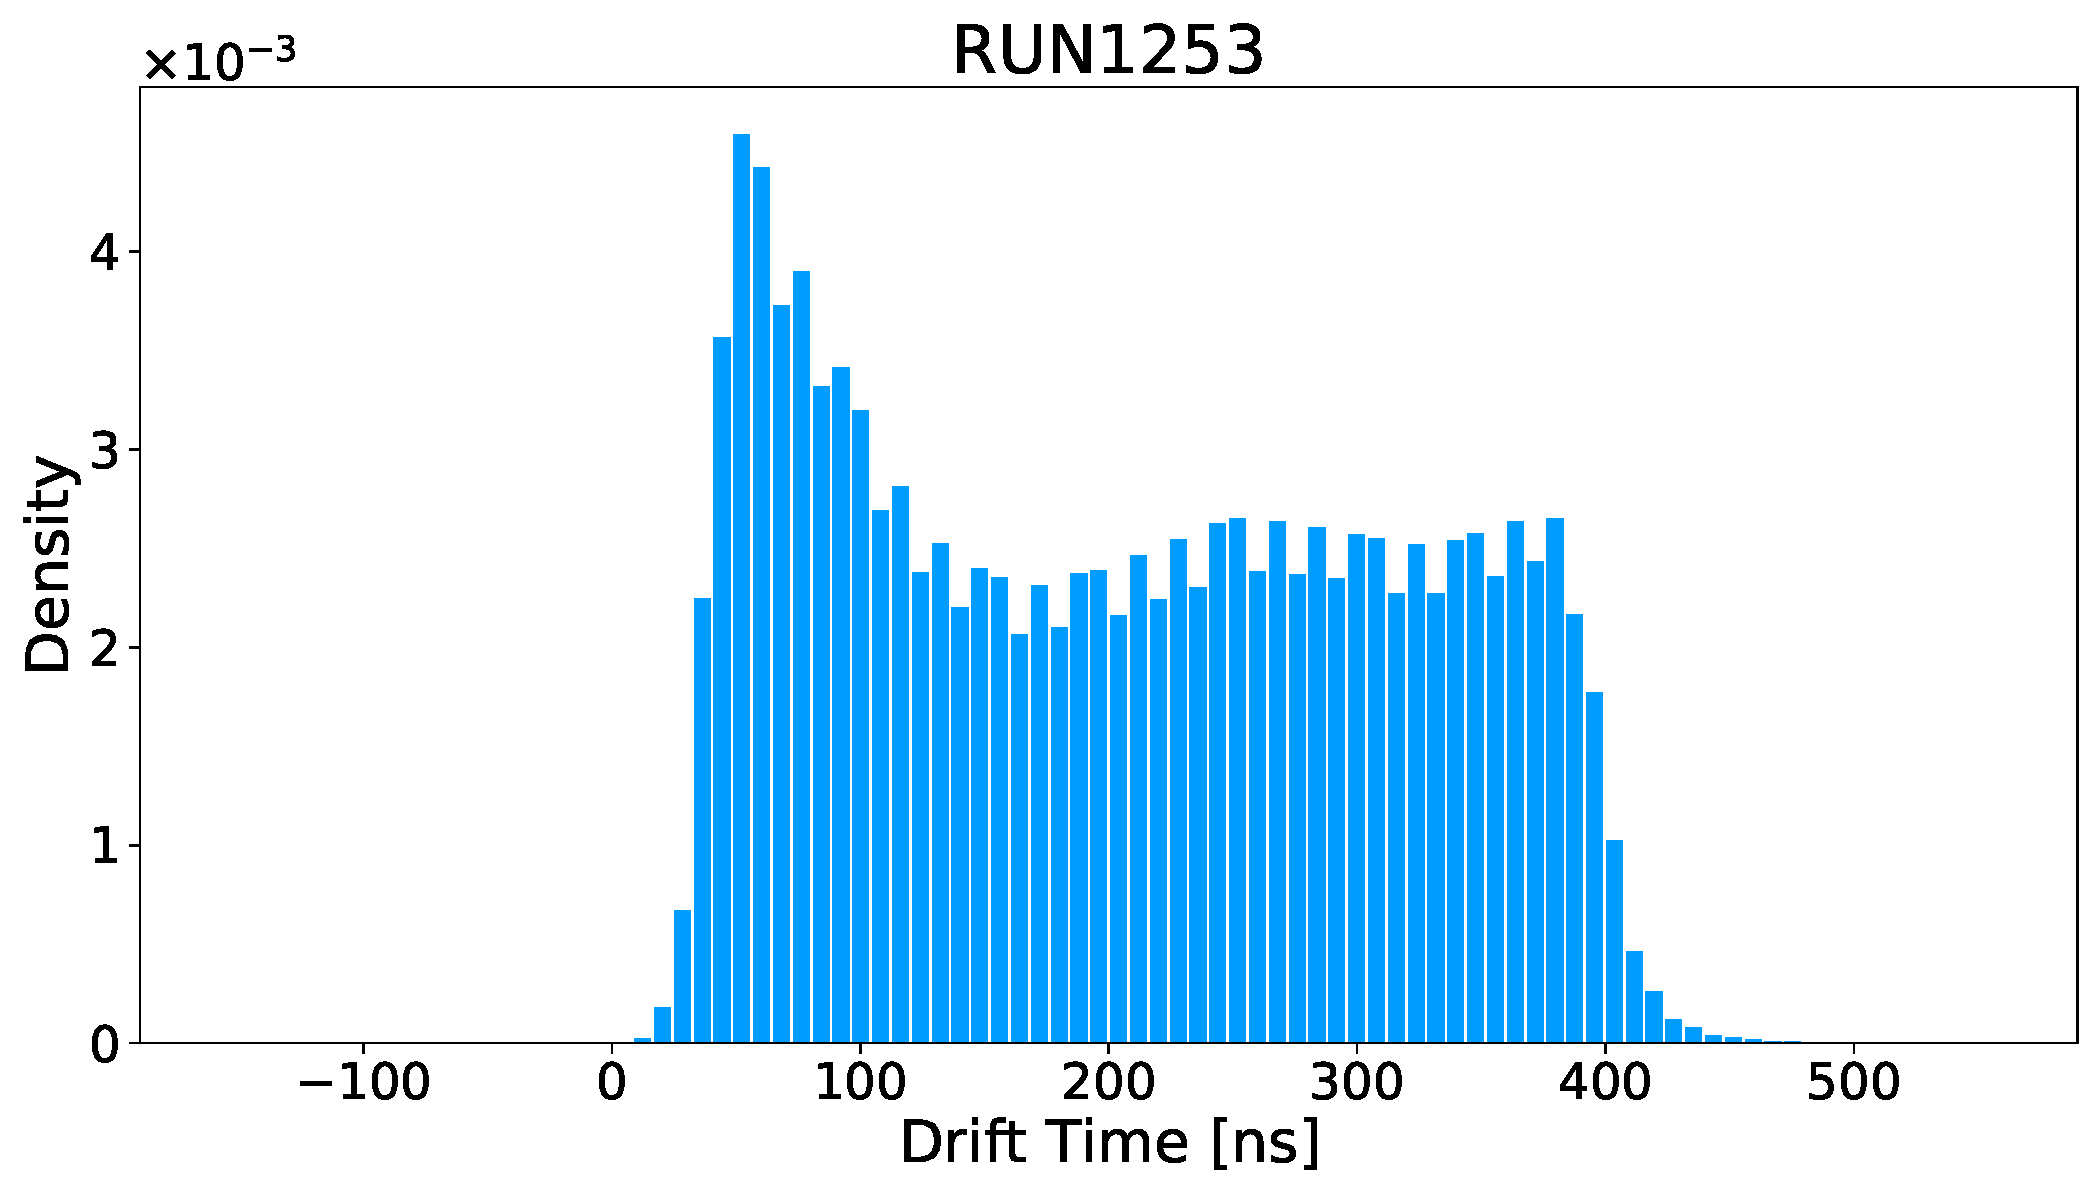
\includegraphics[width=1.0\textwidth]{./Images/1253_blue.pdf}
						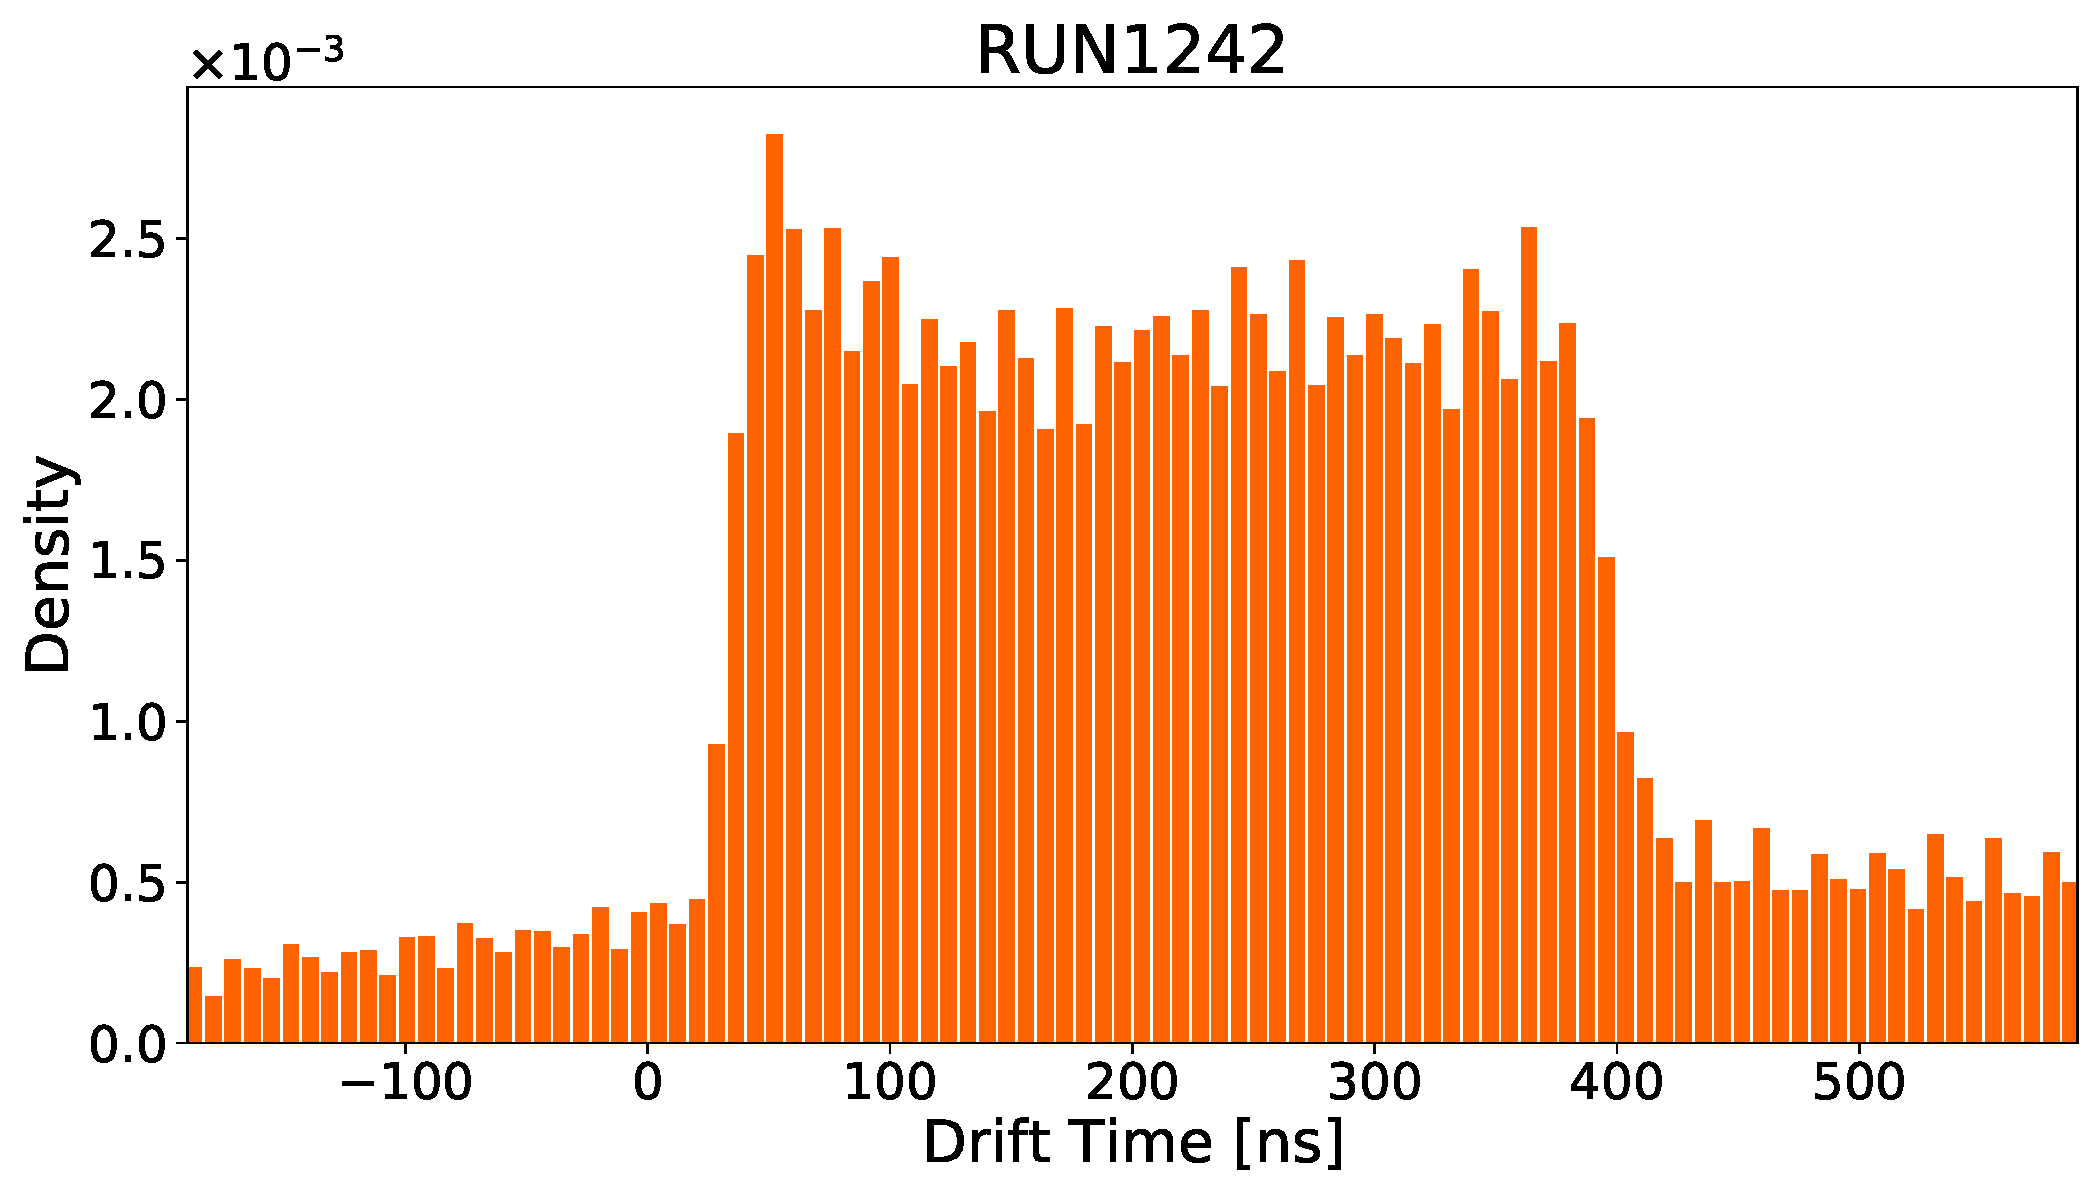
\includegraphics[width=1.0\textwidth]	{./Images/1242_orange.pdf}
					\end{figure}

			\end{column}
		\end{columns}
		}<4>

		\vfill

	\end{frame}

	\begin{frame}
		\frametitle{Testing the algorithm performance}
		\framesubtitle{Discrepancy assessment}

		\vspace{-1.5em}

		\only{
			\begin{figure}
				\centering 
				\includegraphics<1>[width=1\textwidth]{../PLOTS/DRIFT_TIME/thesis/t_obs_1.pdf}
			\end{figure}	 
		}<1>
		\only{
			\begin{figure}
				\centering 
				\includegraphics<2>[width=1\textwidth]{../PLOTS/DRIFT_TIME/thesis/t_obs_2.pdf}
			\end{figure}	 
		}<2>
		\only{
			\begin{figure}
				\centering 
				\includegraphics<3>[width=1\textwidth]{../PLOTS/DRIFT_TIME/thesis/t_obs_3.pdf}
			\end{figure}	 
		}<3>
	
	\end{frame}

	\begin{frame}
		\frametitle{Testing the algorithm performance}
		\framesubtitle{Neural network's data reconstruction}

		\vspace{-1.5em}

		\Wider{
			\begin{figure}
				\centering 
				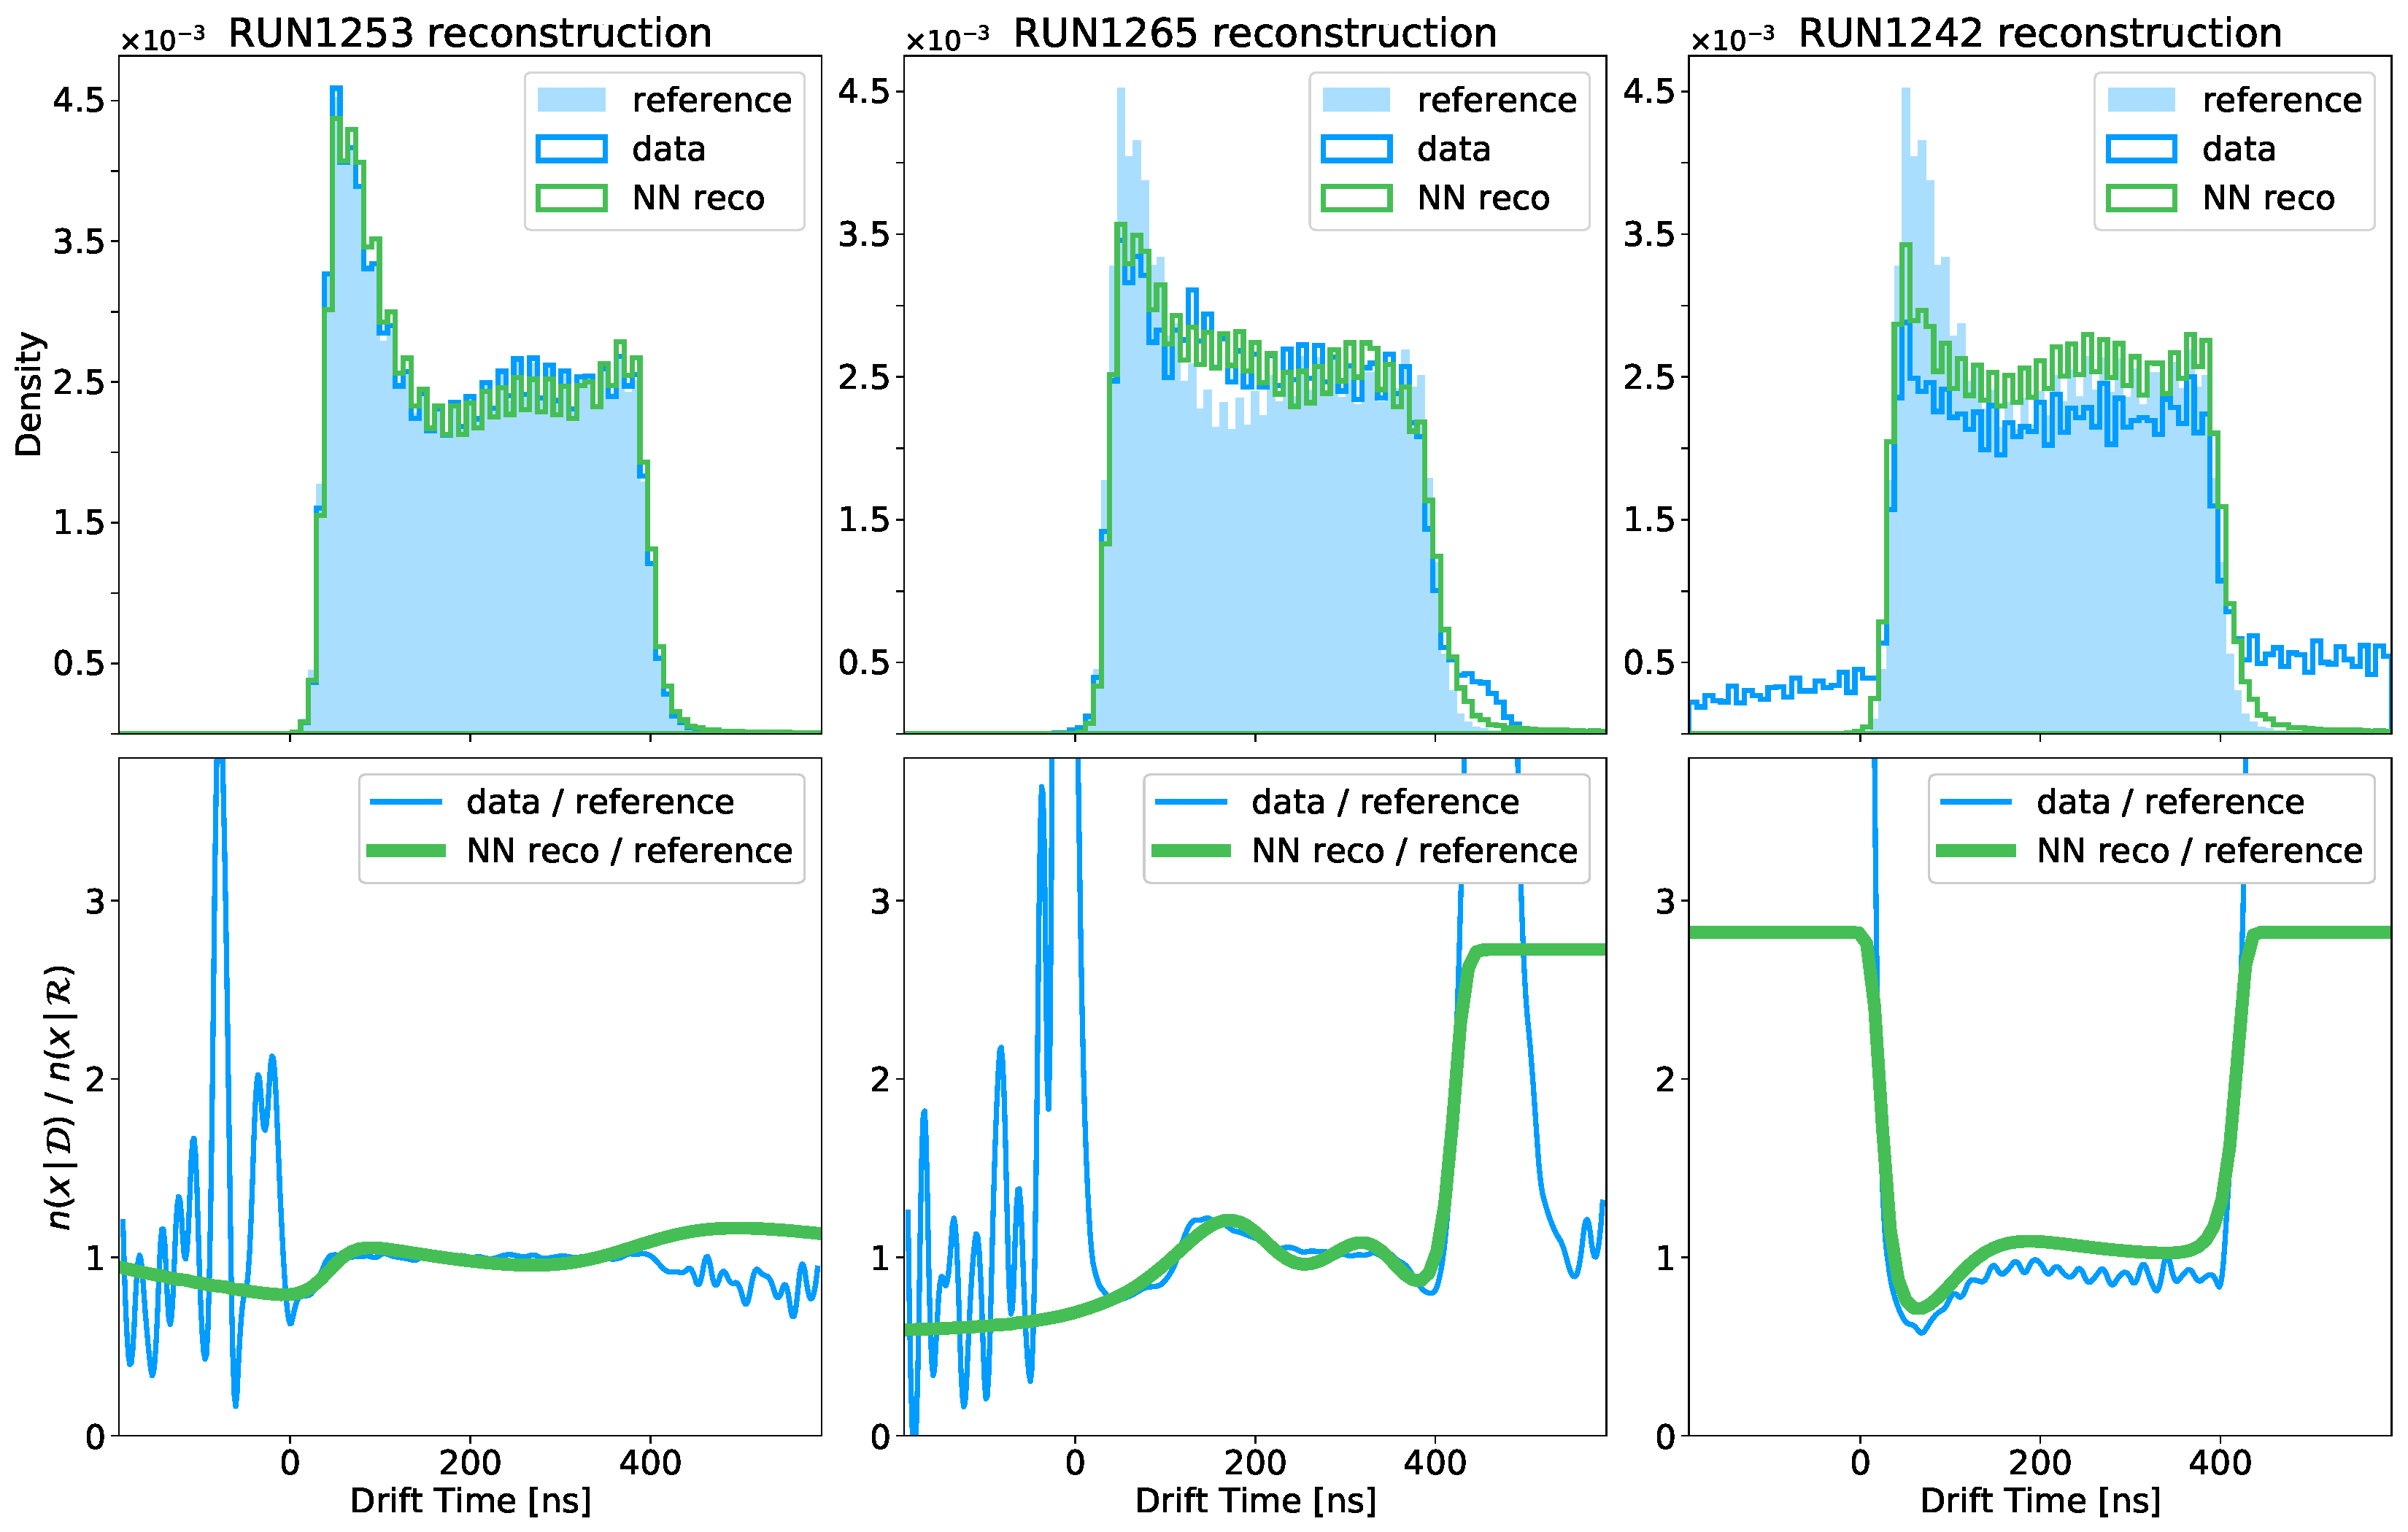
\includegraphics[width=0.9\textwidth]{../FALKON/plots/nn_reco.pdf}
			\end{figure}
		}

	\end{frame}


	% -------- SUMMARY
	\section{Summary}
	\begin{frame}
		\frametitle{Summary of the Results}
		\framesubtitle{Improving the procedure automation}

		% \onslide<1->
		The current implementation of the algorithm
		\begin{itemize}
			\item correctly detects discrepancies between $\mathbfcal{R}$ and $\mathbfcal{D}$
			\item returns larger $t_{\text{obs}}$ when the anomalies are more evident
		\end{itemize}

		\vfill

		% \onslide<2>
		However
		\begin{itemize}
			\item the most critical anomalies are not always the most obvious
			\item the time box shape may vary for other reasons \\ (e.g. due to correlations with other observables)
		\end{itemize}

	\end{frame}


	% ------------- DRIFT TIME - ANGLE CORRELATION
	\begin{frame}
		\frametitle{Example of Correlated Observables}
		\framesubtitle{Correlation between time box shape and muon crossing angle}
		
		\Wider{
			\begin{figure}
				\centering 
				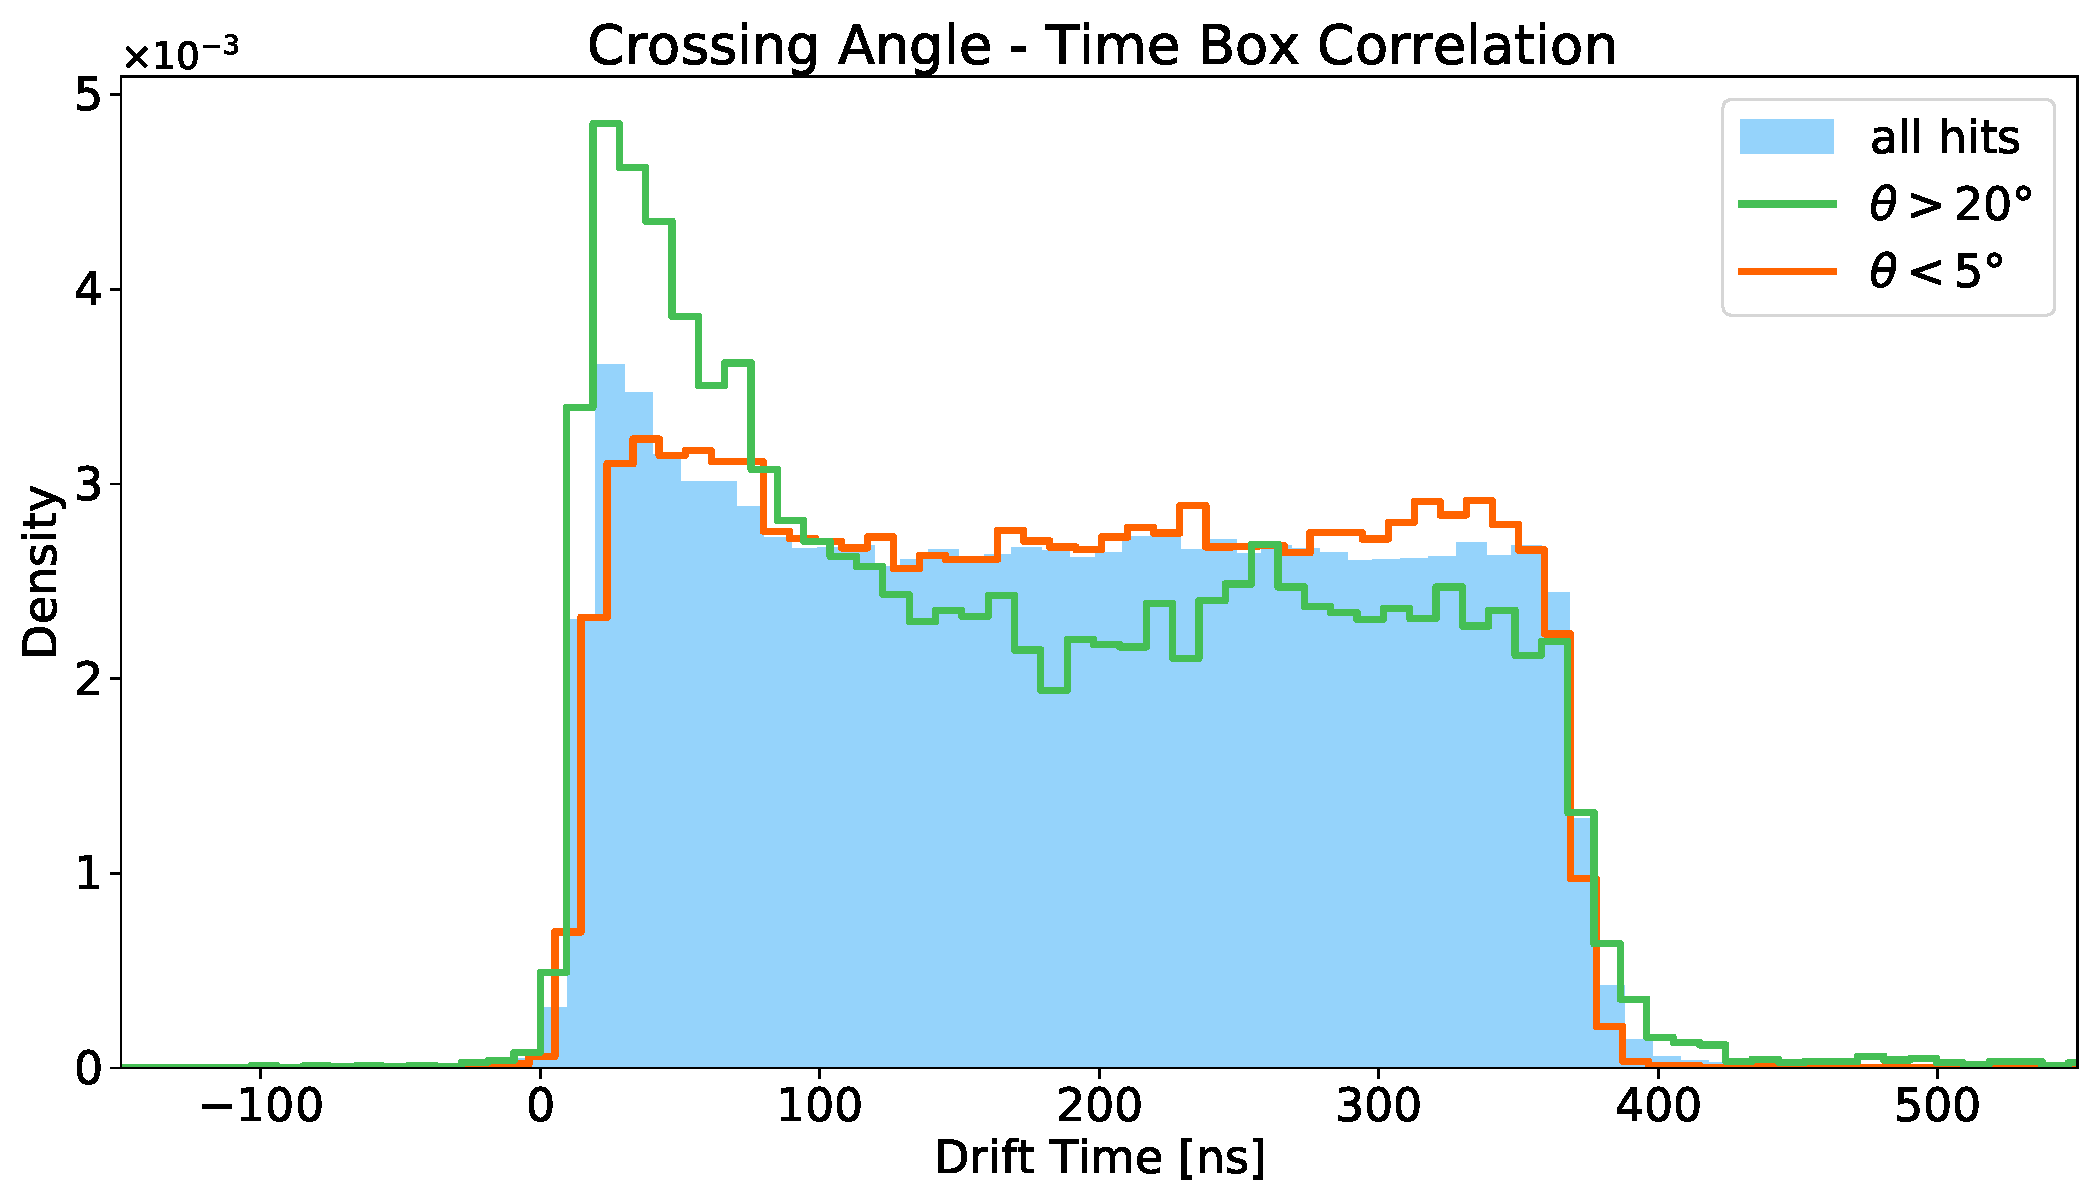
\includegraphics[width=0.9\textwidth]{../FALKON/plots/crossing_angle_corr.pdf}
			\end{figure}
		}
	\end{frame}


	% -------- FUTURE DEV
	\section{Future Developments}
	\begin{frame}
		\frametitle{Future Outlook}
		\framesubtitle{Procedure improvements}

		\begin{enumerate}
			\item Gathering correlated observables to improve flexibility
				\begin{itemize}
					\item multi-dimensional input datasets
				\end{itemize}
				\vfill
			\item Mapping different data anomalies to the corresponding detector failures
				\begin{itemize}
					\item systematic study of discrepant data collected with well-known detector setups
				\end{itemize}
				\vfill
			\item Building an \alert{\textit{online}} DQM framework for full automation
				\begin{itemize}
					\item the current implementation of the algorithm is too slow 
					\item FalkonML$^{1}$ can be exploited to emulate our algorithm 
					\item training time lowers from $\sim 47\,\text{min}$ to $\sim$\alert{$2\,\text{sec}$}
				\end{itemize}
		\end{enumerate}


		% \vfill

		\scriptsize
		$^{1}$ GitHub repository: \url{https://github.com/FalkonML/falkon}

		
	\end{frame}






	% ------------- BACKUP SLIDES
	\appendix

	% ------------- FINAL SLIDE
	\section{Final slide}
	\begin{frame}
		\centering
		\Huge
		\bfseries
		{\color{white}
		Thank you for \\ your attention!}
	\end{frame}



	\section{Backup}


	% ------------- DRIFT TUBES
	\begin{frame}
		\frametitle{Drift Tubes}
		\framesubtitle{Specifics of the detector elementary cells}
		\begin{itemize}
			\item DTs' transverse cross section  is \alert{$L\times h = 42 \times 13 \,\si{\mm}^2$}
			\item Filled with an \alert{$\text{Ar-CO}_2\,(85/15\,\%)$} gas mixture at $\sim 1\,\text{atm}$
			\item Precise electrode configuration ensures \alert{$\vec{E}\simeq \text{uniform}$} inside DTs
			\item Almost \alert{constant drift velocity} $v_{\text{drift}}\approx 54\,\si{\um/\ns}$
		\end{itemize}
		% --- DRIFT TUBE FIGURE
		\begin{center}
				\tikzset{circ/.style={circle, inner sep=0pt, minimum size=0.8cm, fill=blue!50, draw=black, text=white, align=center}}

\resizebox{!}{0.35\framewidth}{%
\begin{tikzpicture}

    % CELL
    \node(cell){\tikz {\filldraw[very thick,fill=black!5] (0, 0) rectangle ++(7,4);}};

    % WIRE
    \node(wire)[circ, minimum size=0.3cm, fill=black] at ($(cell.center)$) {};
    \node(wire-label)[above left = 0.3cm and 0cm of wire, align=center] 
    {\bfseries\large  anodic wire \\ $V_{\text{wire}}=+3.6\,\si{\kilo\volt}$};
    \draw[bend right,->, very thick, shorten <=2pt, shorten >=2pt] 
    (wire-label) to node [auto] {} (wire);

    % LEFT-WALL
    \node(left-wall)[left=-0.2cm of cell]
    {\tikz {\filldraw[very thick,fill=red, color=red] (0,0) rectangle (0.2,4);}};
    \node(left-wall-label)[above left = 0.3cm and 0cm of left-wall, align=center, color=red] 
    {\bfseries\large  cathodic side-walls \\ $V_{\text{cathod}}=-1.8\,\si{\kilo\volt}$};
    \draw[bend right,->, very thick, shorten <=2pt, shorten >=2pt, color=red] 
    (left-wall-label) to node [auto] {} (left-wall);

    % RIGHT-WALL
    \node(right-wall)[right=-0.2cm of cell]
    {\tikz {\filldraw[very thick,fill=red, color=red] (0,0) rectangle (0.2,4);}};

    % TOP-WALL
    \node(top-wall)[above=-0.2cm of cell]
    {
        \tikz {
            \filldraw[very thick,fill=blue, color=blue] (0,0) rectangle ++(1.2,0.2);
        }
        \tikz {
            \filldraw[very thick,fill=blue, color=blue] (0,0) rectangle ++(1.2,0.2);
        }
        \tikz {
            \filldraw[very thick,fill=blue, color=blue] (0,0) rectangle ++(1.2,0.2);
        }
        \tikz {
            \filldraw[very thick,fill=blue, color=blue] (0,0) rectangle ++(1.2,0.2);
        }
    };
    \node(top-wall-label)[above right = 0.3cm and 0.5cm of top-wall, align=center, color=blue] 
    {\bfseries\large cathodic strips \\ $V_{\text{strip}}=-1.2\,\si{\kilo\volt}$};
    \draw[bend right,->, very thick, shorten <=2pt, shorten >=2pt, color=blue] 
    (top-wall-label) to node [auto] {} (top-wall);

    % BOTTOM-WALL
    \node(bottom-wall)[below=-0.2cm of cell]
    {
        \tikz {
            \filldraw[very thick,fill=blue, color=blue] (0,0) rectangle ++(1.2,0.2);
        }
        \tikz {
            \filldraw[very thick,fill=blue, color=blue] (0,0) rectangle ++(1.2,0.2);
        }
        \tikz {
            \filldraw[very thick,fill=blue, color=blue] (0,0) rectangle ++(1.2,0.2);
        }
        \tikz {
            \filldraw[very thick,fill=blue, color=blue] (0,0) rectangle ++(1.2,0.2);
        }
    };
         
\end{tikzpicture}}
		\end{center}
	\end{frame}



	% ------------- CONCEPTUAL FOUNDATIONS
	\begin{frame}
		\frametitle{Hypothesis testing with NNs}
		\framesubtitle{Conceptual foundations}

		\begin{itemize}
			\setlength{\itemsep}{0.6em}
			\item Null hypothesis $H_0$: \\\vspace{0.2em} 
			$n\,(x\,|\,\mathbfcal{R})$ $\longrightarrow$ data following
			the reference model $\mathbfcal{R}$
			\item Alternative hypothesis $H_1$: \\\vspace{0.2em} 
			$n\,(x\,|\,\bm{w}) =
			n\,(x\,|\,\mathbfcal{R})\,e^{f(x;\,\bm{w})}$ $\longrightarrow$ parametrized by the NN
		\end{itemize}

		\vfill

		The most powerful statistical test is the \alert{likelihood-ratio test} (Neyman-Pearson lemma)

		\vfill

		The algorithm compares $n\,(x\,|\,\mathbfcal{R})$ with $n\,(x\,|\,\bm{\widehat{w}})$ where $\bm{\widehat{w}}$ is
		the parameters configuration that maximizes the likelihood


	\end{frame}

	% ------------- WILKS THEOREM
	\begin{frame}
		\frametitle{The Wilks' Theorem}
		\framesubtitle{Asymptotic distribution of the log-likelihood ratio statistic}

		The test statistic is given by

		\begin{align*}
			t(\mathbfcal{D}) &= 2 \, \log \left[
			\frac{
				e^{-\mathcal{N}(\bm{\widehat{w}})}
			}{
				e^{-\mathcal{N}(\mathbfcal{R})}
			}
			\prod_{x \in \mathbfcal{D}}
			\frac{
				n(x\,|\,\bm{\widehat{w}})  
			}{
				n(x\,|\,\mathbfcal{R})
			}
		\right] \\
		& = 
		-2\,\min_{\bm{w}} 
		\left[
			\frac{
				\mathcal{N}(\mathbfcal{R})
			}{
				\mathcal{N}_{\mathbfcal{R}}
			}
			\sum_{x \in \mathbfcal{R}}
			\left(
				e^{\,f(x;\,\bm{{w}})} - 1
			\right)
			- \sum_{x \in \mathbfcal{D}}  f(x;\,\bm{{w}})
		\right] 
		\end{align*}

		\vfill

		Wilks' theorem states that the $t(\mathbfcal{D})$ distribution asymptotically approaches a \alert{$\chi^2$
		distribution} under the null hypothesis $H_0$

		
	\end{frame}

	% ------ TUNING
	\begin{frame}
		\frametitle{Tuning the Neural Network}
		\framesubtitle{Testing different weight clipping values}

		\vspace{-2em}

		\Wider{

			\begin{columns}[onlytextwidth]

				% LEFT COLUMN
				\begin{column}{0.33\textwidth}

						\begin{figure}
							\centering 
							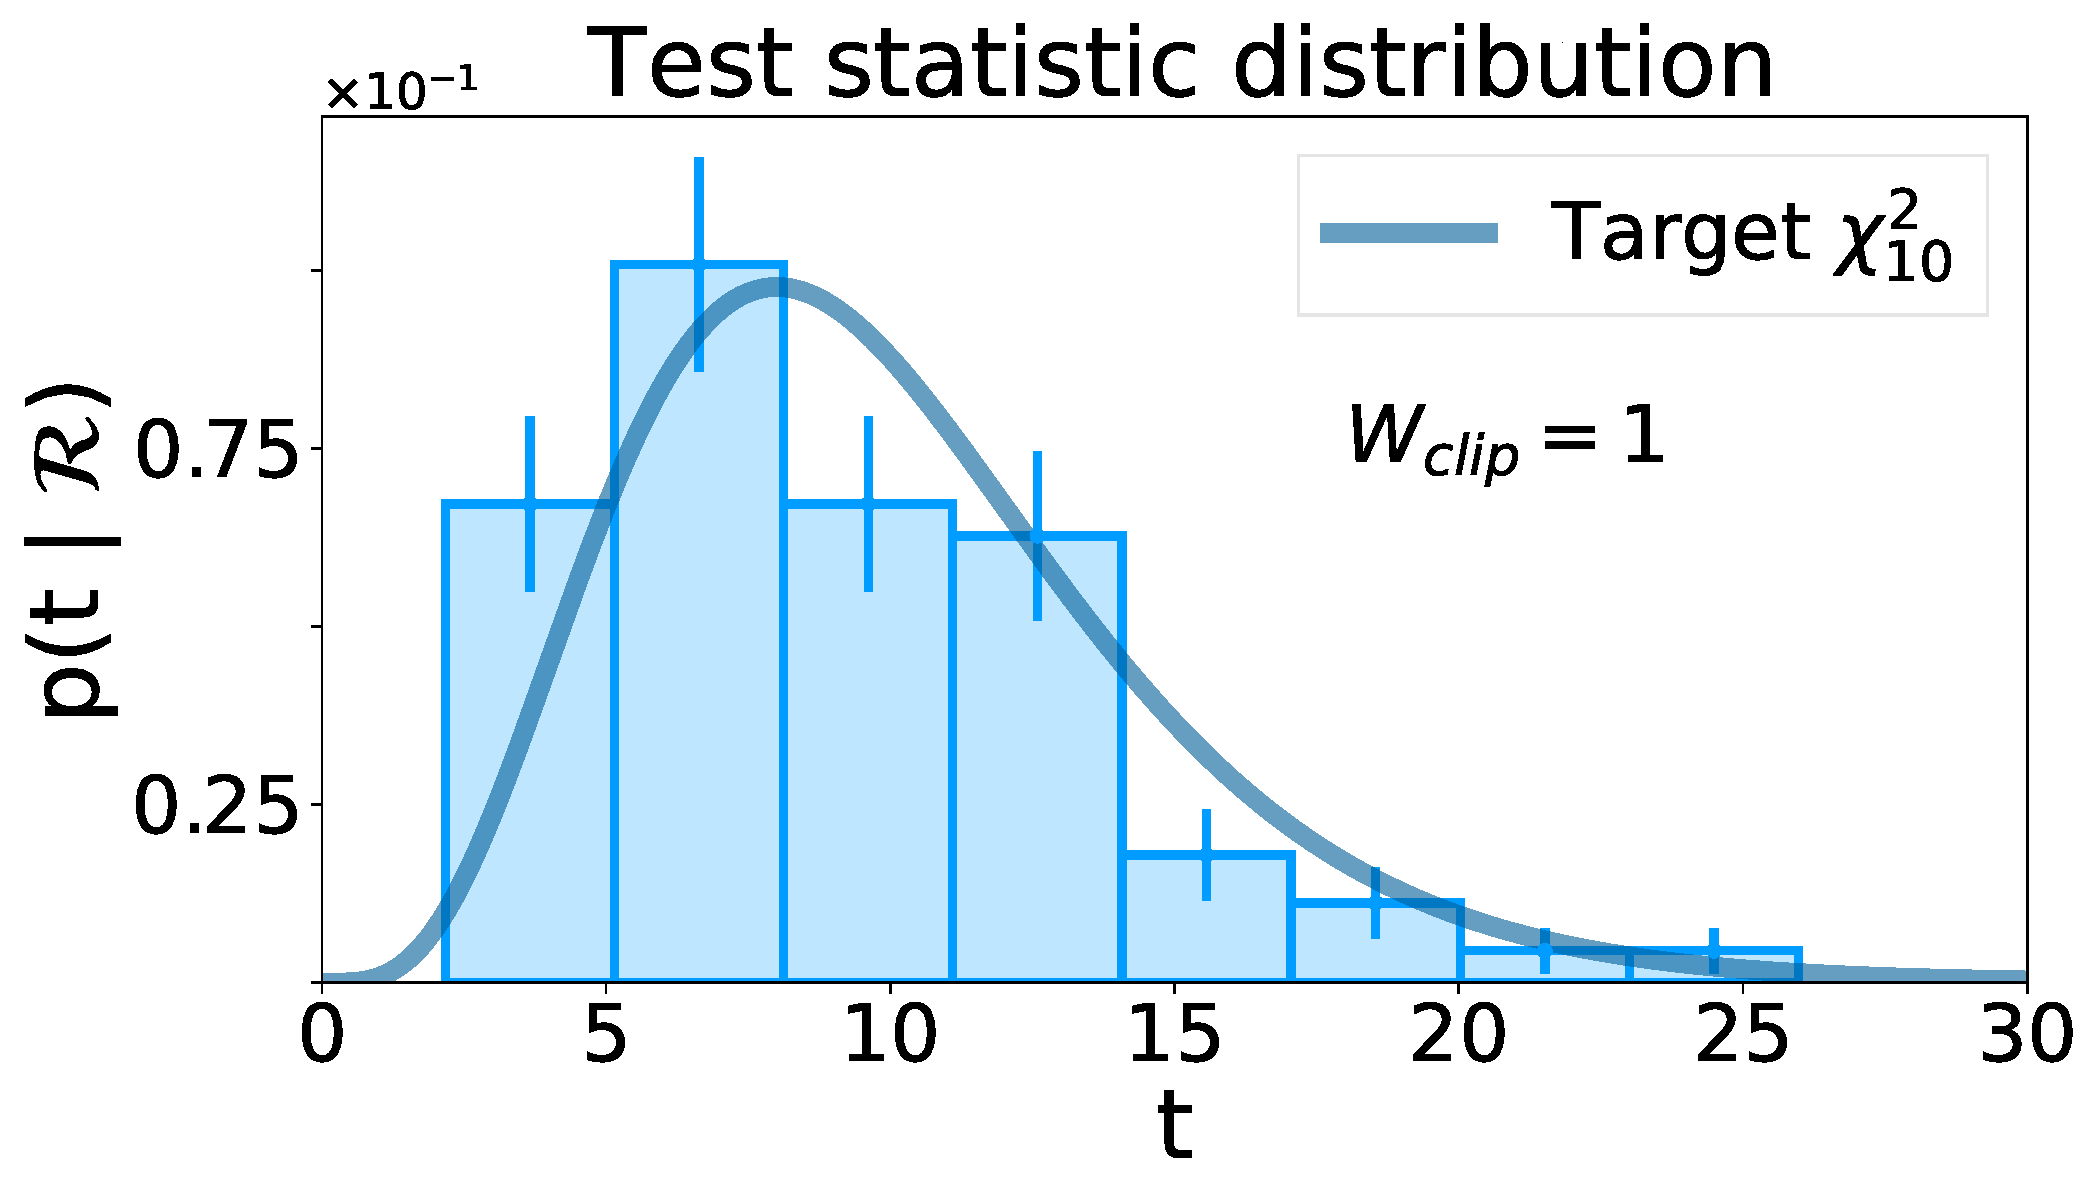
\includegraphics[width=1.0\textwidth]{../PLOTS/DRIFT_TIME/thesis/a_distribution_1_0.pdf}
							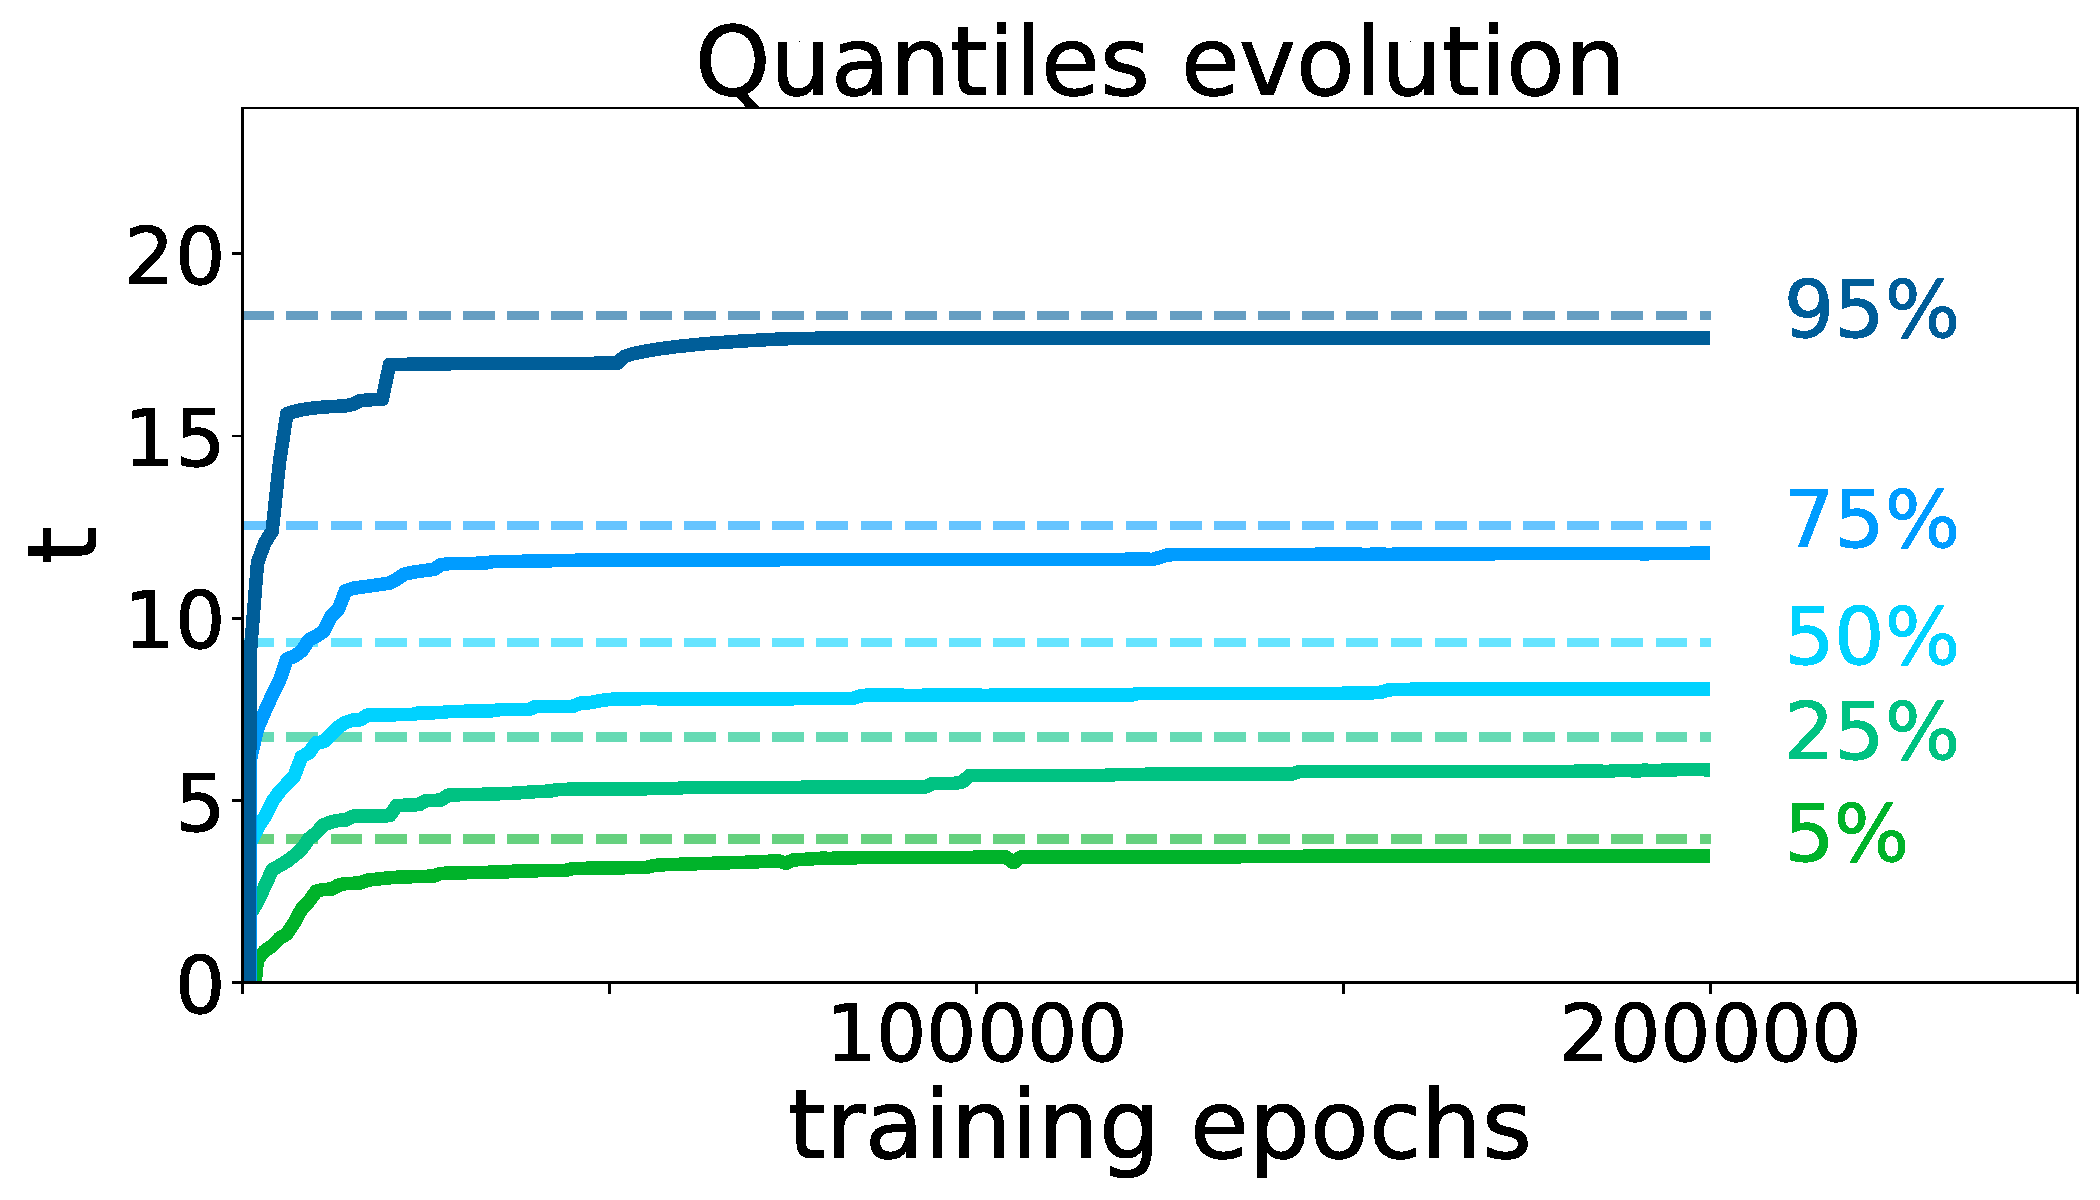
\includegraphics[width=1.0\textwidth]{../PLOTS/DRIFT_TIME/thesis/a_quantiles_1_0.pdf}
						\end{figure}

				\end{column}

				% MIDDLE COLUMN
				\begin{column}{0.33\textwidth}

						\begin{figure}
							\centering 
							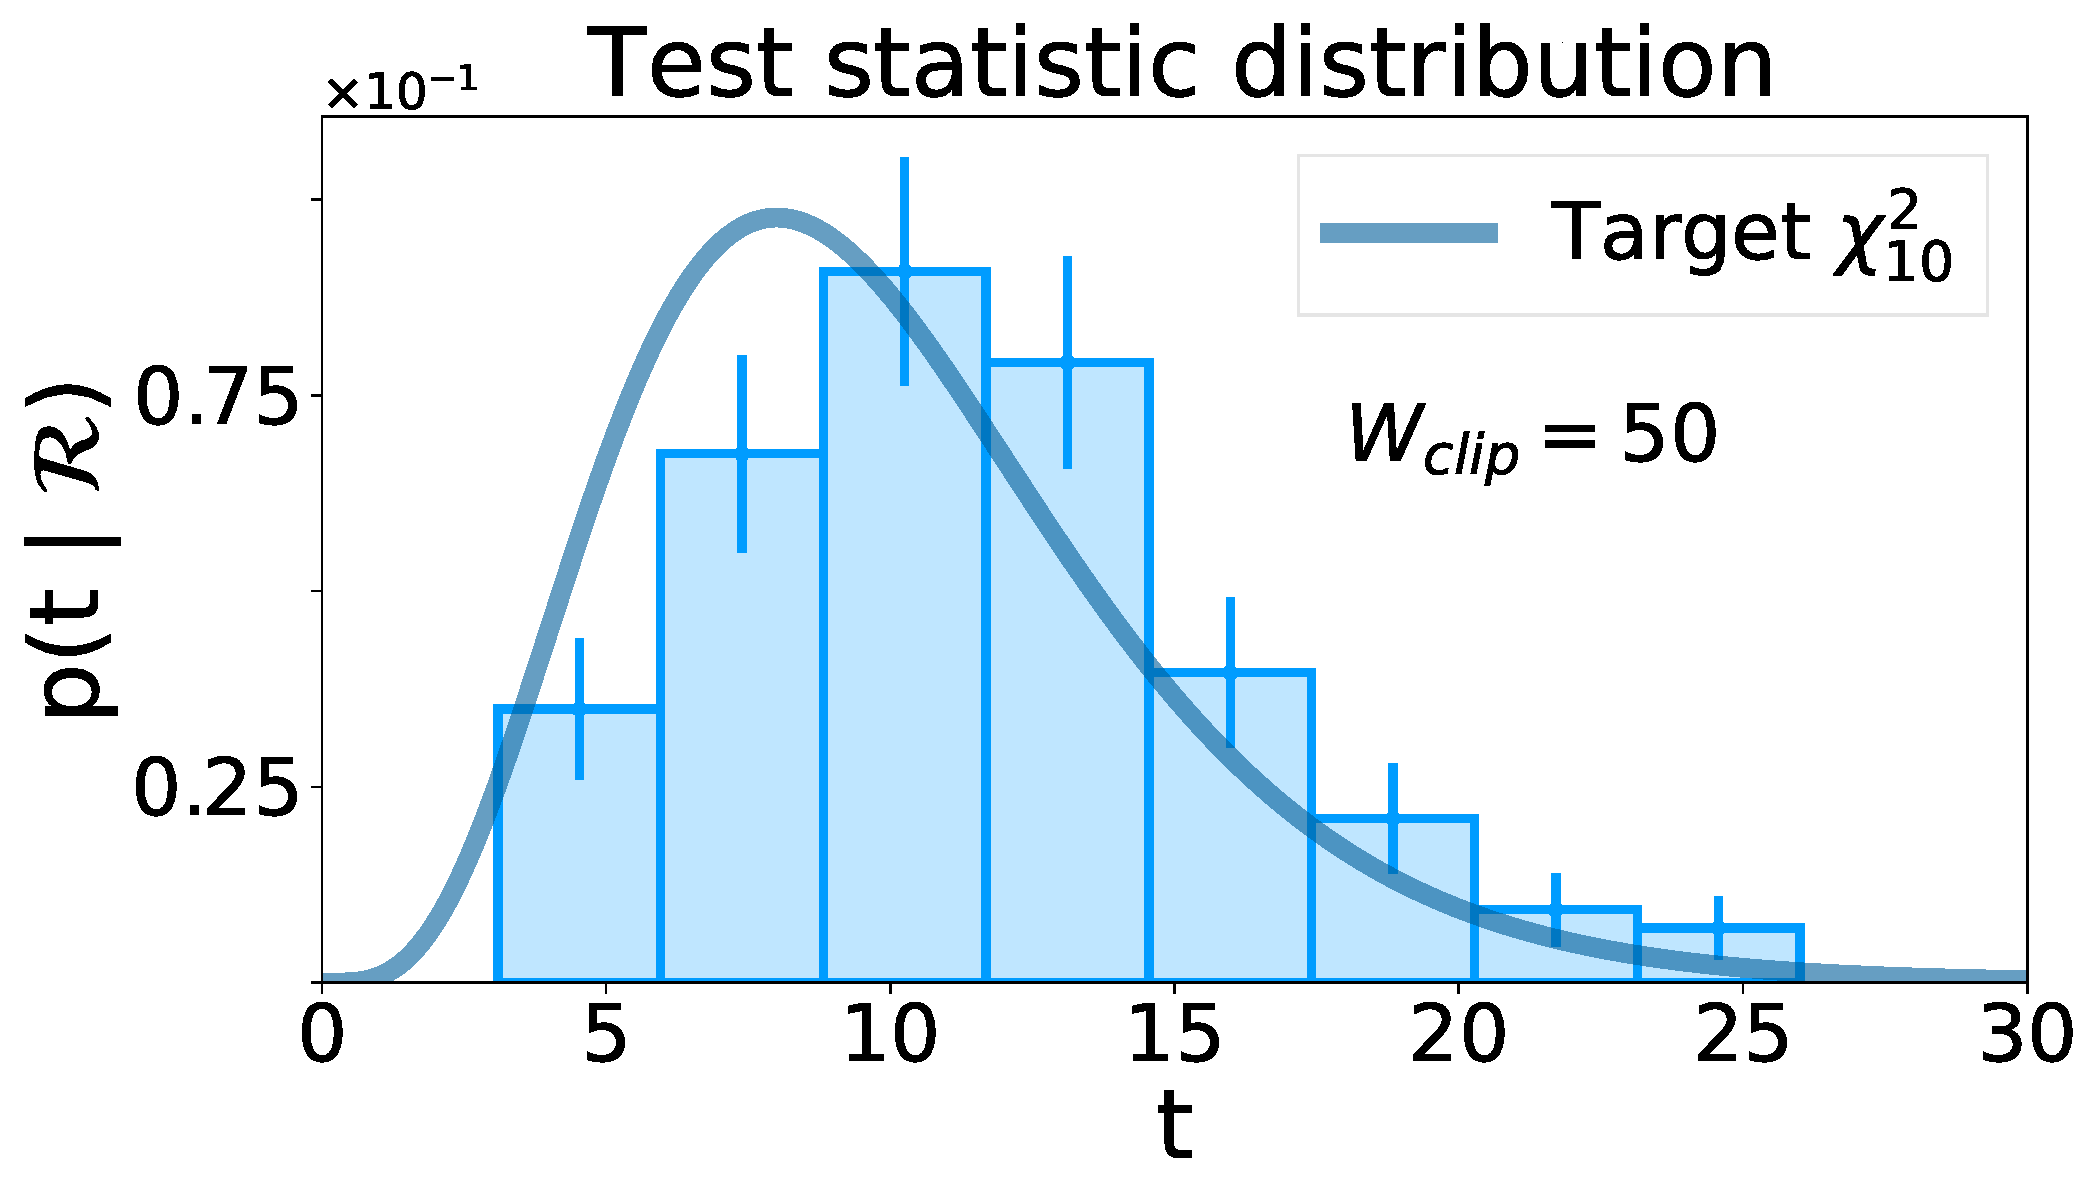
\includegraphics[width=1.0\textwidth]{../PLOTS/DRIFT_TIME/thesis/a_distribution_50_0.pdf}
							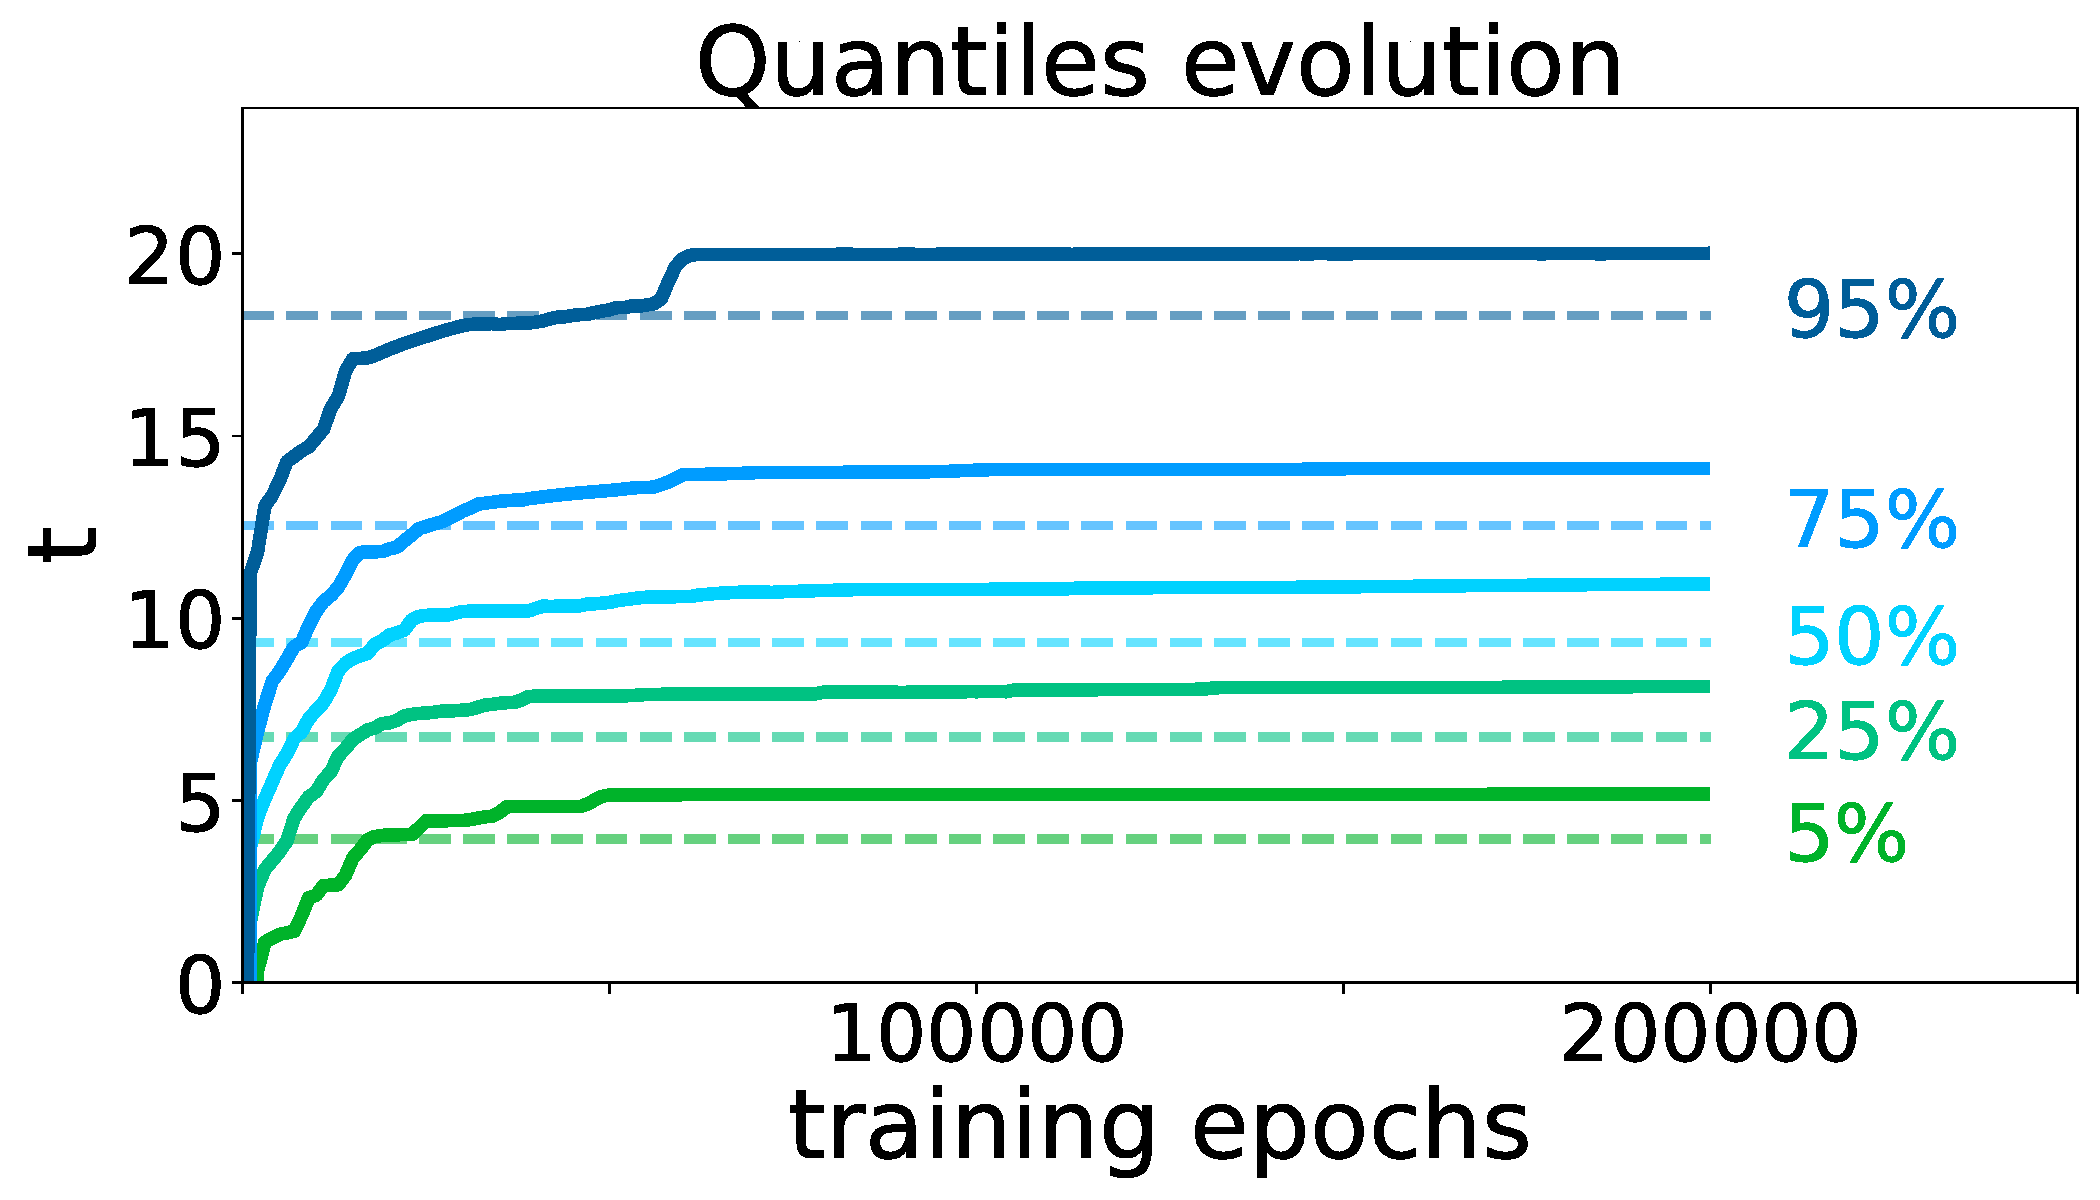
\includegraphics[width=1.0\textwidth]{../PLOTS/DRIFT_TIME/thesis/a_quantiles_50_0.pdf}
						\end{figure}

				\end{column}


				% RIGHT COLUMN
				\begin{column}{0.33\textwidth}

						\begin{figure}
							\centering 
							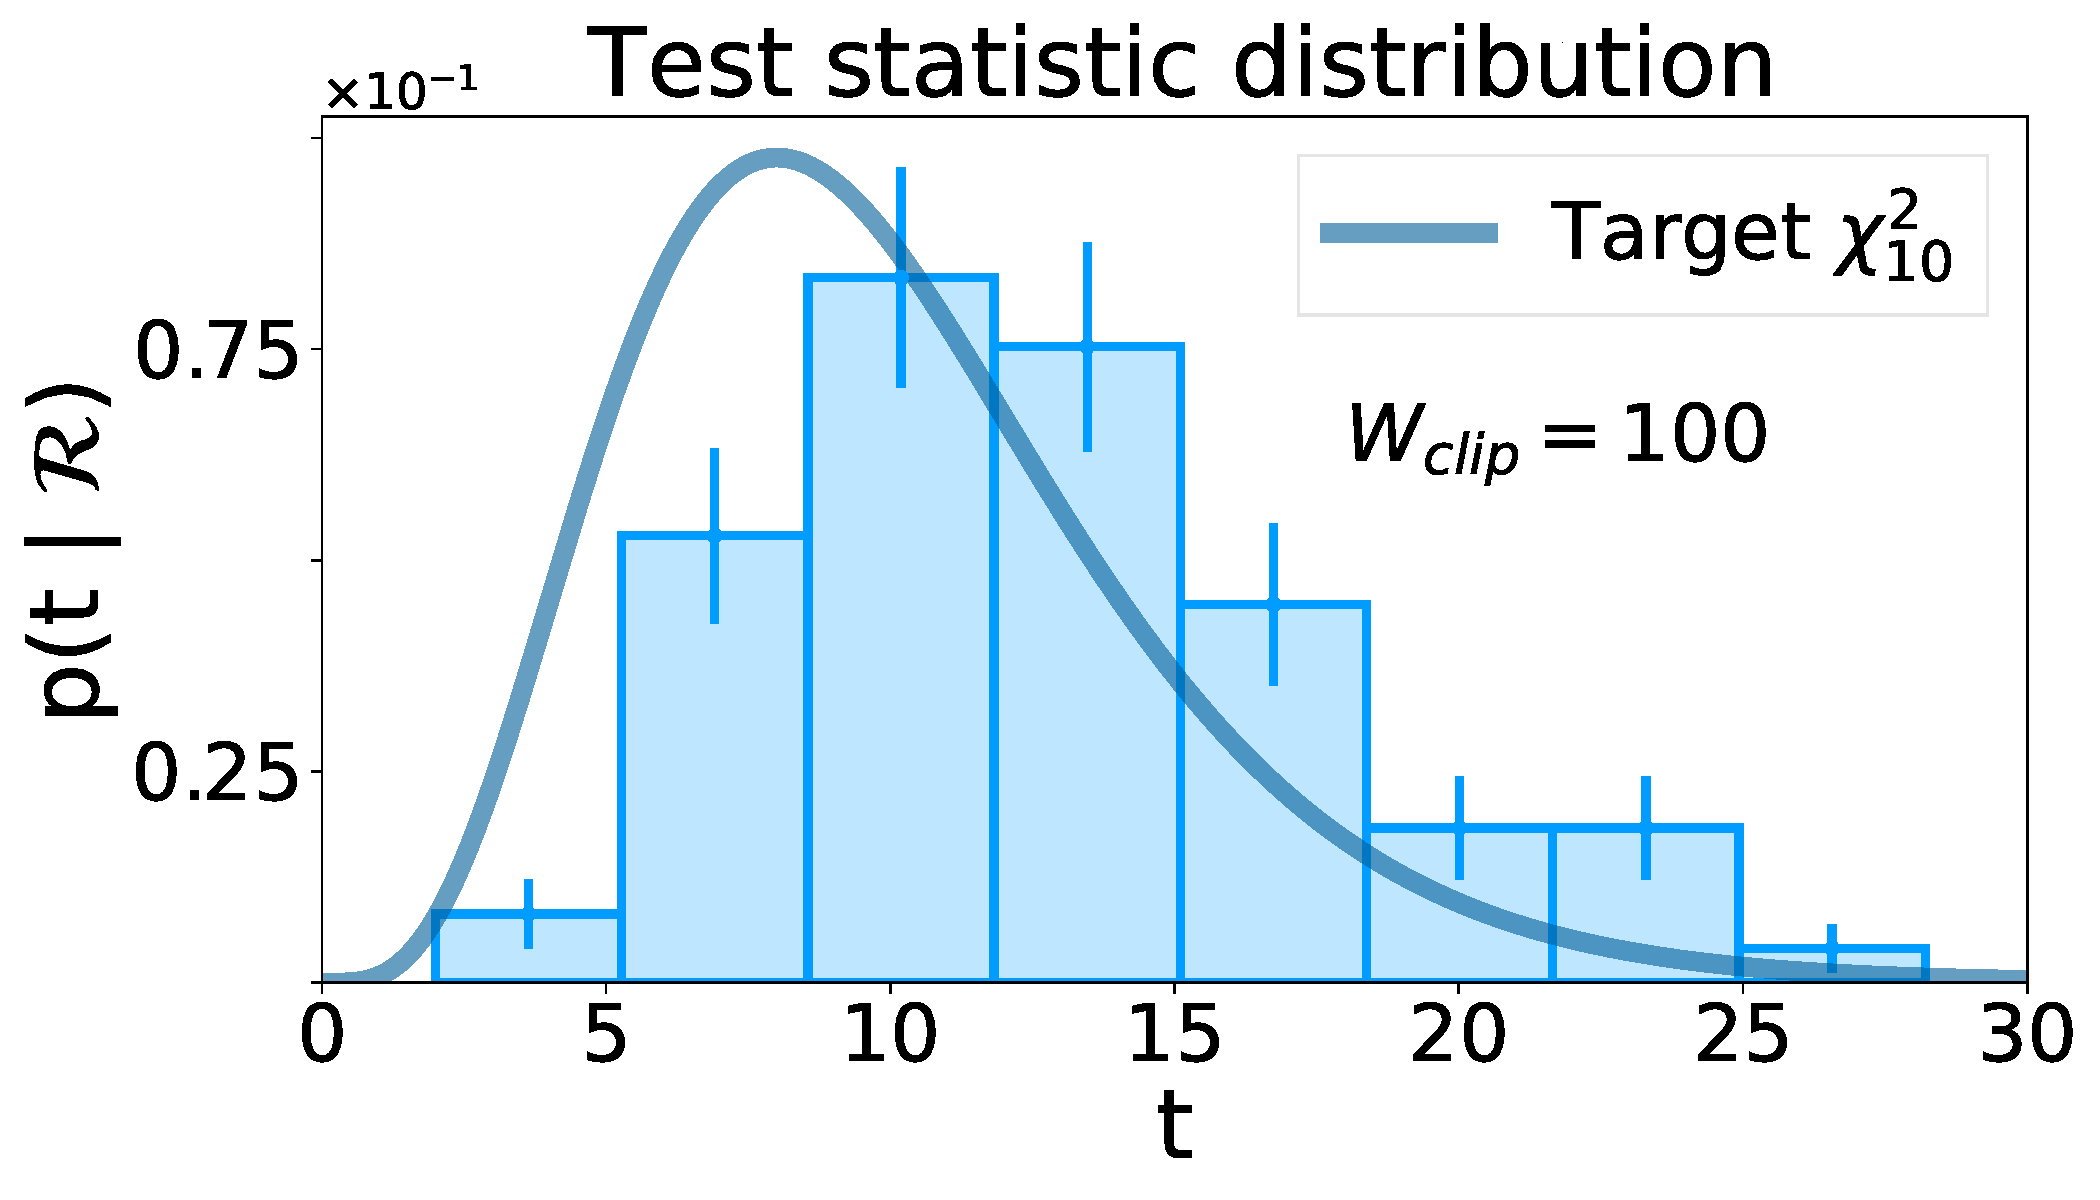
\includegraphics[width=1.0\textwidth]{../PLOTS/DRIFT_TIME/thesis/a_distribution_100_0.pdf}
							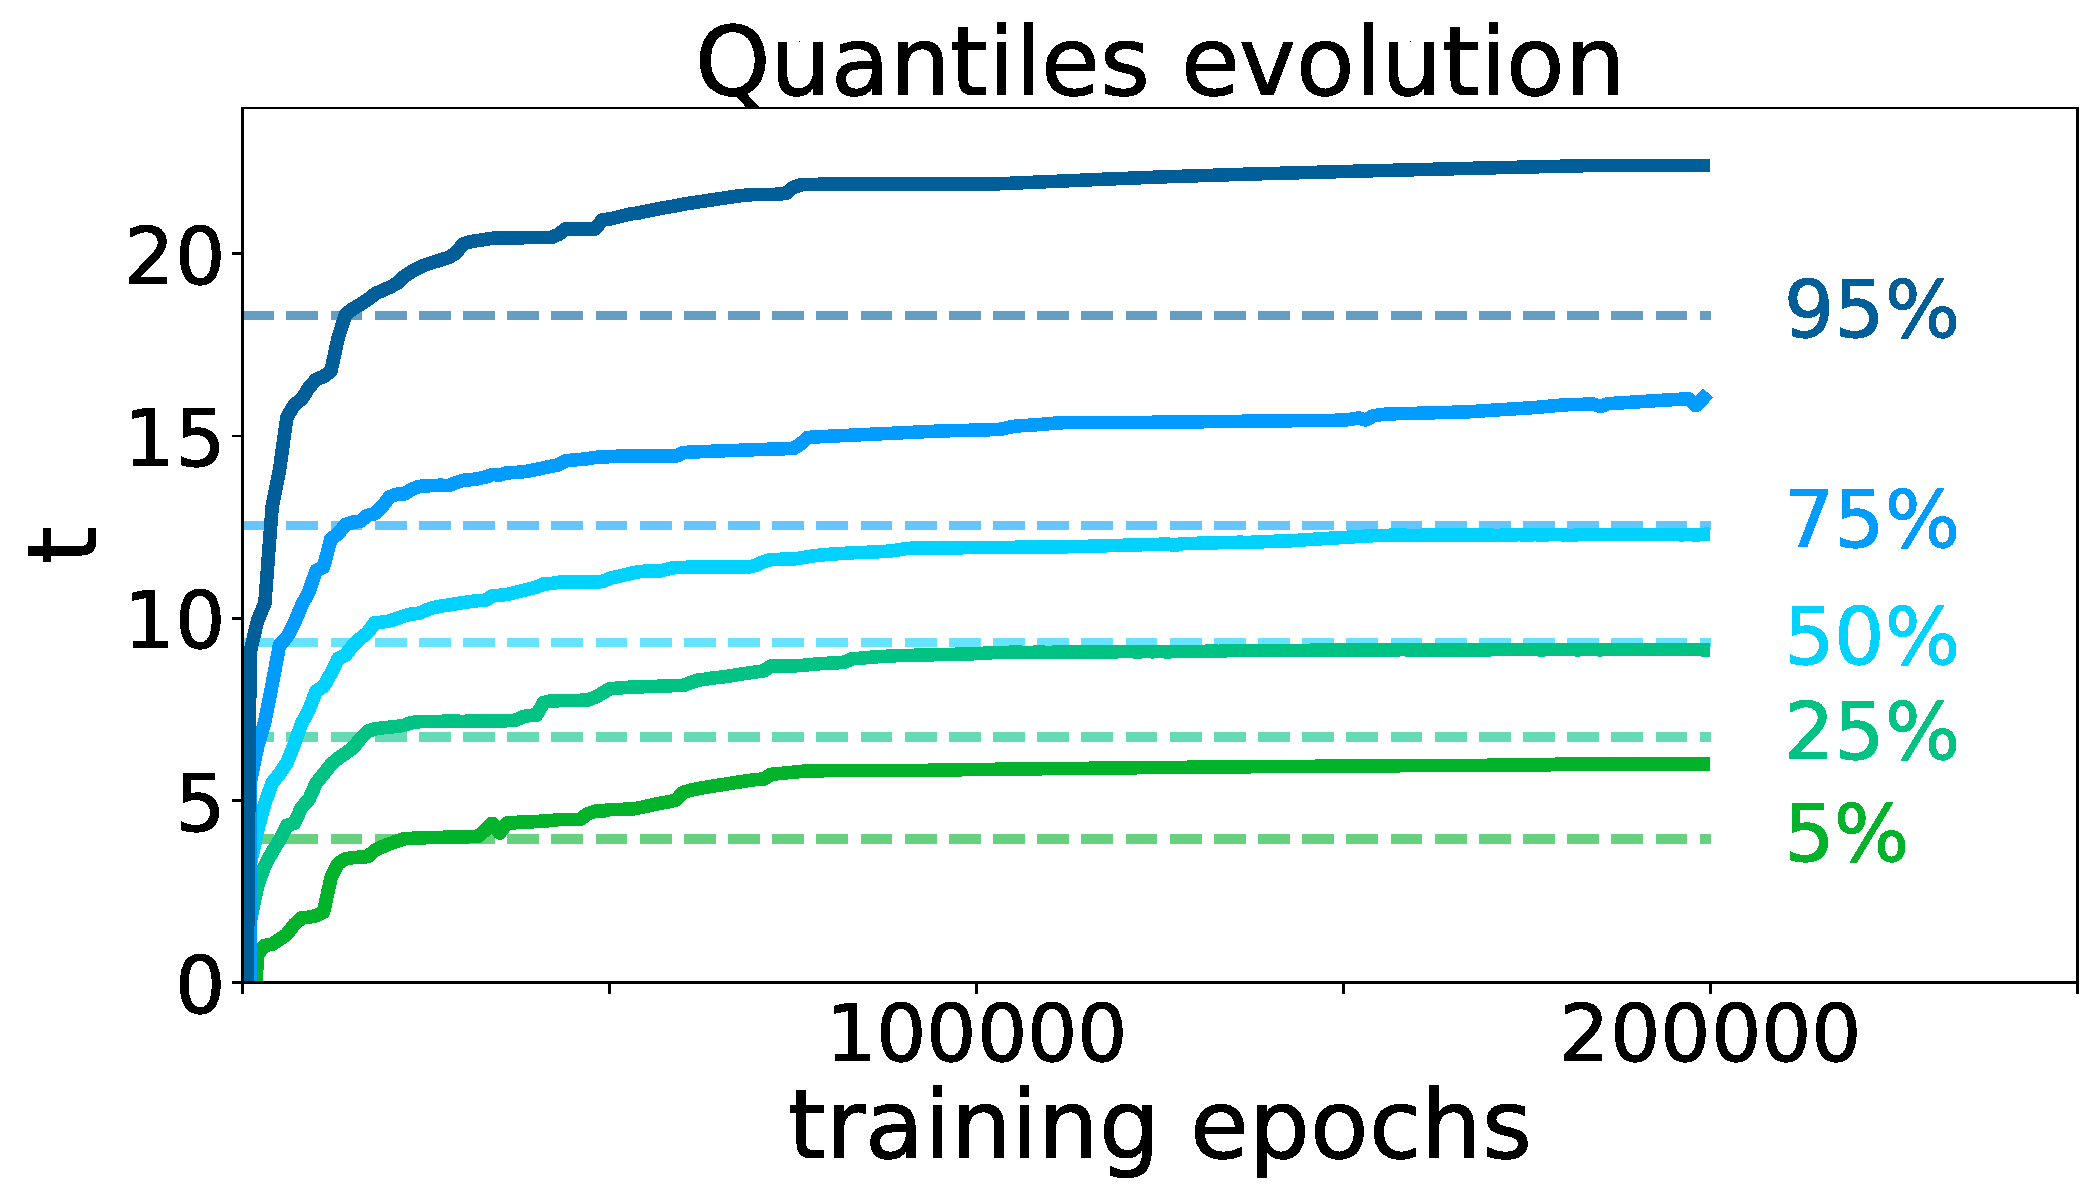
\includegraphics[width=1.0\textwidth]{../PLOTS/DRIFT_TIME/thesis/a_quantiles_100_0.pdf}
						\end{figure}

				\end{column}
			\end{columns}

		}

	\end{frame}


	% ------------- FALKONML
	\begin{frame}
		\frametitle{FalkonML}
		\framesubtitle{Data quality monitoring with kernel methods}

		Kernel methods:
		\begin{itemize}
			\item $\widehat{f}(x)=\sum_{i}\alpha_i k(x,\,x_i)$ where $k(x,\,x')=\exp(\frac{||x-x'||^2}{2\sigma^2})$
		\end{itemize}

		\vfill

		FalkonML:
		\begin{itemize}
			\setlength{\itemsep}{0.7em}
			\item implements the \alert{Nystr\"{o}m approximation} \\\vspace{0.2em}
			$\widehat{f}(x)=\sum_{i}\alpha_i k(x,\,\widetilde{x}_i)$ where $\{\widetilde{x}_i\}_{i=1}^{m} \subset
			\{x_i\}_{i=1}^{n}$
			\item uses the \alert{logistic loss function} \\\vspace{0.2em}
			$L[f] = \frac{
				\mathcal{N}(\mathbfcal{R})
			}{
				\mathcal{N}_{\mathbfcal{R}}
			}
			(1-y)
			\log(1+e^{f(x;\,\bm{{w}})})
			+ y\log(1+e^{-f(x;\,\bm{{w}})})
			$
			\item the test statistic $t(\mathbfcal{D})$ is computed using $f(x;\,\bm{\widehat{w}})$
			
		\end{itemize}

		\vfill

		

		
	\end{frame}

\end{document}
